\doublespacing
\section{Introduction}
In the last chapter, we have given some attention to a methodology that allows us to use functional data for reduced form analysis. In this chapter, we focus on the economic questions that can be asked using such a methodology. Specifically, we focus on an investigation of the effect of uncertainty on the behavior of electricity producers, and testing the predictions of our first chapter, by leveraging the results of our second chapter that allow us to compare schedules to one another. \\

There exists a consensus that dynamic costs, also referred to as ramping or adjustment costs, are important on the electricity market.\footnote{ \cite{anderson2005supply},  \cite{hobbs2001next}, \cite{hortacsu2008understanding}, \cite{reguant2011welfare}, \cite{sewalt2003negative}. } These are the costs incurred by a producer when production varies. The importance of uncertainty for the expectation of dynamic costs is shown in chapter 1. Uncertainty itself on the electricity market as well as estimates for the value of ramping costs have been studied empirically by \cite{wolak2007quantifying}, in the case of step functions. We focus on two sources of uncertainty for traditional electricity suppliers, namely uncertainty about the realization of the market demand and uncertainty from the inherently unpredictable meteorological situation (which affects renewables generation), mainly because those are the two main sources of uncertainty in the span of time covered by our data (2011-2013). There is one blind spot in our analysis: we do not have data about the interconnected countries, which themselves affect the French market and therefore introduce another important of uncertainty. Not taking this effect into account essentially introduces noise in our data and means that we need more data to infer the significance of an effect compared to a case where we would be able to control for it. We propose a methodology to measure this uncertainty and its impact on firm strategies on the electricity market. \\

Electricity as a market is very important in and of itself ($\$2$ trillion in worldwide sales in 2010). It is also a crucial input for many industries; power outages induce very large costs to society (\cite{lacommare2004understanding}, \cite{reichl2013power}). The electricity market is, however, quite different from the markets for other commodities in a few respects. First, electricity cannot be efficiently stored. As a consequence, electricity markets are high frequency (prices can update down to 15-min intervals) and firm strategies are purer as they are free of stock management considerations. \\

Second and in addition to non-storability, a generation surplus cannot be disposed of freely.\footnote{The common assumption of free disposal as made in standard microeconomics is violated.} Thus, generation of electricity must always be matched with consumption in real time (modulo a small tolerance). This represents a hard constraint on the market\footnote{Mismatches between consumption and generation ultimately result in power outages.} and forces suppliers to be reactive. However, this reactivity is costly as plant operators incur dynamic costs when adjusting production and the larger the adjustment made, the larger the cost. 
Hence, suppliers face a trade-off between cheap generation of electricity and costly reactivity to the demand realization. Indeed, no single generation technology exists that satisfies both cheap generation and sufficient reactivity to allow production fluctuations at a reasonable price. Existing generation techniques are either cheap and unresponsive, e.g. nuclear plants, or expensive and flexible, e.g. gas turbines. \\
 
Interestingly, we also observe negative prices. In France for example, during the weekend of the 15$^\text{th}$ June 2013, the price per MWh dropped to $-200$\EUR{}. This contrasts to the yearly average of approx. $ 45$\EUR{}/MWh and is generally understood as a sign that subsidizing consumption temporarily is cheaper for a supplier than shutting down a plant \cite{epexwebsite1}.\footnote{``Negative prices are a price signal on the power wholesale market that occurs when a high inflexible power generation meets low demand. Inflexible power sources can’t be shut down and restarted in a quick and cost-efficient manner. Renewables do count in, as they are dependent from external factors (wind, sun)."} The increase of the share of renewable generation in the energy mix contributes to the occurrence of negative prices on the market. The intermittency of renewables causes large residual demand shocks \cite{epexwebsite1}. The unreliability of renewable generation also means that more flexible plants (i.e. plants with lower dynamic costs) are required to provide rapid responses to fluctuations in production from renewables \cite{ren2013renewables}. \\

Furthermore, uncertainty arises from the fact that renewable production is a local and dispersed production, but feeds into a national market with a single price. When meteorological conditions change, the geographic production profile also changes. This further complicates the predictability of renewables generation and contributes to the uncertainty that electricity producers face when playing on the electricity market \cite{meibom2009operational}.\\

This paper explores the effect that the absolute level of uncertainty about residual demand has on players' strategies on the electricity market. In the light of the existence of dynamic costs, which are inherent to the production technologies, uncertainty is costly to suppliers as shown in chapter 1. Thus when faced with uncertainty, we expect that electricity producers smooth production volume over time in order to minimize dynamic costs. In a single market interaction with a symmetric oligopoly and linear demand functions, this translates to playing a steeper supply function when uncertainty is high. The detailed intuition behind the predictions tested is given in section \ref{intropredict}. \\

\label{introresults}
We show that uncertainty does impact supplier strategies. However, this prediction and result only apply locally to the central, flat and linear part of the supply bid function. Towards the high and low volume extremities of the bid functions when capacity constraints start to matter, bid functions are stepper and the effect of uncertainty vanishes. Furthermore, we observe results that indicate that demand-side bidding is also impacted by uncertainty.  \\

We focus on the French one-day ahead market, EPEX Spot. This market is a divisible goods auction and particularly suited for our analysis as we observe data on the full aggregate bid functions for both supply and demand. We introduce the market's auction format and rules in section \ref{epexall}.\\

The dataset and its sources are presented in section~\ref{datasection}.
We develop our identification methodology in section \ref{newapproach}. Our empirical strategy relies on the non-parametric, comparable point selection technique presented in chapter \ref{pschapter}. 
We reuse the selected points of the previous chapter for our analysis here. 
We present and interpret the results in section \ref{resultsplusinterpret}. Finally, we discuss some overarching points in section \ref{discussgeneral} and conclude in section~\ref{conclusion}.


\subsection{Literature review and contribution}
\label{litrev}

There exists a literature on supply function equilibria initiated by \cite{KM}. 
In traditional models, firms choose between quantities (Cournot) or prices (Bertrand) as their strategic quantities. In the intermediate case, firms choose a relationship between quantities and prices, namely a supply function. This is the focus of the supply function equilibrium models. A key ingredient of these models is uncertainty.\\

Supply function equilibrium models are very relevant for the analysis of electricity markets, since many electricity market designs allow firms to submit a price-volume function rather than a specific price or quantity. \cite{Newgreen}, \cite{newbery1998competition} and \cite{bolle1992supply} have used these models to analyze competition on the electricity markets. \\

These papers have contributed to a broader investigation of the competition on the electricity markets, which has also been looked at from empirical perspectives \cite{wolfram1998strategic, borensteinetal2002marketineffs}.
While those initial papers have focused on the supply function equilibria of the market, they have abstracted from some technological specificities for the sake for simplification. \\

One such aspect that we are interested in and that has been the subject of research in recent years is the importance of dynamic costs for electricity production. \\

Our first chapter extends \cite{KM} to derive predictions on firms facing dynamic costs in a supply function oligopoly under uncertainty. When varying production is costly, suppliers take these costs into consideration by submitting steeper functions when facing more uncertainty, in order to limit the range of variation in production. \cite{reguant2011welfare} develops a model and an empirical strategy to measure dynamic costs on the Spanish one-day-ahead electricity market. She finds that ``complex bids", which allow firms to minimize dynamic costs by linking production in one time period to production in a subsequent time period, reduce the volatility and the level of prices on the market. Her work is also unique in terms of data availability. By using individual bid functions she is able to produce estimates of start-up and ramping costs per production technology. \\

In order to quantify dynamic costs on the Australian electricity market, \cite{wolak2007quantifying} derives a methodology to recover estimates of the parameters of parametric cost functions at the level of the production unit. His identification is based on the assumption that each profit maximizing supplier knows the distribution of shocks on the demand function when playing on the market. Uncertainty is thus an explicit ingredient of his paper and he captures two sources of uncertainty in a single index: (i) the uncertainty from not knowing the aggregate supply function served by all other suppliers and (ii) the uncertainty about the realization of the market demand. The recovered cost functions quantify the cost of varying output. Forward contracts are useful to avoid output variations. By comparing the observed level of forward contracting (assumed to be the profit maximizing choice for production variation) with the theoretical minimum cost production pattern, he does not find support for ramping costs.\\

We contribute to this literature by providing an empirical analysis of the French electricity market. Specifically, we look at the impact of uncertainty on supplier strategies and take this as evidence that dynamic costs matter. Our approach to separate out the uncertainty from market demand expectations and predictability of renewables generation is novel. Both proxies for uncertainty used are new, uncertainty from market demand is inferred from the prediction errors that firms make in a demand estimation and uncertainty from renewable production is computed in a bottom-up approach from local weather forecasts. Instead of opting for a time series regression, we understand all hourly auctions as a cross-sectional dataset and control for the time of the day by using continuous transition variables for daytime periods. Similarly, we control for seasonality using continuous variables rather than dummies. Thereby, we are able to leverage our dataset and increase the sample size for each of our regressions and improve the precision of our estimates. \\

Furthermore, our work contributes to the empirical literature testing strategic behaviour of market participants. Generally, these studies focus on point-wise analyses for reasons of data availability. Not only does this cause endogeneity problems when the data used is equilibrium data, but also the analysis is restricted to an understanding of the usually observed outcomes of the market. \\
 
In our setting, we benefit from an interesting dataset in which we observe full aggregate bid functions of players. The functions describe the players' behaviour both in the region where the equilibrium is likely to occur as well as in regions that rarely have an impact on the equilibrium outcome. As such, they provide a much fuller description of the firms' strategies. The additional information contained in the full aggregate bid functions has been used extensively in theoretical work (notably in the supply function equilibria literature mentioned above). However, few papers exploit these full bid functions empirically. \\

For the government bond market, \cite{preget2005treasury} and \cite{ozcan2004logistic} use a parametric approach to this functional data for a description of the variation of bid functions with respect to exogenous factors and an investigation of the revenue superiority of the uniform or discriminatory multi-unit auction mechanism, respectively. On the electricity market,  \cite{wolfram1999measuring} leaves the analysis of equilibrium data to investigate duopoly power of firms on the UK day-ahead spot market. Instead, she uses information from the whole aggregate supply function to investigate the impact of price caps for electricity producers. Using an analysis conditioned on 25 different demand levels, she shows that the introduction of price caps resulted in a counter-clockwise rotation of the aggregate supply function. She relates these results to produce a lower bound on the extent to which firms can increase their prices above marginal costs when regulatory pressure makes it advantageous to do so. Thereby, she contributes empirical evidence for the distorting effects of price caps. \\

Our work adds to this empirical literature using the information contained in the full bid functions by developing a non-parametric approach which allows to condition our analyses on multiple, representative points of the bid functions. The statistical ingredients rely on \cite{ramsaysilverman2005functional} and are detailed in chapter \ref{pschapter}. Thereby we are able to leverage our dataset, increase the sample size in individual regressions as well as obtain a fuller picture of the effects of exogenous variables on the behaviour of electricity producing firms. We emphasize that out approach allows to overcome structural restrictions underlying previous parametric approaches, e.g. the symmetry of the logistic function used in \cite{pw2002etude}.

\subsection{Theoretical prediction}
\label{intropredict}

We test the impact of uncertainty of supplier strategies by testing the prediction that suppliers bid steeper supply bid functions when faced with a larger uncertainty concerning the outcome of the (residual) demand realization, for which the traditional supply function equilibria framework provides no prediction at all, which means that our null hypothesis, that there is no effect of uncertainty of the slope, corresponds to the regular SFE framework.\\

In a discontinuous setting, where the supplier produces volume $Q_H$ of electricity in hour $H$, we assume that he faces a cost function $C_i(.)$ for each production plant $i$. This cost function depends on both marginal costs of production as well as the dynamic costs for changing production rapidly: $C_i \bigl( (Q_H), (Q_H - Q_{H-1})^2 \bigr)$. The larger the variation in production between hours, the larger the dynamic costs. 
Even when the expected residual demand is constant, there are still fluctuations in the production due to possible shocks to the residual demand. The larger the shocks, the larger the change in production and thus the larger the dynamic costs. Consequently, increased uncertainty (as represented by shocks on the demand function) translates into increased expected dynamic costs. We assume that the profit maximizing supplier knows the distribution of shocks on the demand function when choosing his supply function. In order to minimize these costs, the producer can choose a steeper supply function when uncertainty is high. We want to test this prediction. \\

We illustrate the intuition behind this prediction using a stylised case in figure \ref{predictslope}. The graphs depict a situation in which a single, risk-neutral supplier bids a supply function to supply electricity in the hours 9 and 10 of the next day. For both hours, the supplier faces a constant expected residual demand function represented by $E(D)$. In a static optimization problem, the supplier would bid a supply function $S_0$ in both auctions. \\

\begin{figure}[!ht]
\begin{center} \makebox[\textwidth]{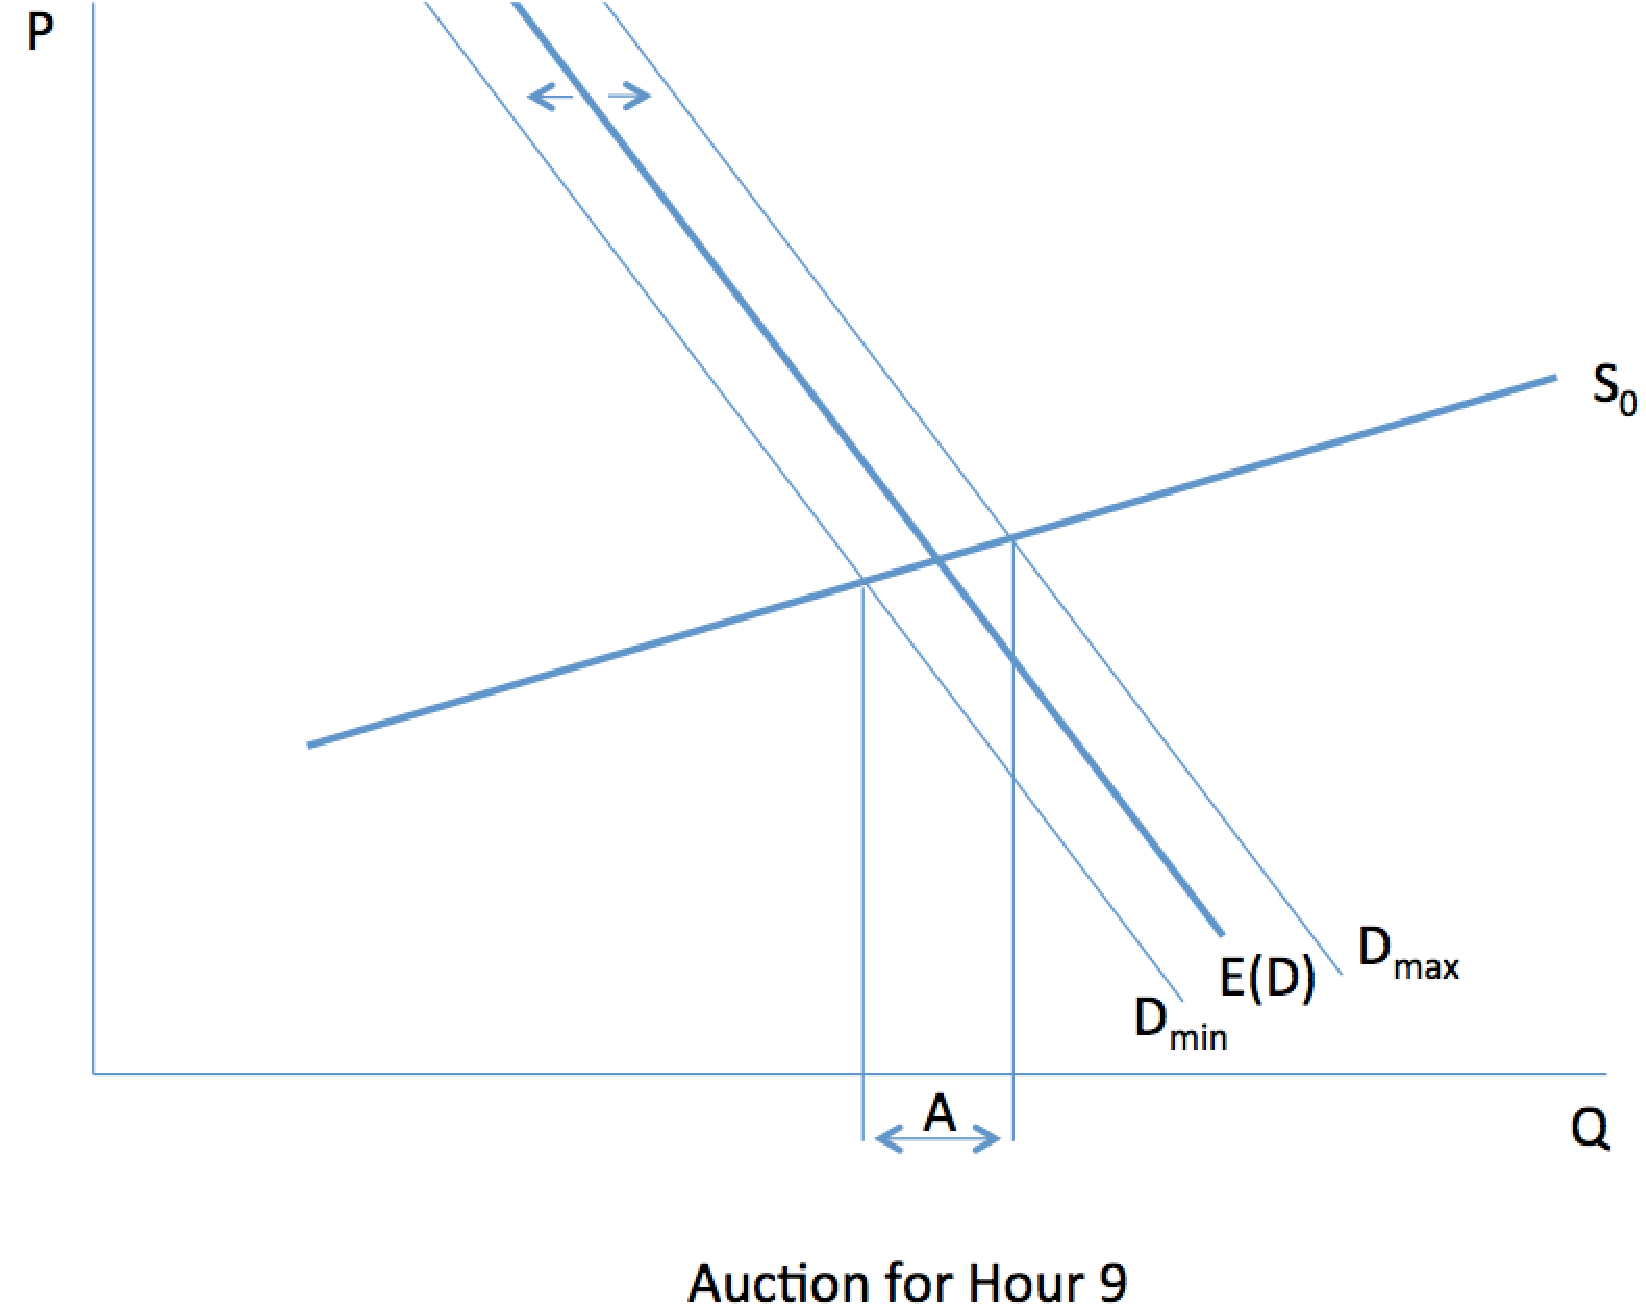
\includegraphics[height=50mm]{figch2/Shot35.pdf} \hspace{0.03cm} 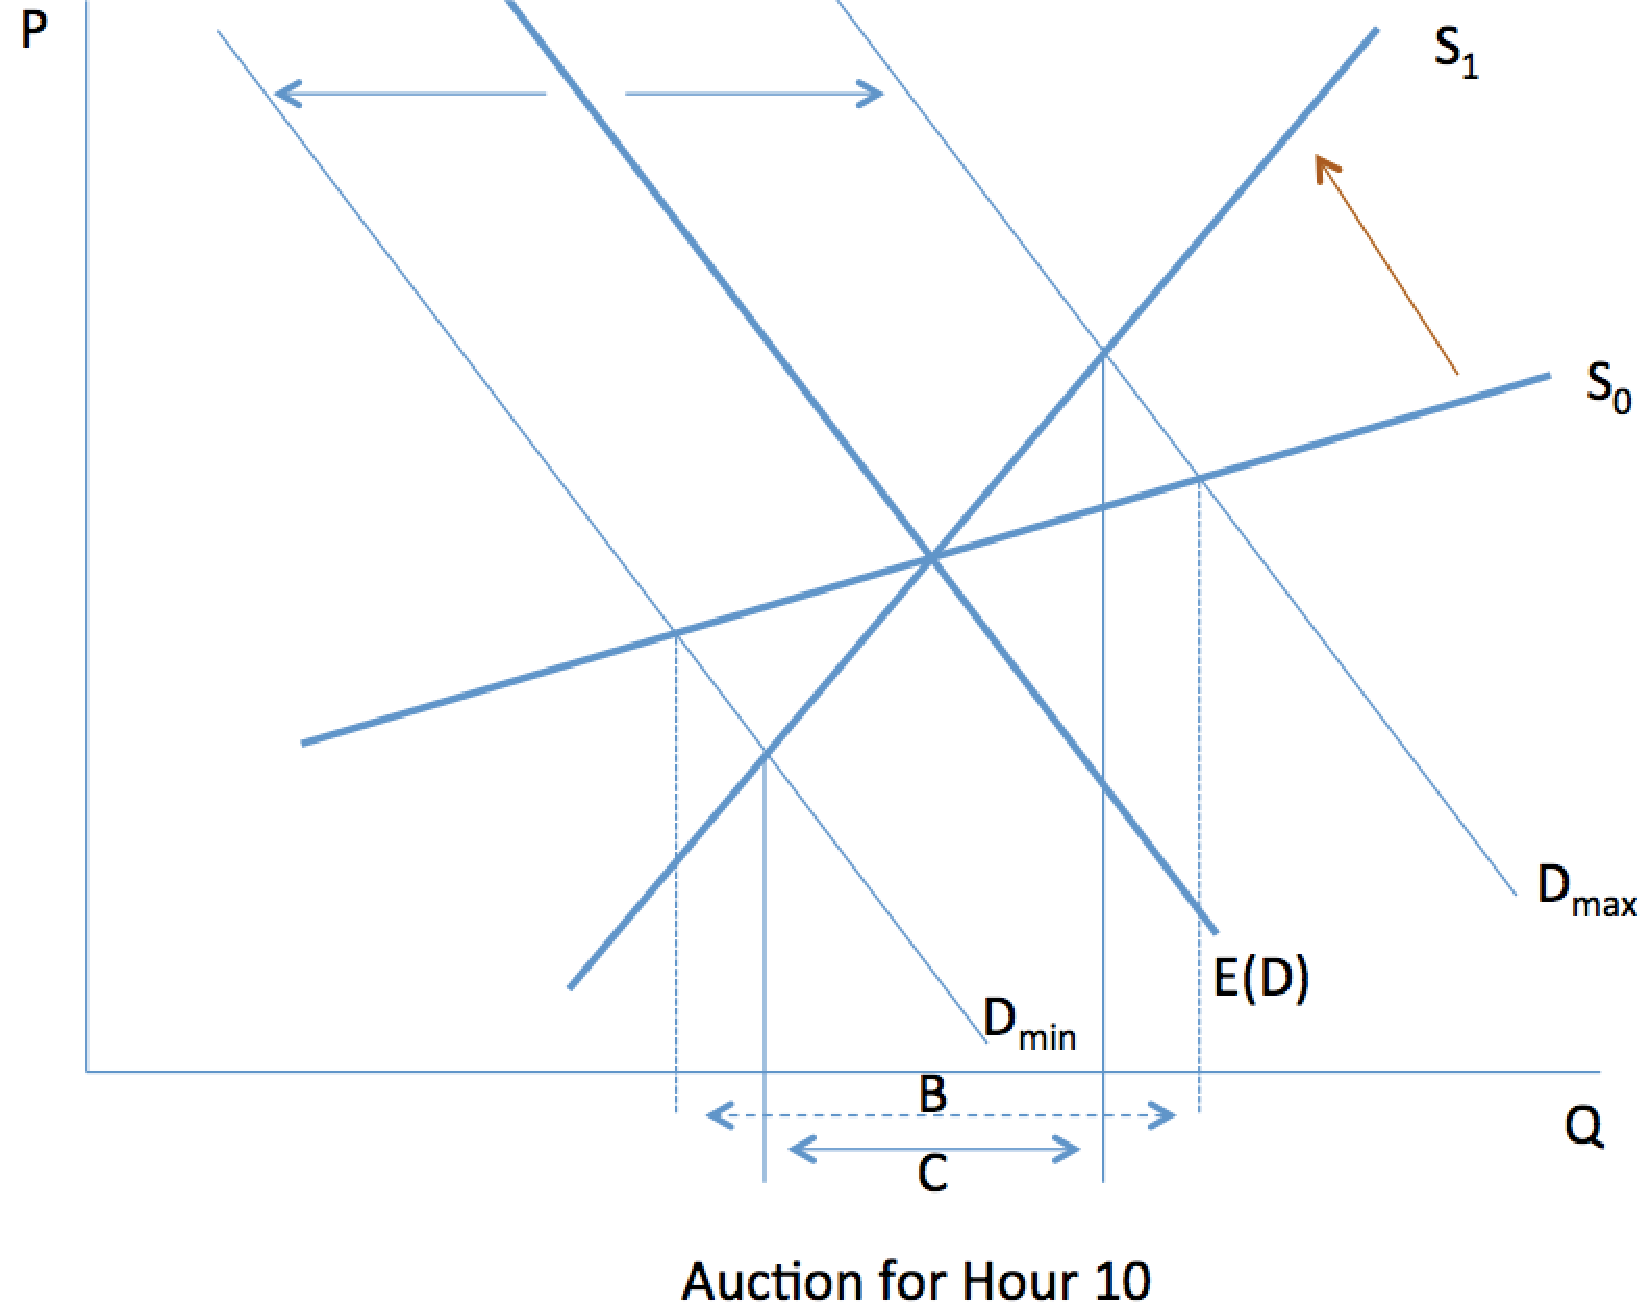
\includegraphics[height=50mm]{figch2/Shot36.pdf} 
} \end{center}
\caption{Illustrating the effect of increased uncertainty.}
\label{predictslope}
\end{figure}

The uncertainty in the market is represented by the width of the envelope of shocks that affect the residual demand function (represented by the arrows on $E(D)$). Thus, in each hour, the residual demand fluctuates between $D_{min}$ and $D_{max}$, where the range between the extremal demands may vary from one hour to the next. \\
 
Before submitting a supply function to the market, the supplier estimates the distribution of probabilities of demand shocks that he will face. In hour 9, the supplier is able to rather precisely predict the realization of the demand function in the auction, i.e. it realises within a tight confidence interval. In hour 10, however, uncertainty in predicting the outcome of the demand realization has grown strongly as represented by the much wider confidence interval on the demand realization. \\

Given a fixed supply bid function $S_0$, the possible range of quantities to be produced by the supplier when going from hour 9 to hour 10 has increased due to the increase in the size of the uncertainty (interval on the Q-axis has grown from length $A$ for hour 9 to the dotted length $B$ in hour 10).\\

Now, we assume that the supplier faces dynamic costs, i.e. it is costly for production to vary on top of any traditional marginal cost consideration and the larger the variation, the larger the cost. Then in the case of a fixed supply bid function ($S_0$ in both auctions), an increase in uncertainty implies an increase in expected dynamic costs. \\

The supplier's reaction to increased uncertainty is therefore to bid a steeper supply function $S_1$ in order to trade-off static optimality and dynamic effects. As a consequence, the range of volumes produced in equilibrium is reduced (the firm produces in the range $C$ instead of $B$). When seen over time, these considerations lead to a smoother production as compared to a constant supply curve: demand shocks are absorbed through a higher price volatility and a lower production volatility. \\

If cautious behavior under high uncertainty is true for all firms on the market and each firm has the same expectation of the probability distribution of the uncertainty, then the reaction of bidding a more price inelastic supply function to increased uncertainty should be observable on the aggregated supply function. \\

We emphasize that this prediction relies on linear demand and supply functions and does not incorporate capacity constraint considerations (both upper and lower bounds on the production volume of plants), which are also important on the market. Furthermore, we have outlined our prediction using a discrete time-setting. The continuous version of this analysis on dynamic costs is explored in detail in chapter 1.\\ 

The present paper tests this mechanism empirically and understands an increase in the slope of aggregate supply bid functions due to an increased level of uncertainty as evidence that firms minimize dynamic costs across auctions. 

\section{The EPEX Spot Market}
\label{epexall}
\subsection{General background}
\label{epexbackground}
The EPEX Spot market is an auction market, which allows firms to trade electricity 12-36h ahead of delivery. It covers France, Germany with Austria and Switzerland. The volume traded on EPEX Spot represents $12\%$, $40\%$ and $30\%$ of the total electricity consumption in these countries respectively in 2013 \cite{epexwebsite1}.\\

The EPEX Spot market has considerably gained in importance over time, and the daily trading volume has almost quadrupled since $2005$, whereas the total electricity consumption has essentially remained constant. The graph in figure \ref{volconsfr} shows these trends very clearly. Furthermore, it shows the significant volatility of the market trading volume (as indicated by the width of the grey-shaded confidence interval).  \\
\begin{figure}[!ht]
\begin{center} \makebox[\textwidth]{
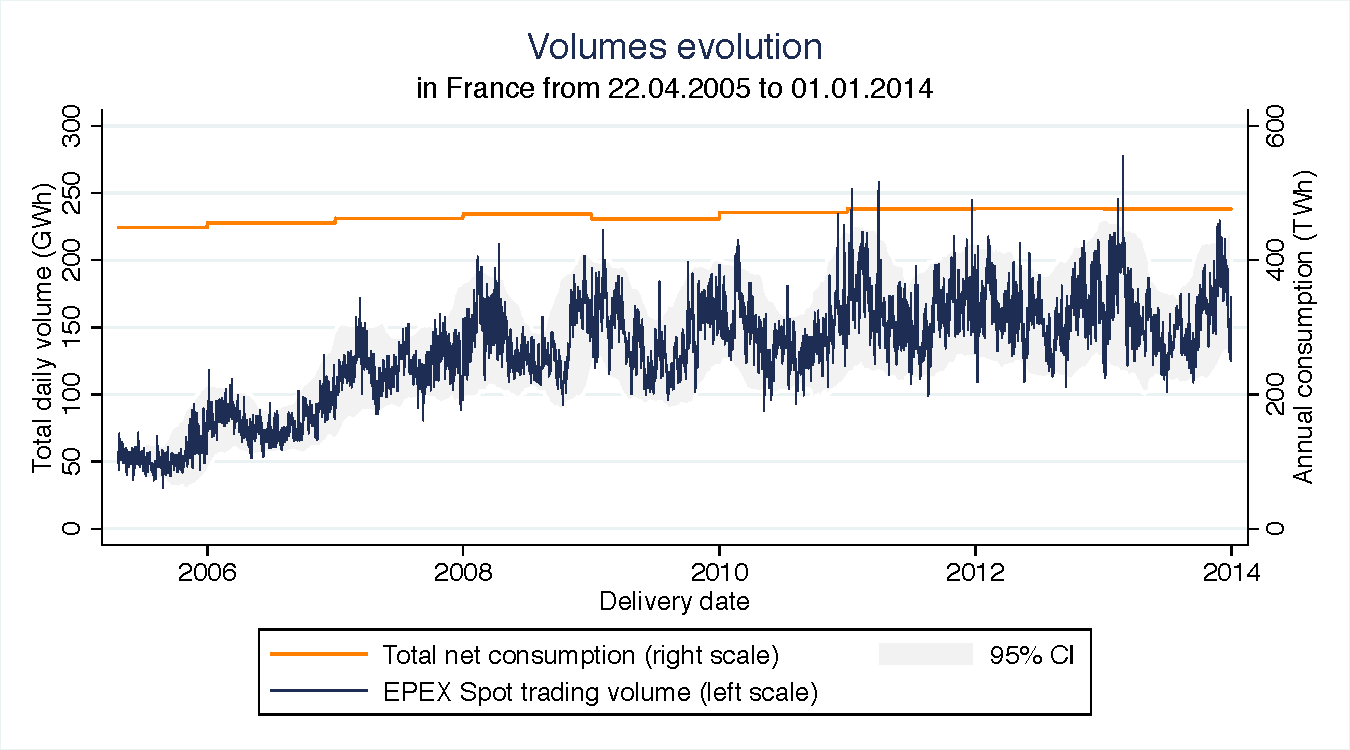
\includegraphics[height=74mm]{figch2/volplusconso3.pdf} 
} \end{center}
\caption{Traded volume plotted against total annual consumption}
\label{volconsfr}
{\small Note: Total consumption is netted of the electricity withdrawal at the level of the production unit. The 95\% confidence interval is based on a 150-days moving window and assumes that volumes are normally distributed in the time window. GWh and TWh stand for giga and terawatt hours, respectively.}
\end{figure}

On the EPEX Spot market, the participants submit supply or demand bid functions to be able to meet their next day's supply commitment. This market is important, because it allows the firms to adjust their portfolio to the upcoming demand. The market matches business to business trades, where producers (the suppliers and transmission system operators) and industrial consumers may participate.\\

The EPEX Spot market settles in a three-headed market that firms use to achieve their desired power position: The long-term bilateral contracting market, the day-ahead market and the intra-day market. Energy cannot be stored, thus a precise power position must be achieved at each point in time. Firms thus face a trade-off between cheap up-front sourcing and costly uncertainty. The closer the market gets to the delivery of its power, the less uncertainty does the firm face in determining its power requirements (pushing firms to wait until the last minute to fill their energy position). However, the imperfect flexibility of the electricity production landscape cannot satisfy the whole demand short-term at a reasonable price, hence firms must anticipate their requirements in order to obtain cheaper power. Consequently, these three markets complement each other to allow firms to gather a power position at a reasonable price. 

\subsection{Auction rules and mechanism}
\label{epexrules}
We present the rules here that applied during the period for which we have data. \\

The EPEX Spot auction occurs daily, all year-round, and proceeds as follows: the order book closes every day at noon for contracts of the following day, results are published two hours later. Bids may be submitted 24/7 from 45 days prior until the closing of the books. \\

Tradable contracts exist for each hour of the day and firms submit an individual bid function for each of these hours, i.e. a separate, simultaneous auction is run for all hours of the following day and trading is specific for each of these hourly tranches.  \\

The bid submission must be a supply function (or a demand function depending on the position of the firm) with at least 2 and at most 256 price/quantity combinations for single contract orders. The final bid function, thus, consists of the explicitly submitted points and all linearly interpolated points between them. The bid curves must be monotonically increasing for a supply function and vice versa for a demand function. Orders are transmitted via an online IT-platform and a redundant confirmation process aims to avoid erroneous bids. Bids are anonymous, and the final electricity distribution is done via the French distribution network controlled by RTE EDF Transport SA.\\ 

Prices are specified in \euro{}/MWh with two decimal digits and must range from -3000\euro{}/MWh to +3000\euro{}/MWh. Quantities are specified in whole MWh. In addition to single contract orders for an individual hour, bidders may submit block orders. \\

These are combined single contract orders with a minimum of two consecutive hours. The vital difference with multiple single contract orders is the "All-or-None" condition, namely that the executions of the individual contract orders forming the block are dependent on one another. That is for a block order covering hours 17 to 20, the quantity demanded for the hour 17 is only awarded if the corresponding quantity is also awarded for the hours 18, 19 and 20. Each registered bidder account is limited to a maximum of 40 block orders per delivery day, each of which is limited in volume to 400 MWh (approx. equal to $0.25\%$ of total daily volume traded on EPEX Spot). \\

The price-quantity determining mechanism is a uniform price, multi-unit auction mechanism: the summed demand and supply curves are computed and the intersection of these gives the equilibrium price and quantity pair.\footnote{\begin{quote}The Auction takes place daily, after the Order Book has closed. The price corresponds to the Matching of Exchange Members' aggregate supply and demand curves of both Single Orders and Block Orders for each Contract. The price determined by the algorithm at the time of Auction is the price at which all Trades will be executed. For price determination purposes, the Exchange Member's interest is assumed to be linear between two price/quantity combinations. The price determination algorithm aims at optimising the total welfare, i.e. the seller surplus, the buyer surplus and the congestion rent including tariff rates. The algorithm determines the execution prices, the matched volumes and the net positions of each coupled market if applicable. It also returns the selection of blocks that will be executed and other complex Orders allowed in other Coupled Markets1 if applicable. The presence of all-or-none Block Orders in the Order Book makes necessary the use of a specific search algorithm, in order to determine a market clearing price.\end{quote} \cite{EPEXRules}} The market clearing mechanism takes into account single and block orders simultaneously and hence solves the corresponding programme by an algorithm of full enumeration of possible solutions, where each partial solution is verified to provide real, compatible prices. The mechanism works under a time limit. In the case of a curtailment, i.e. a disequilibrium with disproportionate prices due to unmatched supply and demand or an abnormal price for a specific hourly contract, the system proceeds to a second price fixing. \\

Of particular interest is the clear distribution of information. Ex-ante bidding, firms in the market know the identities of the rival bidders they face (but neither their individual bid functions nor their results in past auctions), the history of aggregated equilibrium prices and quantities up to that day, their clients' past demand realizations and their individual long term contracting position. Upon the clearing of the market, the aggregated supply and demand bid functions, equilibrium quantity and the equilibrium price become common knowledge. Each bidding account is informed of the contracts it has been awarded, i.e. the individual quantities to be sold and bought through the system.


\section{Our Data Explained}
\label{pschapter}

\label{datasection}
\subsection*{Auction market data}
We have data from the French EPEX Spot market for the period 01.01.2011 to 30.06.2013. This is the latest period, where no significant changes in the auction rules have occurred and where data for all variables can be observed. \\

We observe the full aggregate bid functions for the day-ahead auctions of each hourly contract for both supply and demand. We understand the dataset as a cross-section rather than a time-series\footnote{This is supported by the graph in figure \ref{volconsfr}, which shows a flat total consumption and average trading volume on EPEX Spot since 01.01.2011.} and focus on weekday trading contracts only. This sums up to about 31 500 observations.\footnote{31 500 observations $\approx 2.5$ years of hourly ($*365 *24$) demand and supply ($*2$) functions for weekday trading ($*5/7$).} A single aggregate bid function is the sum of the individual bid functions, which are not available. We also observe the equilibrium price and quantity for each auction. Moreover, we observe the block bidding results at the equilibrium solution only. We ignore the blocked aspects and treat subsequent auctions as independent from one another.\\
	
The two graphs in figure \ref{examplebidfunc} show the aggregate supply and demand bid functions for the same hour of the same day. For a glimpse at the variation of bid functions over time, see figure \ref{graphmultifunc}. The table \ref{overallsummary} sheds some light on the raw data. For further details as well as the plotted distribution of realised market equilibria, refer to appendix \ref{statdes1}. \\

Finally, we reuse the data output from chapter 2. Specifically, we reuse the specific points extracted from the aggregate demand and supply bid functions, which are comparable across auctions. Why these points are useful for our analysis is explained in the methodology section \ref{newapproach}.

\begin{figure}[!ht]
\begin{center} 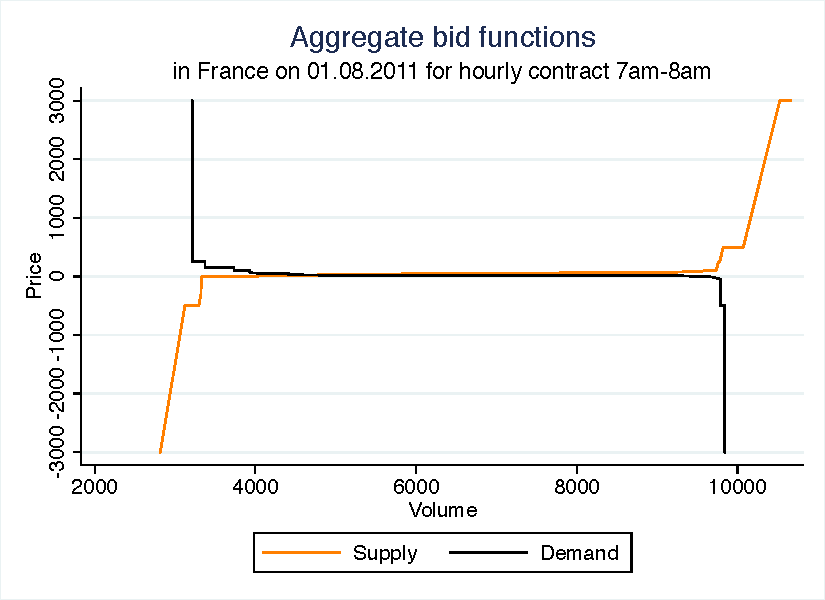
\includegraphics[height=50mm]{figch2/aggbidfuncnozoom.pdf} \hspace{0.05cm}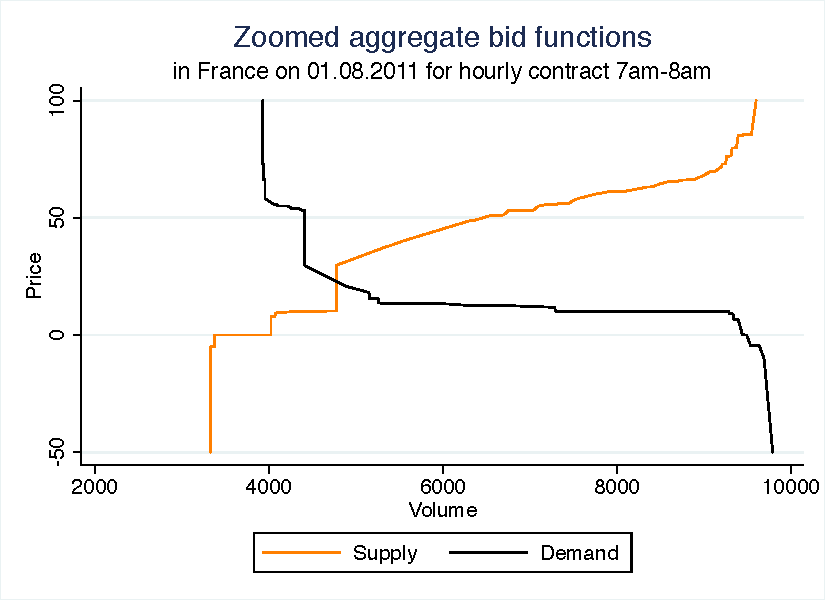
\includegraphics[height=50mm]{figch2/aggbidfuncwithzoom.pdf} \end{center}
\caption{Example aggregate demand and supply bid functions}
\label{examplebidfunc}
{\small Note: The right-hand-side graph is a zoom of the left graph on for the price range  $-50$\EUR{}/MWh  to +100\euro /MWh.}
\end{figure}


\begin{figure}[!ht]
\vspace{0.3cm}
\begin{center}\makebox[\textwidth][c]{
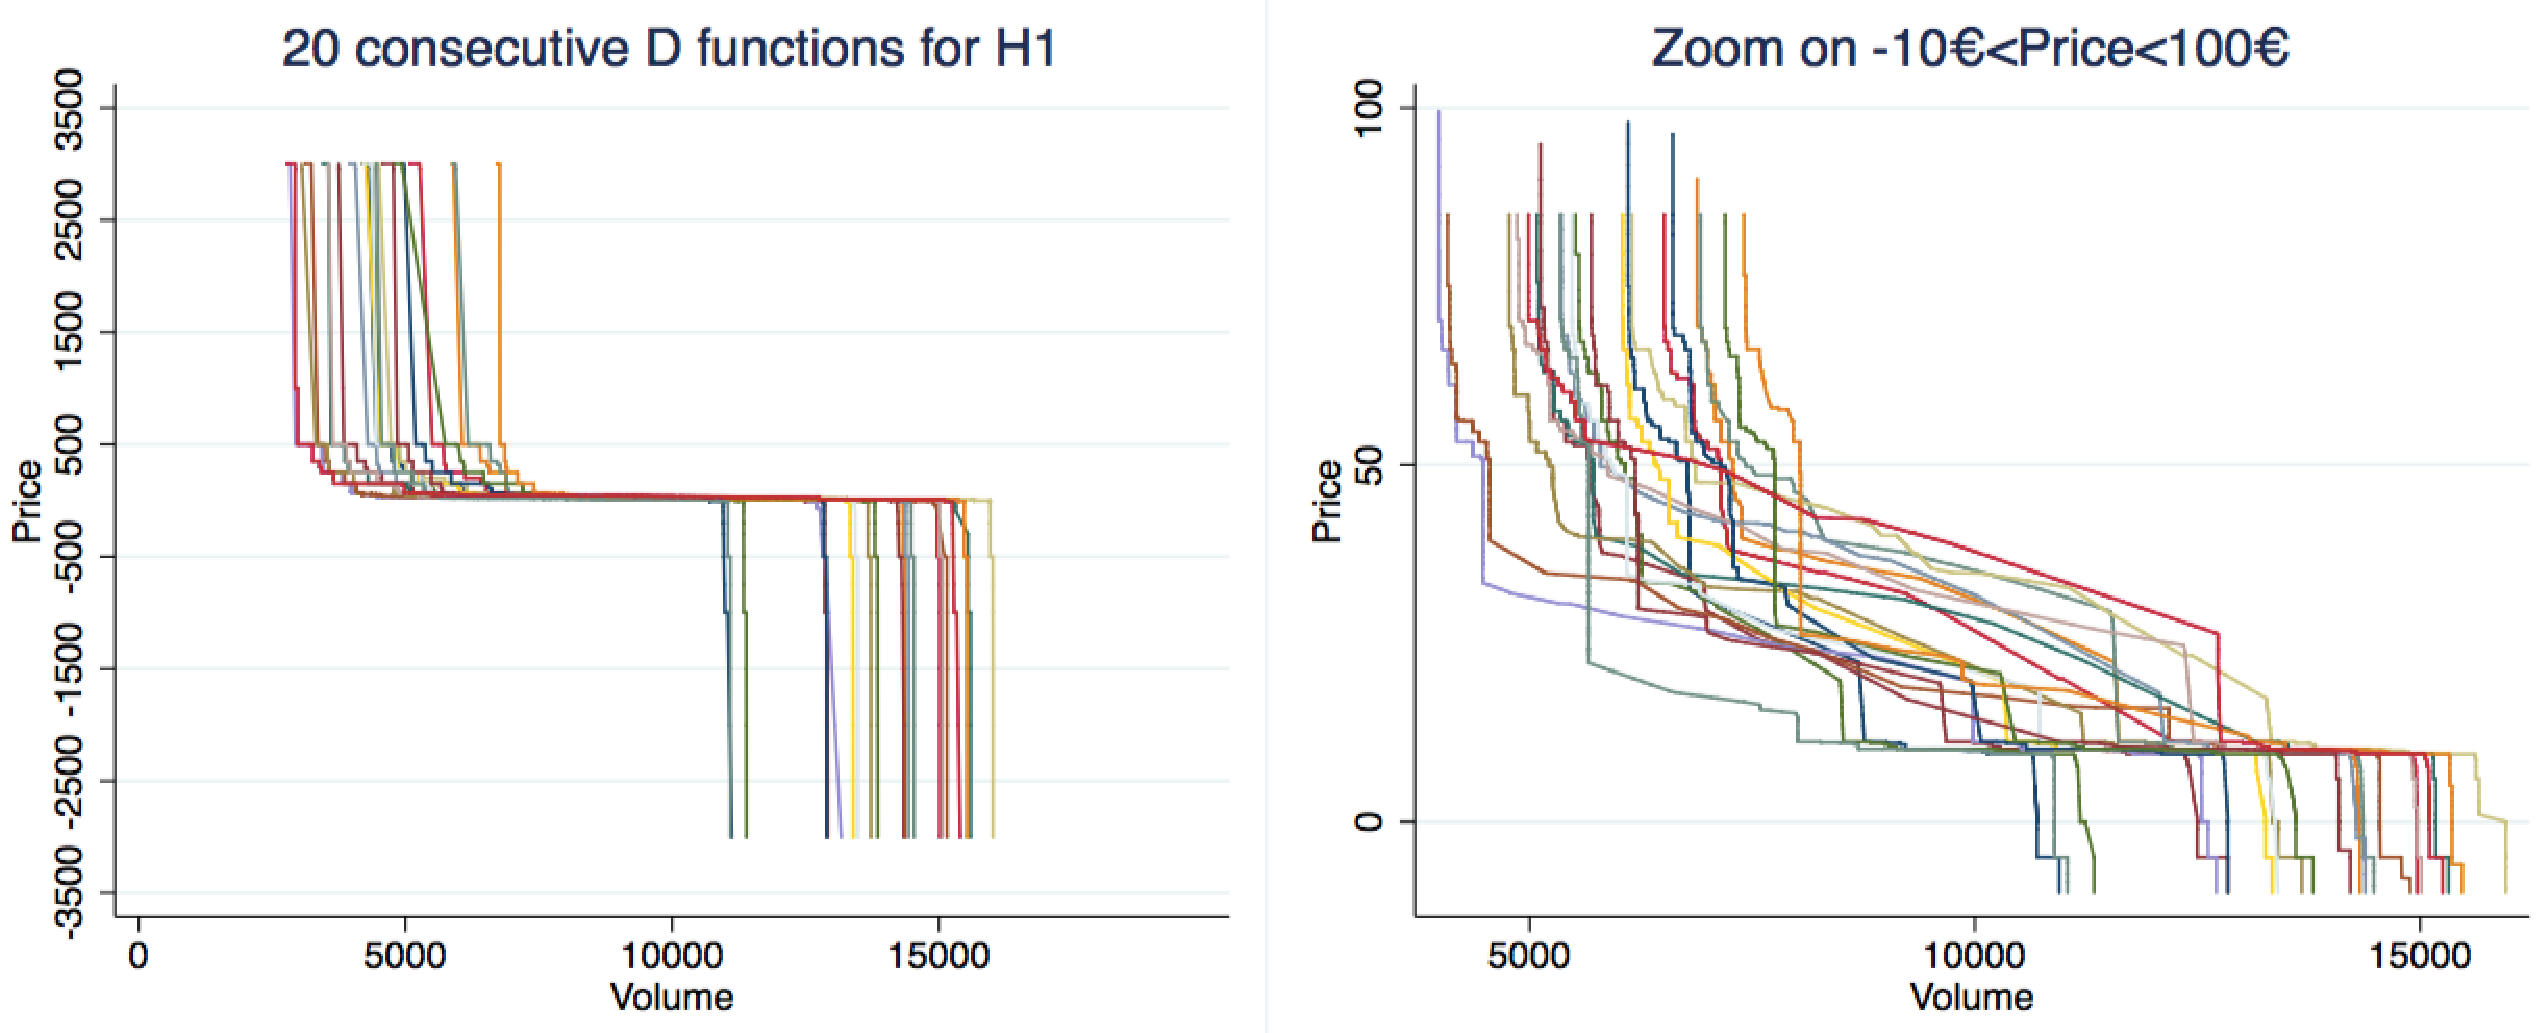
\includegraphics[height=50mm]{figch2/Shot28.pdf}
}\\
\vspace{0.05cm}
\makebox[\textwidth][c]{
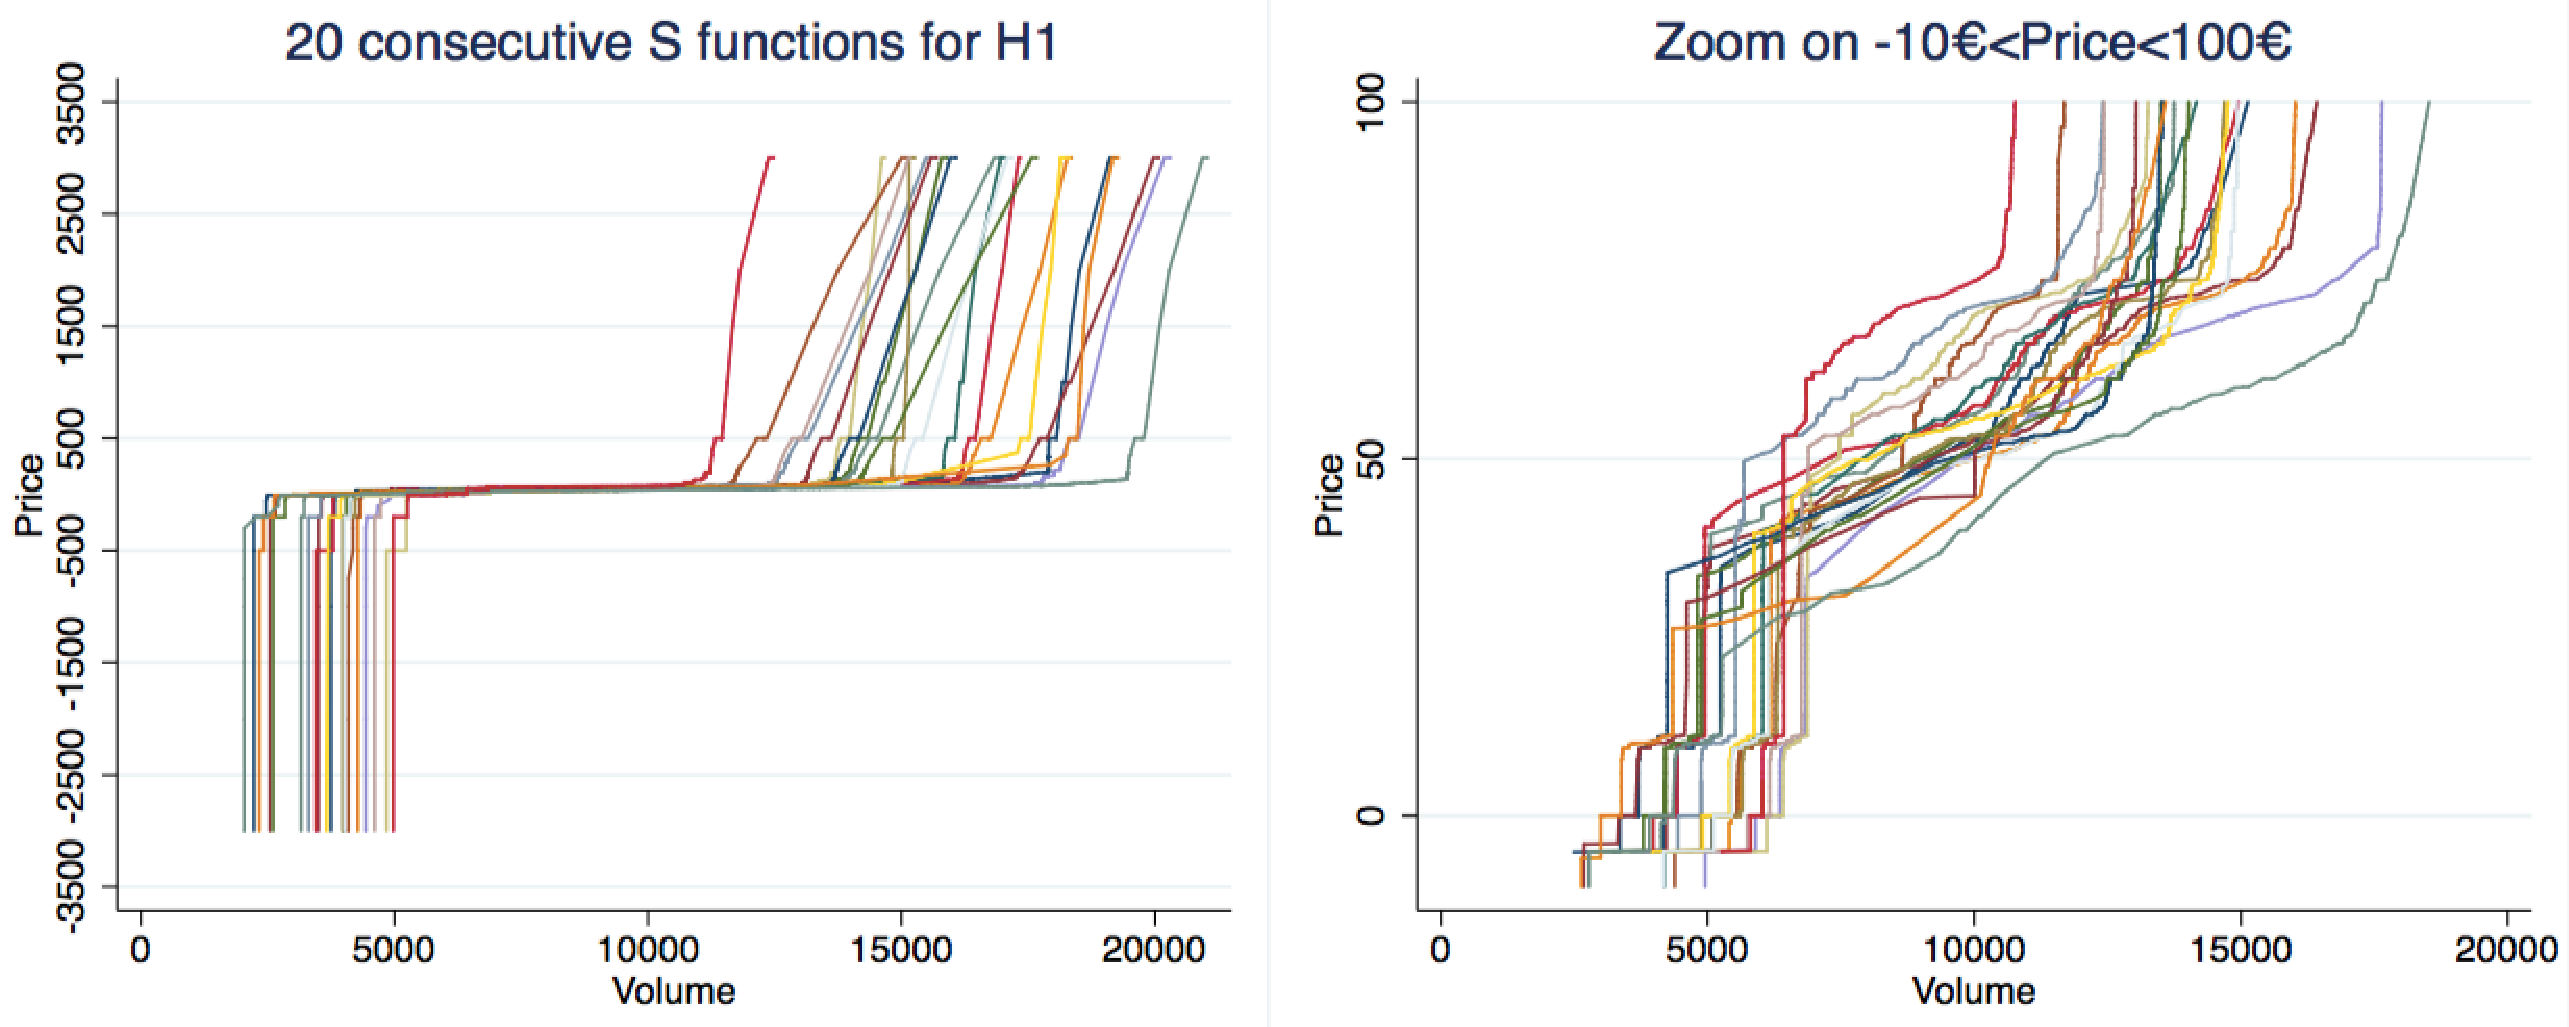
\includegraphics[height=50mm]{figch2/Shot27.pdf}
}
\caption{Aggregate bid functions for 20 consecutive days}
\label{graphmultifunc}
\end{center}
{\small Note: The graph shows 20 consecutive aggregate demand and supply functions for the contracts on hour 1 (between 12 am and 1 am) for the time period 11/12/2011 to 31/12/2011. The graph on the right is a zoom on the price elastic region of the curves on the left.}
\end{figure}

\begin{center}
% matrix: out1 file: /Users/Orie/Cloud/Google Drive - Account henridb1/Encheres Elec/Article/overallsummary.tex   1 Oct 2014 15:48:56
\begin{center}
\begin{longtable}{lrrrrr}
\toprule
 & Mean  & Median  & Std. Dev  & Min  & Max  \\
\midrule
\endfirsthead
\multicolumn{6}{l}{\emph{... table \thetable{} continued}} \\
  & Mean  & Median  & Std. Dev  & Min  & Max  \\
\midrule
\endhead
\midrule
\multicolumn{6}{r}{\emph{Continued on next page...}}
\endfoot
\endlastfoot
Total daily volume &  161,912 &  159,313 & 25,059 & 99,054 &  277,531 \\  
Average realised daily price\footnote{Average price is volume weighted over the 24 hourly contracts of the delivery day.} &    46.6 &    48.3 &    17.2 &   -39.0 &   381.2 \\  
%Congruence ratio\footnote{It is defined by the ratio of maximum supplied volume to maximum demanded volume. It is based on \cite{armstronggalli2007empirical} and measures liquidity in the market by comparing how similar buyer and seller attitudes to trade are on the market. The authors find that unusually high prices generally occur when this metric exceeds 2.} &     1.11 &     1.07 &     0.32 &     0.45 &     4.51 \\  
Minimum demanded agg. volume\footnote{Minimum and maximum volumes for both demand and supply refer to the aggregate volume bid on the market for a single hour contract at the extremal prices of $+3000$\euro /MWh or $-3000$\euro /MWh.} & 5,030 & 4,968 & 1,467 &   914 & 11301 \\  
Maximum demanded agg. volume & 13,327 & 13,222 & 2,212 & 4,990 & 23,254 \\  
\midrule
Minimum supplied agg. volume & 3,721 & 3,526 & 1,344 &   618 & 10594 \\  
Maximum supplied agg. volume & 14,390 & 14,142 & 3,051 & 6,580 & 35,356 \\  
Bid points per demand function &   543 &   531 &   163 &   115 & 1,253 \\  
Bid points per supply function &   640 &   632 &   143 &   184 & 1,283 \\  
Bidders per auction\footnote{Due to the anonymity of the auction procedure, it is unknown which bidders submitted bids. Consequently, it cannot be deduced how many bid steps a typical bidder submits. Number of registered bidders for the French EPEX Spot market as of 01.10.2014.} &   - &    - &   - &   1 & 101 \\
\bottomrule
\caption{\label{overallsummary} Some descriptive statistics}
\end{longtable} 
\end{center}
\end{center}


\subsection*{Exogenous factors}
Regarding weather statistics, we have hourly previsions for temperature, wind and cloudiness from the GFS (Global Forecast System) as well as hourly observations for these quantities and luminosity from M\'{e}t\'{e}oFrance
. The previsions from the GFS are in the form of weather maps that are outputted from simulations that run one-day ahead at 6 am. This is the weather information that market participants have access to when bidding on EPEX Spot.\footnote{The next weather simulation run takes place at 12 noon and is therefore not being used by the bidders on the EPEX day-ahead market, as the deadline for submitting bids is precisely 12 noon.} The weather observations are in the form of tables for specific weather stations (between 100 and 200 depending on the specific parameter of interest).\\

Moreover, we have the location of the total installed capacity per generation type (i.e. wind turbines, solar panels, etc.) at the level of the postcode, that is roughly a 3km precision. We obtain this data from the SOeS, a branch of the French government producing data on environmental issues at large. \\

Population data and data on the level of the domestic production from the manufacturing industry is obtained in monthly steps from the French National Institute of Statistics and Economic Studies (INSEE). From the same source, we obtain the spot prices for petrol and natural gas as well as the import prices at the border for coal, which we use as a proxy for the domestic prices. Prices for the European CO2 emission certificates are taken from the Portuguese secondary market (SENDECO$_2$) for European Unit Allowances (EUA).\footnote{Each unit EUA permit allows one tonne of CO2 emissions.}\\

As a very coarse proxy for generation from hydro power plants, we have the total weekly stock of water in domestic dams (in the form of the summed height of all dam water levels in France) from RTE the grid operator.


\section{Methodology}
\label{newapproach}
We want to identify the impact that the level of uncertainty has on the price elasticity of the aggregate supply function. In data terms, this means that we aim to regress the slope of (aggregate) supply bid functions on a proxy corresponding to the uncertainty that existed at the time of bidding. The uncertainty may come from two different sources: (i) uncertainty about the realization of market demand and (ii) uncertainty on the generation from renewables. Both types of uncertainty affect the residual demand curve faced by each supplier.\footnote{Renewable generation benefits from a feed-in guarantee on the market and thus reduces the residual demand for all traditional electricity producers.}\\

This regression is able to explain how supply firms adjust their bidding strategies to the expectation of demand shocks that they face. Statistical significance of the level of uncertainty on the slope of the supply function would be evidence that firms take the strategic considerations of dynamic costs into account. \\

\label{strat}

First, in section \ref{identification} we show the final regression of interest. Sections \ref{LHS} and \ref{RHS} then detail the theory and empirics underlying the variables that feed into the final regression. \\

Some of the information used in our analysis is drawn from the bid functions of the EPEX Spot market. As introduced in section \ref{datasection}, we observe the full aggregate bid functions for both supply and demand, the shape of which (and thus the information that we aim to extract from them, e.g. their slope) varies differently at different points (recall the graphs in figure \ref{graphmultifunc}). \\

Generally speaking, a regression aims at quantifying the impact of some independent variables on a dependent one. The dependent variable is most frequently numerical, and the independent variables explain part of its value. Here the dependent variable is functional in nature, that is that we aim to describe how the supply function changes shape with respect to some independent variables. One observation is formed of one function coupled to the value of some independent variables. We therefore adopt a functional data analysis approach, which allows us to condition our analysis at specific points $k=1,..,K$ of the functions. This approach allows us to define comparable points across auctions, that is different functions, in order to derive insights. \\

More precisely we want to quantify how uncertainty affects the strategy of bidders from one hour to the next. For this we cannot rely on a standard estimation of the overall demand or supply functions from market outcomes, we want to actually measure how the functions that we observe change shape. \\

The methodology to select comparable points across auctions is detailed in chapter 2. This appendix also evaluates the results when applying the technique to our data from the EPEX Spot market. Figure \ref{TypeallocK} shows the selected points on an exemple of demand and supply curve. \\

The different types of points selected capture different information of the aggregate bid functions. The most important point is the one we label $k=3$, which corresponds to the central part of the bids. This point is most relevant for equilibrium determination.\footnote{See figure \ref{g7f} for a glimpse at the distribution of equilibrium outcomes.} The points $k=2,4$ are the points of maximum curvature and represent the transition points between the central (very price elastic) region and the outer (very price inelastic) regions of the bid function. Last, we have the points $k=1,5$ which are imposed by the auction rules and are the endpoints of the bid functions. \\

\begin{figure}[!ht]
\begin{center} 
\makebox[\textwidth]{
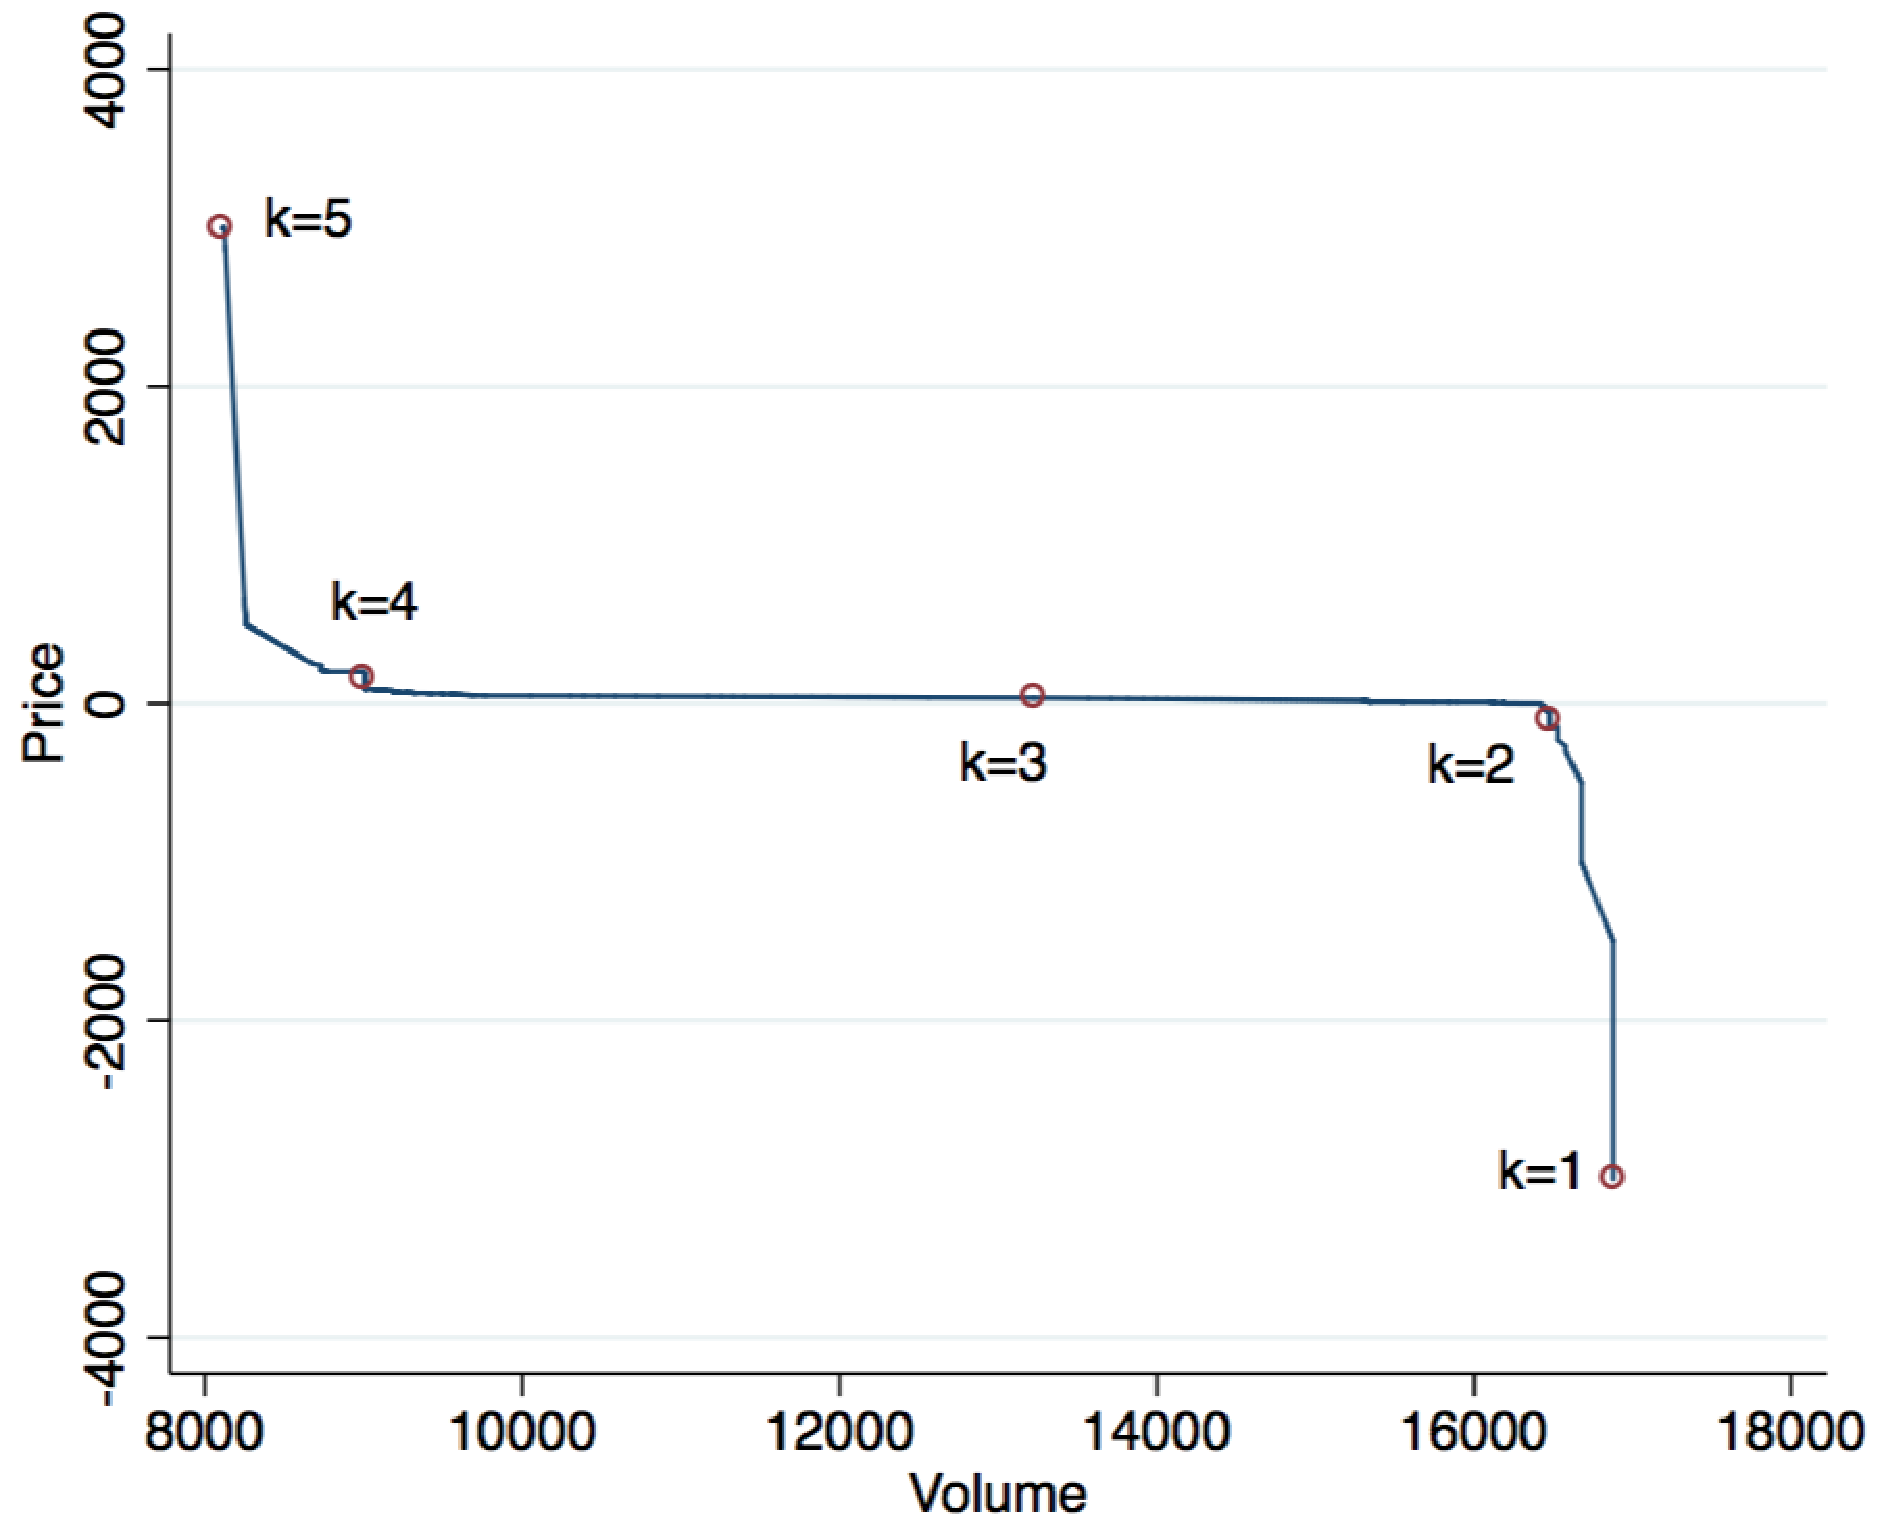
\includegraphics[height=50mm]{figch2/DemandplusK.pdf} 
\hspace{0.05cm}
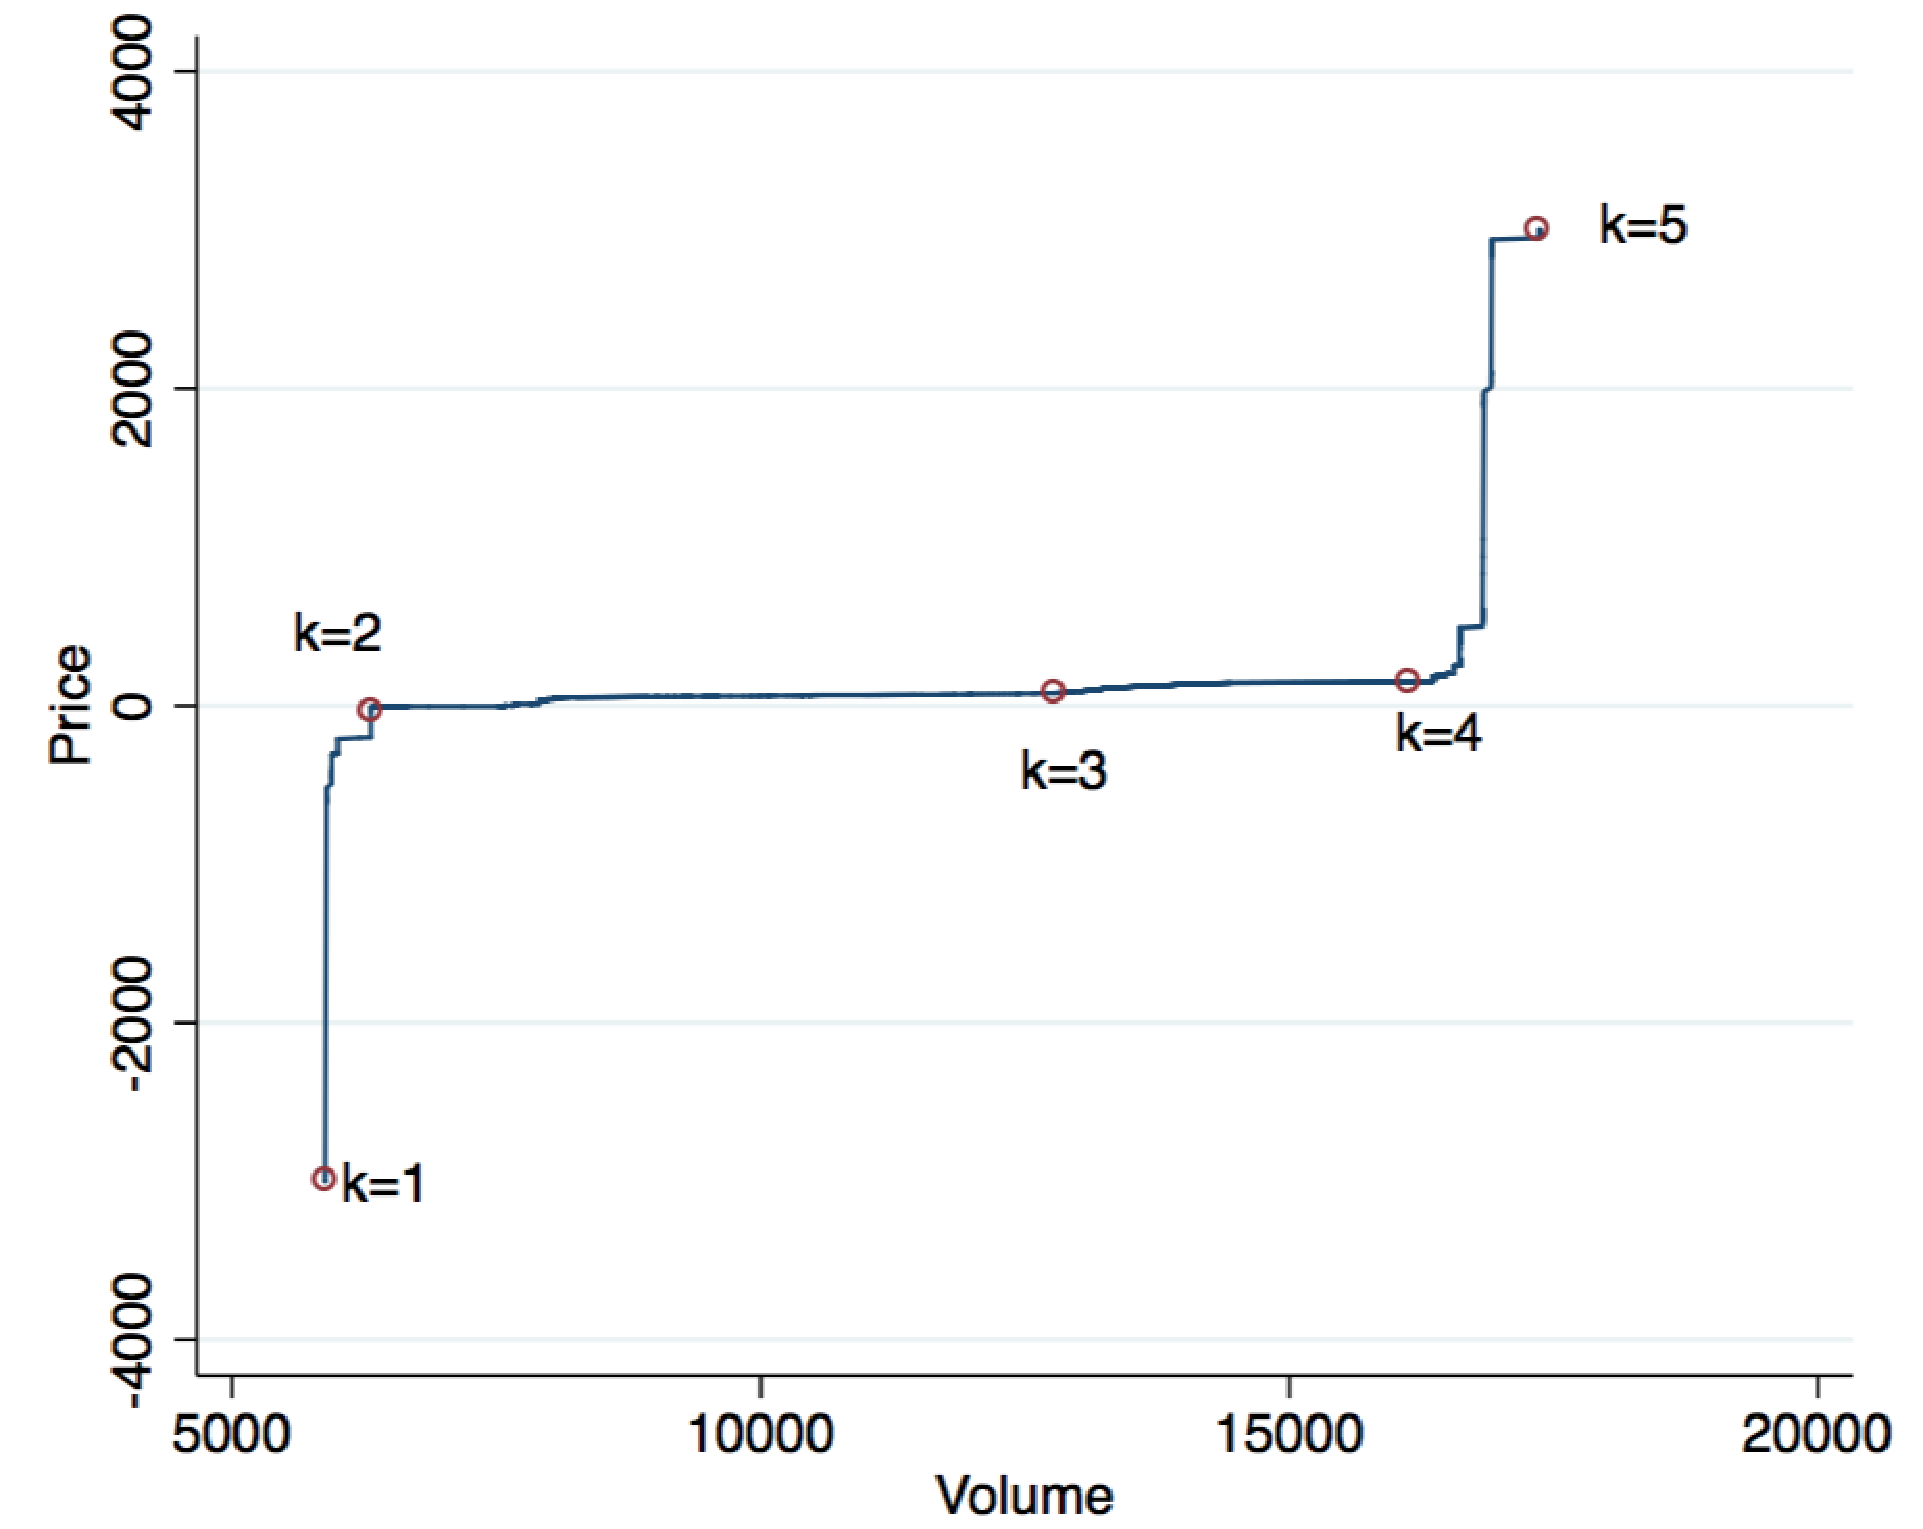
\includegraphics[height=50mm]{figch2/SupplyplusK.pdf} 
} 
\end{center}
\caption{Selected points on original bid functions}
\emph{Note: } The demand function left, the supply function right, the graph superposes and names the points selected according to the methodology of section \ref{newapproach}.
\label{TypeallocK}
\end{figure}
 
In chapter 2, we also detail the choice of setting $K=5$ and show that this choice allows us to improve the precision of our analysis by a factor of 50 when it is conducted on the 5 points simultaneously.\footnote{We briefly mention that the evaluation of the point selection has revealed focal price points for the points $k=2,4$. These points are however rarely relevant for equilibrium determination.}

\subsection{Regression methodology}
\subsubsection{Identification}
\label{identification}
At each of these comparable points, we want to identify the effect of uncertainty on the slope of the supply function. \\

Defining $S'_{i,k}$ the slope of the supply function of auction $i$ at point $k$ in the quantity (X-axis) - price (Y-axis) dimension, $\boldsymbol{X^S}$ being the vector of exogenous variables, PLU$^D_{i,k}$ being the proxy for the level of demand uncertainty, PLU$^R_i$ being the proxy for the level of uncertainty from renewables, what we called the width of our possible shocks in the first chapter, $\alpha$ being the regression constant and $\epsilon$ being the error term, we estimate the following:
\begin{eqnarray}
\label{secondstagereg2}
S'_{i,k} =\alpha_{k}^S+ \beta_{k}^S \text{PLU}^D_{i,k} + \gamma_{k}^S \text{PLU}^R_{i} + \boldsymbol{\delta_{k}^S X^S_i}+\epsilon_{i,k}^S
\end{eqnarray}

We are interested in the sign and magnitude of the coefficients $\beta^S$ and $\gamma^S$, which identify the effects of the PLUs (PLU$^D$ and PLU$^R$, respectively) on the shape of the supply bid function. From the predictions outlined in section \ref{intropredict}, we expect a positive coefficient when uncertainty levels increase.\footnote{Specifically, we want $\beta^S$ to be positive, $\gamma^S_1$ positive and $\gamma^S_2$ negative. For details on $\gamma^S$, see section \ref{proxyautocorrel}.}\\ 

\subsubsection{Left-hand-side variables}
\label{LHS}
We extract the slope of the aggregate supply function at any given point $k$ from a kernel density estimation with a bandwidth of 45 units.\footnote{The slope is a by-product of the point selection mechanism, and the bandwidth selection for the smoothing thus follows the same considerations as for the latter. The details of this choice are specified in chapter 2.}  \\

Effectively, this is a smoothed version of the slope. This makes our slope estimates robust to steps in the bid function\footnote{In our data, we observe that bid functions are effectively step functions. On EPEX spot $256$ price-quantity combinations are allowed per bidder. When additional bid points are costly, then stepwise bidding behaviour may be very different from a setting where continuous functions can be bid \cite{kastl2011discrete}. Due to the fact that, on average, we do not observe that firms use up all available price-quantity combinations, the cost argument of an additional bid point seems weak. Hence, by smoothing the slope we approximate the unconstrained, continuous bid function. }, which in turn allows us to test the predictions from the theoretical paper. Steps in the bid functions mostly are much larger towards the extremities of the bid functions and probably arise from capacity constraints considerations. Working with smoothed slopes is in line with previous work \`{a} la \cite{pw2002etude} and \cite{ozcan2004logistic}, who also apply reduced form models to aggregate bid function data. 

\subsubsection{Right-hand-side variables}
\label{RHS}

We are regressing an ex-post measure of the auction market (realised slope of the supply bid function) on ex-ante information that bidders have at the time of bidding, i.e. which is available at midday of the day ahead of delivery.  
We thus keep a strict separation of the ex-post and ex-ante information to the left and right hand side of equation \ref{secondstagereg2}, respectively. This separation allows us to circumvent endogeneity problems and validates the use of simple OLS regressions. \\

For this reason, we construct our PLUs on the basis of predicted uncertainty. However, for data availability reasons we cannot exclude endogeneity problems completely. For details, see the discussion in section \ref{endogeneityconcern}.  \\

In this subsection, we first outline how we generate the proxies for the level of market demand uncertainty (PLU$^D$) in section \ref{proxyunc}. Second, we construct the proxies for the level of uncertainty from renewables energies (PLU$^R$) in section \ref{proxyautocorrel}. Third, we detail how the vector of exogenous variables ($\boldsymbol{X}$) is constructed in subsection \ref{controlssec}.  \\

\subparagraph{Generating proxies for uncertainty from market demand (PLU$^D$)}
\label{proxyunc}

We construct a proxy for the level of the demand uncertainty (PLU$^{D}$) by using the residuals from a demand estimation on exogenous parameters as a measure of the uncertainty that bidders face in an auction. Specifically, our PLU$^D$ is the expected squared level of the prediction errors that firms expect to make when anticipating the demand level of the day ahead. We assume that the ex-post prediction errors give a reasonable estimate of the uncertainty at the time of bidding. \\

The uncertainty proxy is obtained as detailed next in a three-step procedure. In the first step, we explain what kind of uncertainty our PLU$^D$ refers to. The second step details the conceptual details of constructing the PLU$^D$. The third step computes the PLU$^D$.

\subparagraph{In the first step,} 
\label{firststepresiduals}
we focus the analysis to a fixed number $K$ of comparable points across auctions by using the non-parametric point selection technique outlined in section \ref{newapproach}. Each k$^{th}$ point is defined by a price and a quantity, which we regress independently on the exogenous variables. \\

Let us call $P_{i,k}^D$ and $Q_{i,k}^D$ the price and quantity of point $k$ of the realised demand function in auction $i$, $\boldsymbol{X^D_i}$ the vector of exogenous variables relevant for the demand estimation.
\begin{eqnarray}
P_{i,k}^D=\alpha_{k}^{D,P}+{\boldsymbol{\beta_{k}^{D,P}}} \boldsymbol{X^D_i}+\epsilon_{i,k}^{D,P} \label{regDP}\\
Q_{i,k}^D=\alpha_{k}^{D,Q}+{\boldsymbol{\beta_{k}^{D,Q}}} \boldsymbol{X^D_i}+\epsilon_{i,k}^{D,Q} \label{regDQ}
\end{eqnarray}
In regressions \ref{regDP} and \ref{regDQ}, firms try to anticipate the realization of the demand using the exogenous information available. We consider that the producers are able to do such an analysis at the time of bidding. \\

The prediction errors  $\epsilon_{i,k}^{D,J}, \; J=\{Q, P\}$ are a consequence of the stochastic nature of the demand and hence a manifestation of the uncertainty. We consider that more uncertainty will lead to larger prediction errors being made in equilibrium and adopt the square of the residuals $ \bigl( \epsilon_{i,k}^{D,J} \bigr)^2$ as our measure for the realised level of demand uncertainty.

\subparagraph{In the second step,} 
\label{secondstepresiduals}
we recover the residuals from the demand estimation in regressions \ref{regDP} and \ref{regDQ} and test for heteroskedasticity using \cite{white1980heteroskedasticity}, which is clearly confirmed (see tables \ref{VolDEPur52} and \ref{PriceDEPur52}). \\

Heteroskedasticity means here that the variation of error terms varies conditional on the levels of the exogenous factors: $E(\epsilon_i^2 \vert \boldsymbol{X_i})=g(\boldsymbol{X_i})$. However, they are still orthogonal: $E(\epsilon_i \vert \boldsymbol{X_i})=0$, thus ensuring that the prediction is unbiased, but not ``best" in the sense of the best linear unbiased estimator (BLUE). Thus, heteroskedasticity results in inefficient regressions where the estimator is not minimum variance. Since we do not interpret regressions \ref{regDP} and \ref{regDQ} for causality, but only for predictive purposes, we stick to the unbiased OLS. \\

The heteroskedasticity regression is given for $J=\{P,Q\}$ by
\begin{equation}
\label{heteroskedeqn}
 \bigl( \: \epsilon_{i,k}^{D,J}\: \bigr)^2= \alpha^{U,J}_{k} + \beta^{U,J}_{k} \boldsymbol{X^D_i} 
 +\epsilon^{U,J}_{k}
\end{equation}

\subparagraph{In the third step,} we compute the predicted PLU$^D_{i,k}$ that firms use when bidding in the auction as:
\begin{equation}
\label{predictu}
 \underbrace{ \widehat{ \bigl( \: \epsilon_{i,k}^{D,J}\: \bigr)^2}}_{\widehat{\text{PLU}}^D_{i,k}}= \alpha^{U,J}_{k} + \beta^{U,J}_{k} \boldsymbol{X^D_i} 
 % +\epsilon^{U,J}_{k}
\end{equation}
The idea is that by experience, firms in the market know that their predictions are more or less accurate depending on the environmental conditions (in the sense of realizations of exogenous factors). In other words, firms can use the realizations of $ \boldsymbol{X^D}$ to infer the accuracy of their demand predictions. Technically speaking, they can use the heteroskedastic nature of the residuals to forecast the level of uncertainty that they face.\\

The PLU$^{D}$ subs into regression \ref{secondstagereg2}. 
For simplicity, we do not include the uncertainty proxies PLU$^D_{i,k}$ measured at all $K=5$ points in regression \ref{secondstagereg2} simultaneously, but only a single PLU$^D_{i,k}$ at a time. 
Therefore in the final regression \ref{secondstagereg2}, we regress the slope at a point of the supply function on the PLU$^D_{.,.}$ estimated at the corresponding point on the demand function. The pairing is done in the quantity dimension. This means that the slope of the supply function at point $k=2$ is regressed on the uncertainty measured at point $k=4$ of the demand function (recall the labelling of the points as given in figure~\ref{TypeallocK}). We indicate this quantity paring in the index $k^{-1}$ of the PLU:
\begin{equation}
\label{levelproxy}
\text{PLU}^D_{i,k} = 
\widehat{\text{PLU}}^D_{i,k^{-1}} 
%= \bigl(\widehat{\epsilon}^D_{i,k^{-1}}\bigr)^2 
\end{equation}
An increase in PLU$^D_i$ corresponds to an increase in the uncertainty about the market demand realization. We thus expect $\beta^S$ to be positive in regression \ref{secondstagereg2}.

\subparagraph{Generating proxy for uncertainty from renewable energies (PLU$^R$)}
\label{proxyautocorrel}

We have already referred to the statement that the intermittency of renewables causes large residual demand shocks \cite{epexwebsite1}. Suppliers are thus wary of the expected production of renewables generation. \\

Given that renewable generation is an exogenous source of supply and is completely injected on the network without being bidden for (fixed feed-in tariff), it affects the residual demand curve for each supplier, but does not enter the PLU$^D$, which captures the uncertainty on market demand only. \\

In predicting the generation from renewables, we assume that suppliers are able to infer renewables generation from meteorological forecasts.\footnote{We specify the technique in chapter 2 and use it to construct our controls in section \ref{controlssec}.}\\

When forecasting the residual demand shocks due to generation from renewables, we consider that suppliers have an idea of the precision of their estimate based on the ``look" of the meteorological forecasts that they have. By look, we mean the geographical heterogeneity or homogeneity of the forecasts, i.e. if when looking at a weather map, one sees a lot of spatial variations or not. \\

We consider that this notion of geographical heterogeneity of the forecasts correlates to the uncertainty associated with the prediction of renewable production. The argument is as follows: \\

\textbf{First}, renewable production is built by aggregating the forecast of all individual renewable sources. This means knowing the position and capacity of every renewable source, querying weather forecasts for all of these points, modeling the renewable's response to the forecasted weather and adding the forecasted productions. \\

\textbf{Second}, we note that weather is spatially correlated, which means that the closer two points are, the closer the values for a given weather variable (the air temperature at your left hand is very close to that at your left hand, but less so across the city, and even less so across the country). This correlation roughly follows an exponential law: the difference between the values of a weather variable between two points behaves in a linear fashion for small distances and saturates at large distances.\footnote{Intuitively, the characteristic lengthscale of autocorrelation represents the distance required between two geographical points on a map of weather forecasts to observe a decorrelation of half of its maximum value. For example on the wind speeds prediction, a characteristic length of 80 km means that if we observe two very distant points (say 1000km) to have a difference in wind speeds of, on average, 50km/h (this being the maximum difference, we are in the saturated regime), then we will observe, on average, wind speed differences of 25km/h for points distant from each other by 80km.} The transition between those two regimes is given by a characteristic lengthscale, a bit less than 200km on average. \\

\textbf{Third}, we observe that the average distance between production points is large enough that the relevant regime of autocorrelation is the saturated part.\footnote{For N production points, we compute the N(N-1)/2 pairs of points, consider their distances and compute the average of these distances weighted by the production capacity at every point. In the case of the wind, we have an average distance of 459 km, in the case of the photovoltaic production we have an average distance of 499km.} \\

\textbf{Fourth}, we note that there are two main channels through which the overall uncertainty about renewable production is related to the weather. There is an issue of error averaging, which means that if the weather becomes very spatially uncorrelated, one can expect errors to cancel out relative to a given bias in the forecast. This channel would tend to imply that more spatial variations imply a smaller uncertainty about production. There is also the issue that weather forecasts are numerical simulations and that the mesh size for such simulations, typically 5km for the high precision ARPEGE model of Météo France, implies that the errors are higher as the simulated phenomenons have higher gradients. This means in our case that the uncertainty about the forecast increases as the weather becomes more spatially uncorrelated. \\

\textbf{Fifth}, these two effects are of opposite signs, but our third point is an argument for considering that the averaging of errors is smaller than the simulation errors. Therefore, we expect our uncertainty to increase as the spatial autocorrelation decreases (i.e. more spatial variation). \\

This can be summed up with the following hand-waving argument: when there is more spatial variations, the weather is more messy, therefore more difficult to predict. \\

We compute this characteristic lengthscale ($L$) as described in chapter 2. Our PLU$^R$ is defined as the two proxies 
\begin{align}
 \text{PLU}^R_{1,m} &= \frac{1}{L_m}, \quad \quad  \text{where } m=\{\text{Wind, Solar, Temperature}\} \\
  \text{and }  \quad \text{PLU}^R_{2,m} &=  \bigl(\frac{1}{L_m}\bigr)^2
\end{align}

As explained above, we expect firms to face less uncertainty in predicting weather conditions when the lengthscale of autocorrelation $L$ is longer since the overall weather conditions will be more homogenous. A longer length $L$ (less uncertainty), will yield a smaller PLU$^R$ and we expect a flattening of the supply curve. I.e. we expect a positive coefficient $\gamma^S_1$ on the PLU$^R_{1,m}$ variables in the final slope regression.\\

However, we also expect the effect of $L$ on the slope to be attenuated, if not counterbalanced, by the squared term.\footnote{We expect the effects of $L$ on the slope to be of the shape of a Laffer curve.} This means that for very small $L$, we expect an additional effect, that of the summation of errors, to become significant and reduce the uncertainty, or at least its rate of increase: we thus expect a negative coefficient $\gamma^S_2$ on the squared PLU$^R$ term in the final slope regression (equation \ref{secondstagereg2}). 

\subparagraph{Controls}
\label{controlssec}

This section details the exogenous variables, which we use for our study. The stacked vector of exogenous variables is not identical for the supply and demand regressions of equations \ref{secondstagereg2} and \ref{regDP}.\\ 

The vector $\boldsymbol{X^D}$ for the demand equation includes the variables: Tempeff15, Roll\_Temp24, Roll\_Temp240, suncycle, morning, deltasun, EWH, SolarRest, RteBlackBox.\\

For the supply regression we include in $\boldsymbol{X^S}$ the following variables\footnote{We do not include the variables used for the demand estimation as they indirectly feed into the final regression via the PLU$^D$.}: 
Coal, Brent, Gas, IT2, EUA, Wind1DA, Hydro. \\
 
Table \ref{exogsummary} gives a brief overview of the controls used. Details on the computation of some variables are given in the appendix (see links in table). The last column indicates the frequency with which we observe the variable in question. 

\begin{center}
\begin{longtable}{p{2cm} p{8.5cm} p{1.3cm}  p{1.5cm}}
 \multicolumn{1}{l}{Name}   & Explanation & Unit  & Frequency \\
\midrule
 \endfirsthead
\multicolumn{3}{l}{\emph{... table \thetable{} continued}} \\
 \multicolumn{1}{l}{Name}   & Explanation  & Unit  & Frequency \\
\midrule
\endhead
\midrule
\multicolumn{3}{r}{\emph{Continued on next page...}}
\endfoot
\endlastfoot
Wind1DA & The day-ahead predicted electricity volume generated from wind turbines. 
Details on p. \pageref{Wind1DA}. & MWh  & Hourly   \\
\midrule 
Solar & The electricity volume generated from photovoltaic sources. 
Details p. \pageref{Solar} & MWh &  Hourly \\  
\midrule
Tempeff15 & 
Effective predicted temperature in France (with a cutoff point at $15^o$C to reflect demand patterns), aggregated on a national level.
Details on p. \pageref{Tempeff15}. & $^\text{o}$C & Hourly\\
\midrule
 Roll\_Temp24 &  Mean of \emph{Tempeff15} over the last 24 consecutive hours. 
  &  $^\text{o}$C   & Hourly \\
\midrule
 Roll\_Temp240 & Mean of \emph{Tempeff15} over the last 240 consecutive hours. 
 &  $^\text{o}$C   & Hourly\\
\midrule
suncycle & Luminosity as a percentage of maximum luminosity of the day. 
\emph{Midday} defined as \emph{suncycle}=1. Details on p. \pageref{suncycle}.  & $\%$ & Hourly\\
\midrule
 morning & Indicator variable for hours before \emph{Midday}. 
 &$ \{0,1\}$ & Hourly\\
\midrule
 deltasun & Absolute value of the change in \emph{suncycle}. Details on p. \pageref{deltasun}. & $ [0,1]$ & Hourly\\
 \midrule 
 EWH & Indicator variable for hours between 10 pm and 4 am.
 & $ \{0,1\}$ & Hourly\\
 \midrule
SolarRest & The unexplained component of photovoltaic generation. Specifically, the residuals from a regression of \emph{Solar} on \emph{suncycle}. Details on p. \pageref{SolarRest}. & MWh &  Hourly \\  
\midrule
RteBlackBox & The unexplained component of the day ahead prediction of total consumption in France issued by the grid operator (RTE). Specifically, the residuals from a consumption estimation. Details on p. \pageref{RteBlackBox}. & MWh &  Hourly \\  
\midrule
Coal  & Average coal import prices at the French border. 
& \EUR{}/ton &  Monthly \\  
\midrule
Brent & Average of spot prices for crude oil on the London based stock exchange.
& \$/bl & Monthly\\
\midrule
Gas & Average of closing prices for natural gas at 1 month on the London market (NBP). 
& \textsterling/Therm &  Monthly \\  
\midrule
IT2 & Interaction term between gas and demand: \emph{Gas} weighted by an hourly index for the demand level \footnote{Gas turbines generate electricity using natural gas as a fuel. We thus proxy for its input price using a Gas variable for which we take the closing price for natural gas at 1 month on the London market (NBP). Electricity generation from gas is expensive and flexible. In general gas plants are only called upon to provide peak load electricity generation in moments of high demand. We, therefore, compute an interaction term between Gas and an index for the hourly level of the demand. The index acts as a weight on the gas price. The weight is computed as the percentage demand level as compared to the maximum demand level observed in our dataset.} & \textsterling/Therm &  Hourly \\  
\midrule
EUA  & Price of CO$^2$ emissions. 
& \EUR{}/ton &  Daily \\  
\midrule
Hydro & Sum of dam level heights on a national level. 
& $\%$ &  Weekly \\  
\midrule
\bottomrule
\caption{\label{exogsummary} Overview of exogenous variables.}
\end{longtable} 
\end{center}


The rationale for the included variables is the following: \\

First, Wind1DA and Solar control for the expected level of renewables generation\footnote{For data availability reasons, Solar is computed on realised luminosity values rather than forecasts of luminosity.} on the day ahead market. These are computed using a novel bottom-up methodology described in the appendix \ref{interpmethodo}. \\

Second, Tempeff15 controls for the demand patterns as a function of the temperature.\footnote{Note that electric heating is widely spread in France. It is used in 32\% of principal residences (INSEE, RP2011 exploitation principale).} 
Tempeff15 includes a cut-off at $15^o$C in order to take into account the demand pattern as a function of temperature according to \cite{rtewebsite1}. Table \ref{black1} reveals the improved fit over a simple temperature variable without respecting the demand cut-off (Tempeff). \\

Third, Roll\_Temp24 and Roll\_Temp240 capture the demand seasonality via the temperature. The former gives the daily average temperature, while the latter captures the average temperature over the last 10 days. The demand cut-off at $15^o$C for Tempeff15 is respected for these means. Including these as seasonality controls allows to get away from using dummy variables for the seasonality. In short, avoiding dummies yields more transparency of the results as we do not have the problem of interpreting the dummies, which are often black boxes.\footnote{See section \ref{nodummies} for a full discussion on the advantage of avoiding dummies.} \\

\begin{figure}[!ht]
\begin{center}
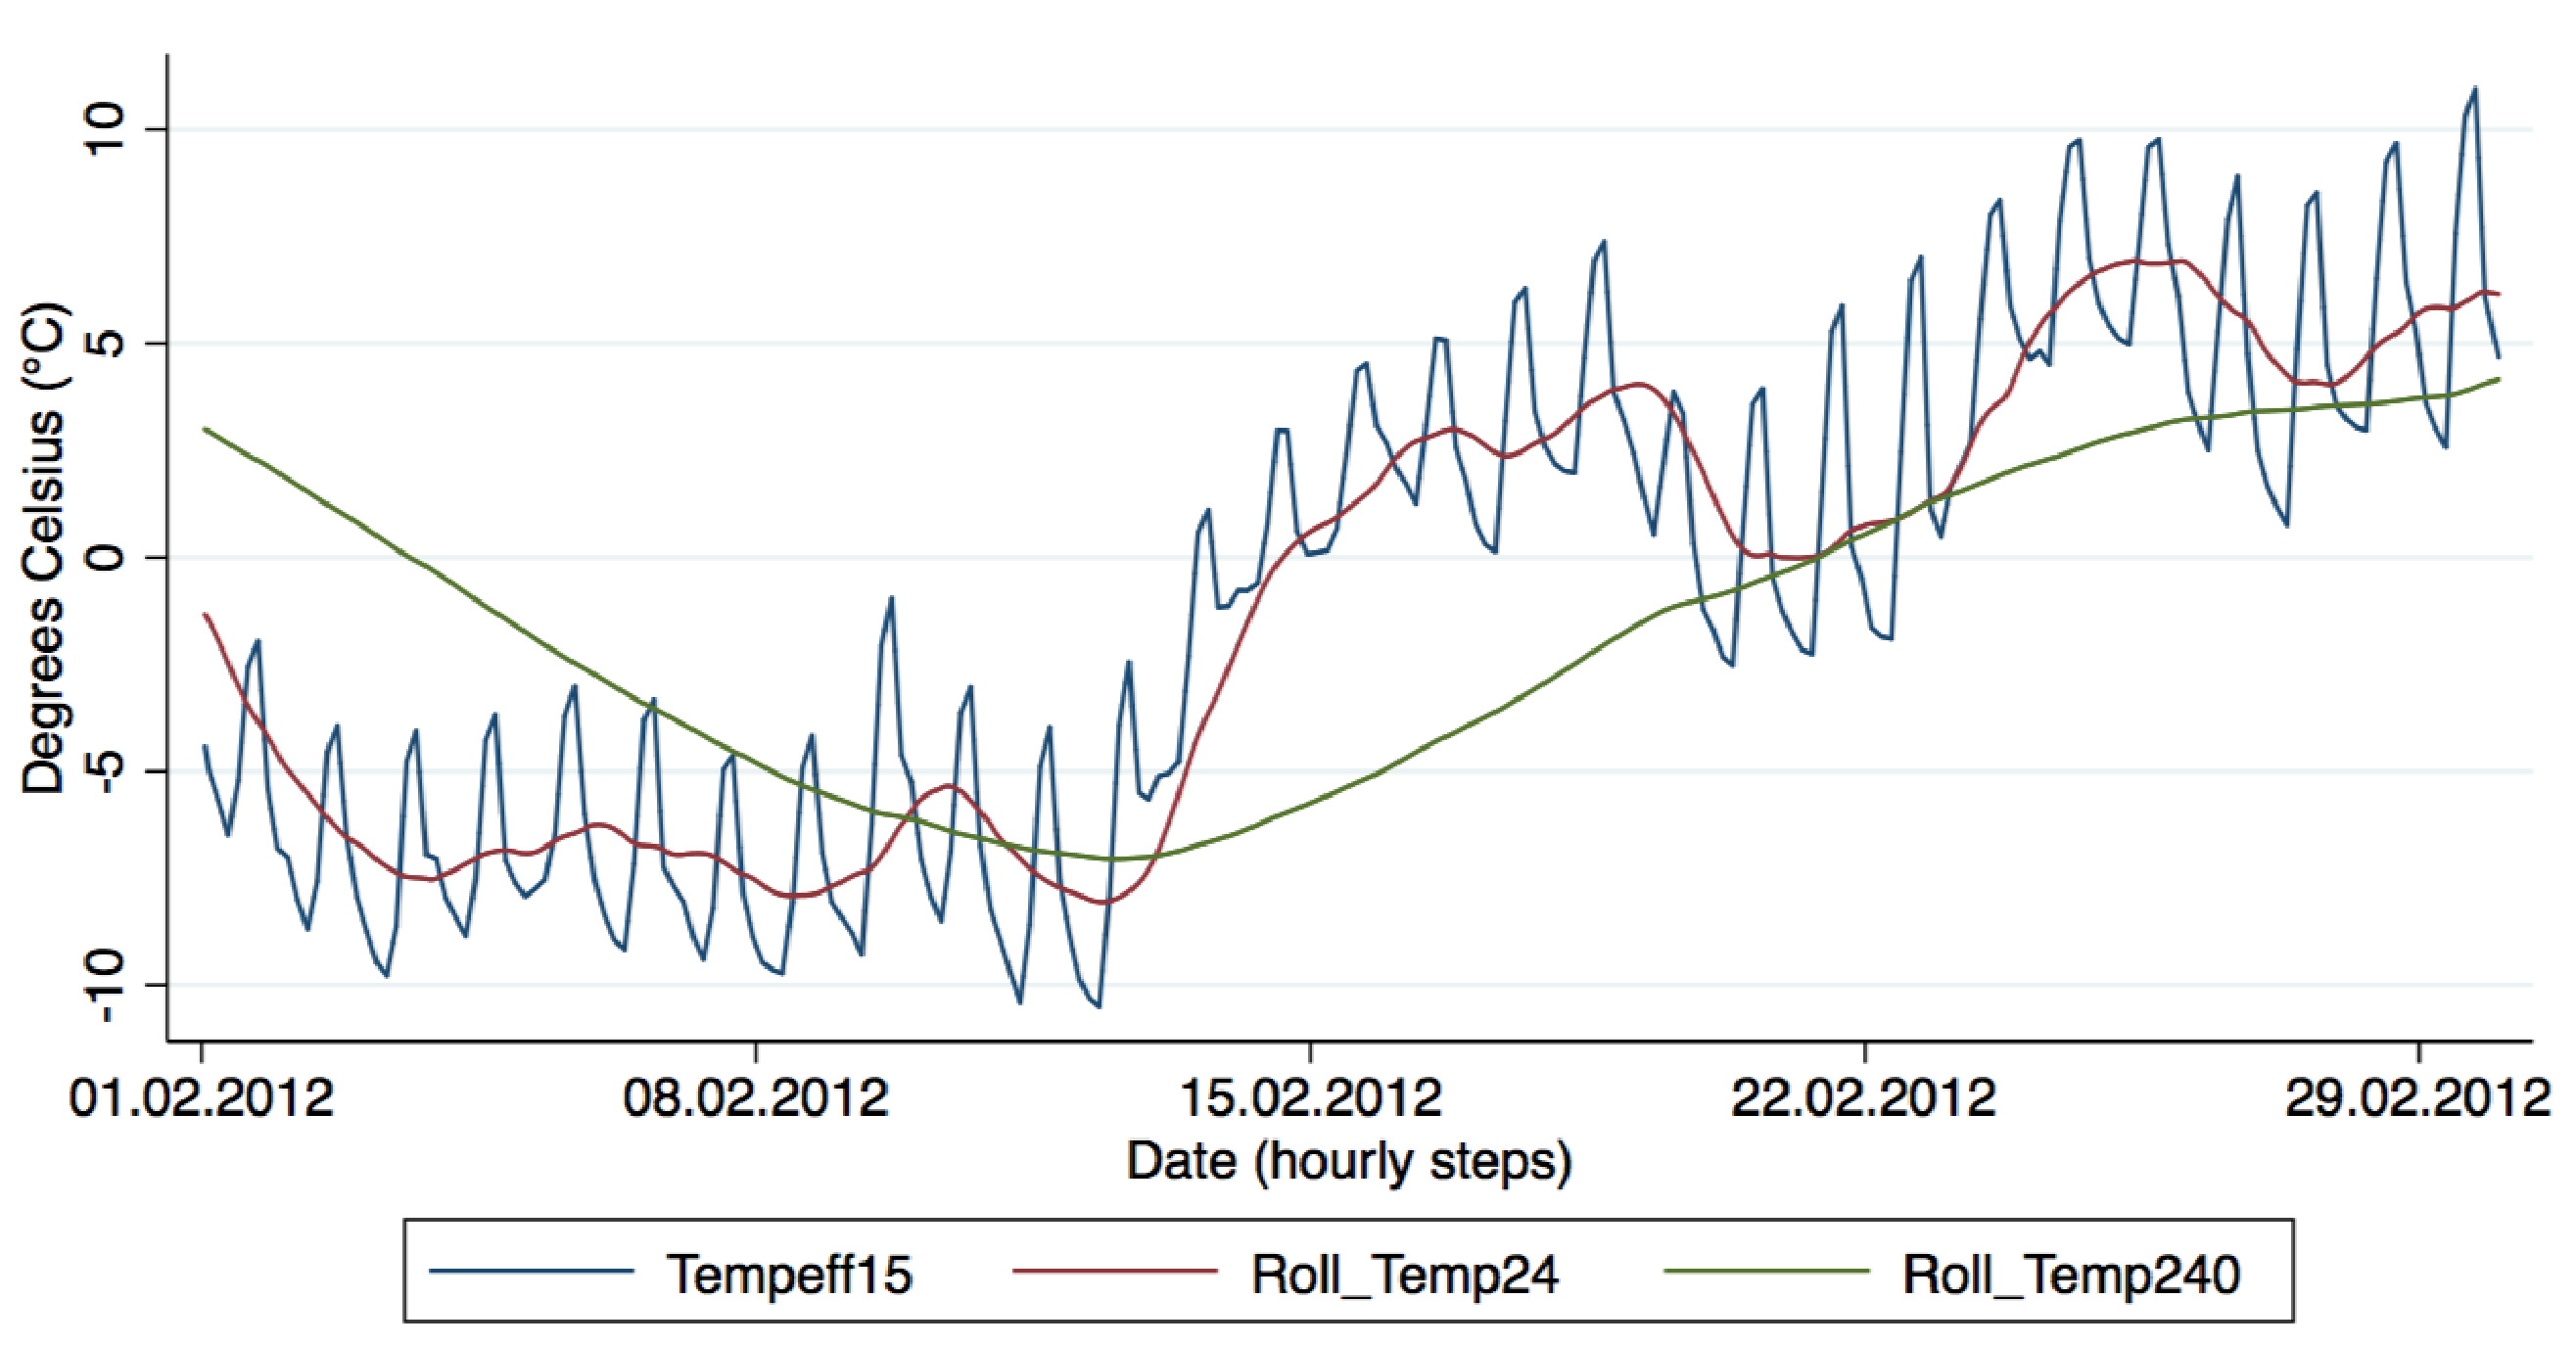
\includegraphics[height=50mm]{figch2/tempseasonality2.pdf} 
\caption{Temperature based seasonality controls}
\label{tempseasonality2}
\end{center}
\emph{Note: } The graph shows the evolution of the temperature based controls for seasonality for the month of February 2012. The graph shows the lagged nature of the rolling average temperature controls. 
\end{figure}
Fourth, we use the four variables suncycle, morning, deltasun and EWH collectively to continuously control for the time of the day. The reasoning is again the ability to get away from using dummies and being able to interpret the results. Figure \ref{seasonalityday3} shows how the controls describe the daily patterns continuously. \\

\begin{figure}[!ht]
\begin{center}
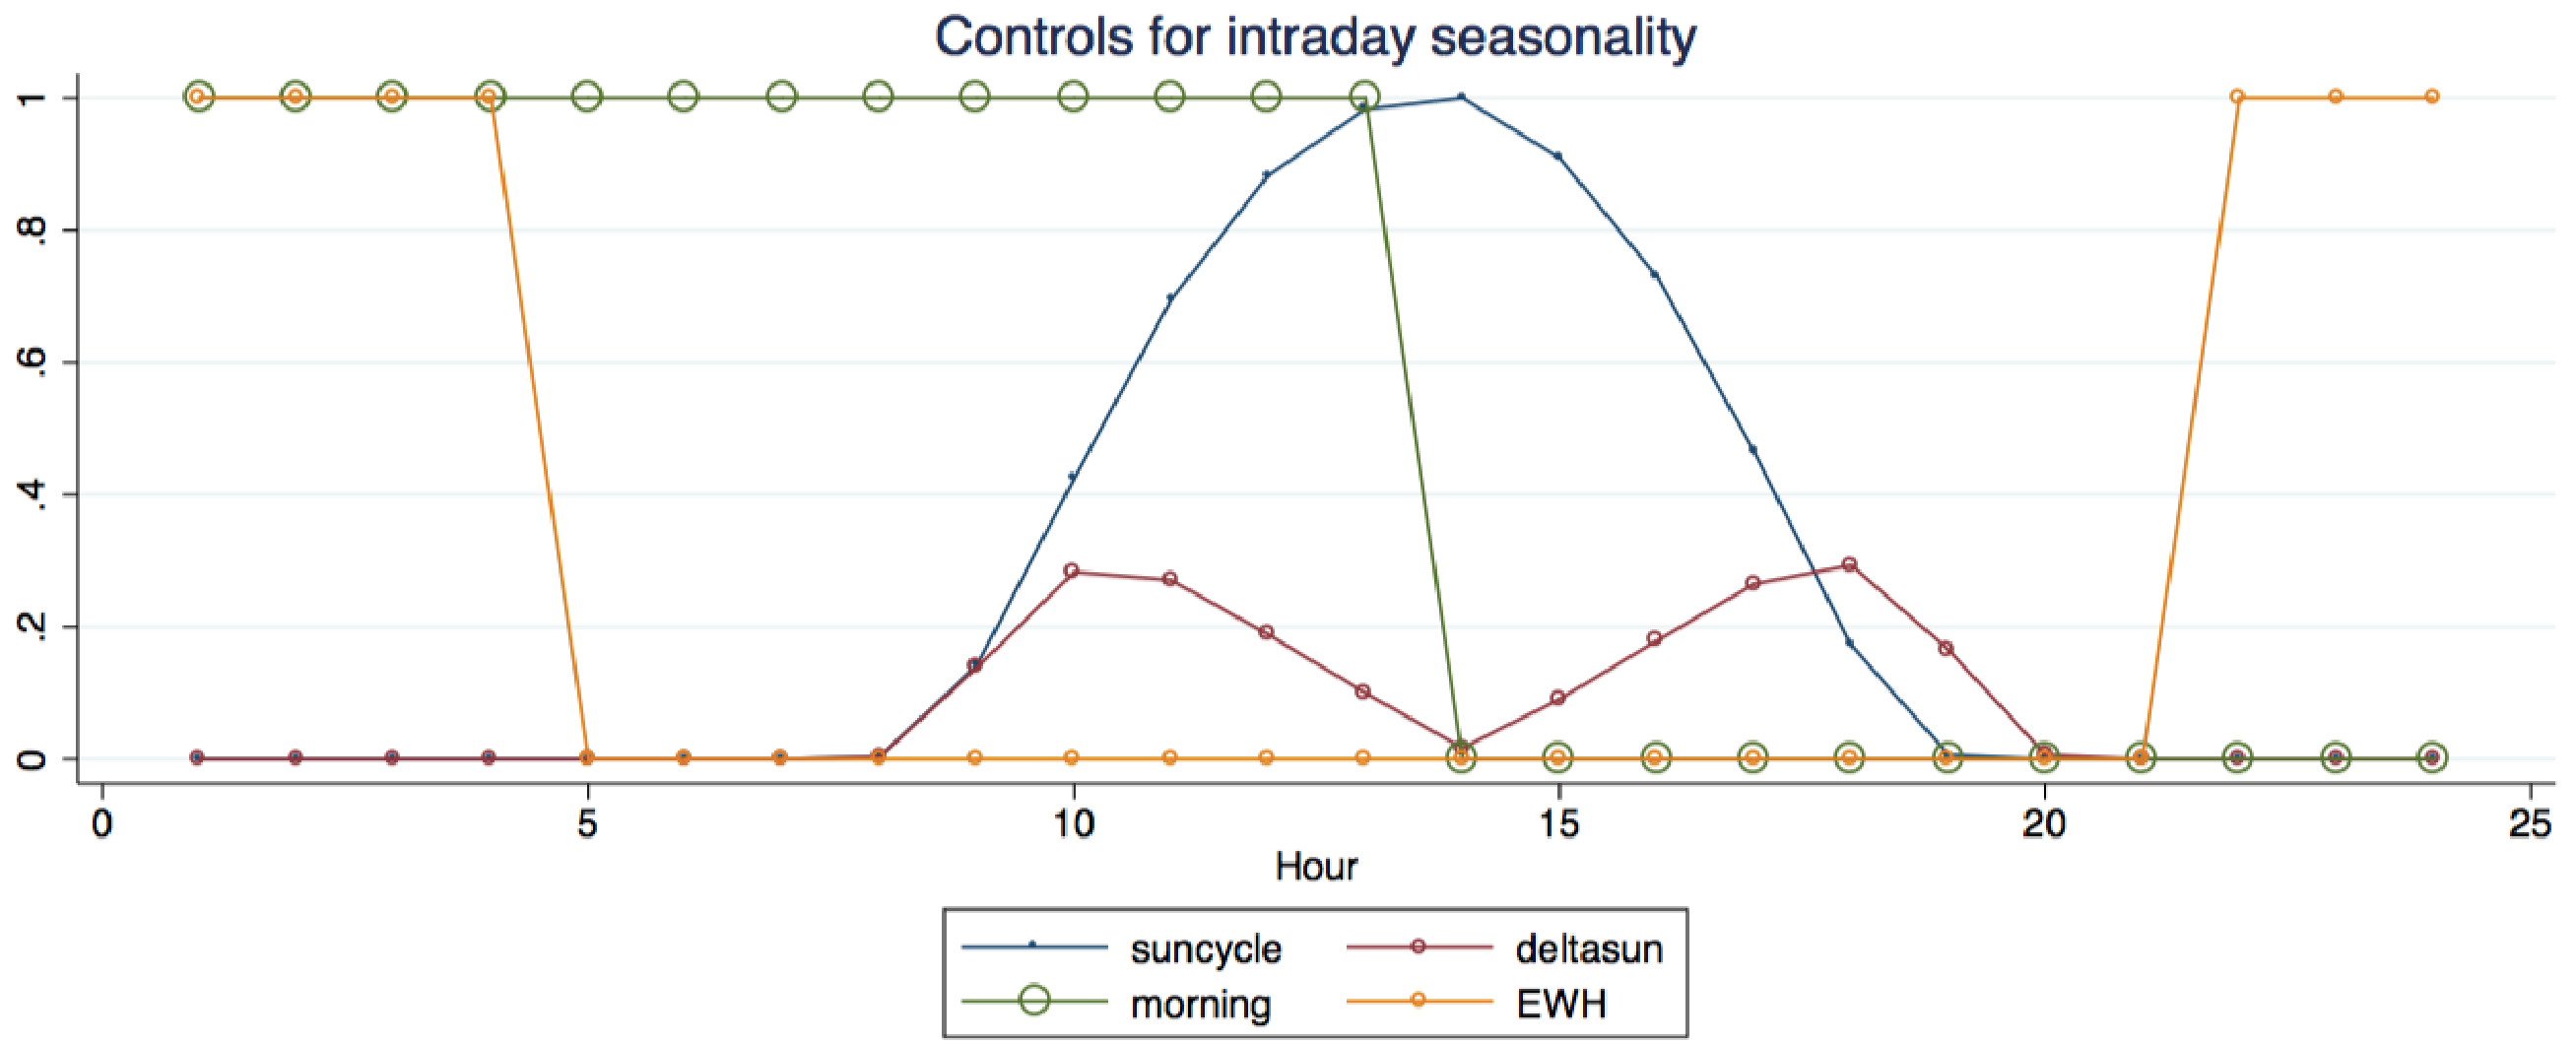
\includegraphics[height=50mm]{figch2/seasonalityday3.pdf} 
\caption{Continuous controls for daily patterns}
\label{seasonalityday3}
\end{center}
\emph{Note:} With the exception of EWH, all intraday seasonality controls (suncycle, morning, deltasun) are determined endogenously by the prevalent luminosity as captured by Solar.
\end{figure}
Fifth, SolarRest and RteBlackBox are the residual information gained from the variables Solar and the day ahead consumption prediction of RTE (PrevConsoH) over other variables included in $\boldsymbol{X^D}$ or $\boldsymbol{X^S}$, respectively.\footnote{E.g. Solar is strongly correlated with suncycle, thus SolarRest is the residual from a regression of the former on the latter. RteBlackBox is computed as the residuals from regressing PrevConsoH on Tempeff15,  Roll\_Temp24,  Roll\_Temp240, suncycle, morning, deltasun and EWH. See appendix \ref{SolarRest} and \ref{RteBlackBox} for details.}  \\
Sixth, Coal, Brent, Gas, IT2 and EUA are rough proxies for the input prices for electricity suppliers. Hydro is used as a crude proxy for dam operator's ability to generate short term electricity using hydro reserves. \\

We briefly emphasize that novel methodologies have been used to compute all variables derived from weather forecasts or observations. 
When tracing back the shape of aggregate bid functions on exogenous factors in the second stage estimation, we use aggregated statistics (at the national level) for the exogenous variables. We thus use an aggregation methodology to summarize local information (collected at the level of the individual postcodes) in order to generate an aggregate statistic at the national level. \\

The general methodology for the aggregation is explained using the example of Solar and as follows: We observe the value of a weather parameter (e.g. luminosity) every hour at known weather stations in France. 
We apply an interpolation technique in order to obtain parameter values for all possible geographic locations in France. At any local point, we can thus infer the electricity volume generated by using the information of the locally installed capacity (of solar panels) and the renewable energy available (i.e. sunlight inferred by the inverse of nebulosity). We then take the sum of all solar generated electricity per hour in France and use this as our aggregate statistic at the national level in our regression analyses. 
We used forecast data wherever possible in order to approximate the level of information that bidders have at the time of bidding and circumvent endogeneity problems. 
For cases where forecast data was not available, e.g. Solar, realised weather data was used. 


\subsubsection{Extensions and robustness checks}
In order to test the robustness of our results and circumvent some drawbacks of the baseline model, we use a few alternative specifications of our empirical model. 

\subsubsection{Bootstrapping standard errors}
The set-up of our empirical analysis relies on stochastic variables, e.g. PLU$^D$, which are computed in the first stage of our identification. The assumption made for an OLS regression of normally distributed residuals is a very strong one (particularly with the forecast variable) and one which can flaw the precision of estimates in the second stage regression. We therefore bootstrap the standard errors of the final regression by using random sampling with replacement at each stage of the analysis, i.e. for both the PLU computation and the final slope regression with 300 repetitions. \\

Bootstrapping allows us to non-parametrically approximate the distribution of the forecast PLUs and thus enables us to correct the standard errors of our coefficient estimates. 

\subparagraph{Kernel based uncertainty forecasts (PLU$^D$)}
\label{robustunc}

The PLU$^D$ computed as described in section \ref{proxyunc} is noisy since we assume a linear forecast model to be valid for any combination of realizations of exogenous paarameters, i.e. the same model applies winter and summer, day and night. While the results are as desired for the baseline PLU$^D$, a bootstrapping of the standard errors indicates that the first stage forecast is too imprecise for effects of a satisfactory significance level. \\

We therefore develop an extension of the uncertainty prediction model in which we use the idea of demand forecasts (equation \ref{predictu}) only locally, i.e. for a limited range of variation in the exogenous parameters. In other words, we estimate the PLU$^D$ corresponding to an auction only in the neighbourhood of this auction, i.e. over all auctions that occurred in similar conditions. By conditions, we mean realizations of exogenous parameters, and the neighbourhood refers to the concept of measuring the similarity of these realizations by means of a range. The next step explains how this is done formally. \\

We consider that firms predict the level of the uncertainty by comparing it with the level of uncertainty in past\footnote{For data availability reasons, we pool all (past and future) auctions for the computation of this PLU. This introduces some endogeneity. For a discussion of this choice, please see section \ref{endogeneityconcern}.} auctions of similar exogenous conditions. 
The methodology is analogous to the computation of the baseline PLU$^D$. The suppliers forecast the precision (squared residuals) of their demand estimation as before, but only on a subsample of the data. The subsample is defined as all observations which lie within a distance $b_{X_e}$ of the observation of interest with respect to each control variable~$X_e , \; \forall e=\{1,..,E\}$. Effectively, this is a multi-variate kernel regression and subsequent forecast with a rectangular (also called ``boxcar") weighting function. Observations within the kernel window are given equal weight, while observations outside the kernel window are given zero weight. We set the bandwidth $b_{X_e}$ with respect to each variable equal to $\frac{1}{3}$ of the range of that variable.\footnote{See appendix \ref{hardchoicePLU} for details. Column 2 of table \ref{multikernel} indicates the choice of $b_{X_e}$ for each exogenous variable considered.} \\

At any arbitrary observation (auction) with the realization $\boldsymbol{\tilde{X}}$ for the stacked vector of exogenous variables ($X_e$), the simple weight function is 
\begin{equation}
W(\boldsymbol{X}) =  \prod_{e} W(X_e) \; \text{,} \quad  \quad  \text{ where  } 
W(X_e) = \begin{cases} 1, \quad & \mbox{if } \vert \tilde{X_e} - X_e \vert \leq b_{X_e} 
%\quad  \forall X_e 
\\ 
0, \quad & \mbox{otherwise. } \end{cases}
\end{equation}
and the subsample based regressions are then
\begin{align}
P^D_k(\boldsymbol{X}) &= \alpha^{D,P}_{k,\boldsymbol{\tilde{X}}} + \beta^{D,P}_{k,\boldsymbol{\tilde{X}}} W(\boldsymbol{X}) + \epsilon^{D,P}_{k,\boldsymbol{\tilde{X}}} \\
Q^D_k(\boldsymbol{X}) &= \alpha^{D,Q}_{k,\boldsymbol{\tilde{X}}} + \beta^{D,Q}_{k,\boldsymbol{\tilde{X}}} W(\boldsymbol{X}) + \epsilon^{D,Q}_{k,\boldsymbol{\tilde{X}}} 
\end{align}
and the local uncertainty regressions and forecasts $\forall J=\{P,Q\} $ are given  by
\begin{align}
\bigl(\epsilon^{D,J}_{k,\boldsymbol{\tilde{X}}}\bigr)^2 &= \alpha^{U,J}_{k,\boldsymbol{\tilde{X}}} + \beta^{U,J}_{k,\boldsymbol{\tilde{X}}} W(\boldsymbol{X})  + \epsilon^{U,J}_{k,\boldsymbol{\tilde{X}}} \\
%
\underbrace{\widehat{\bigl(\epsilon^{D,J}_{k,\boldsymbol{\tilde{X}}}\bigr)}^2}_{\widehat{\text{PLU}}^D_{k, \boldsymbol{\tilde{X}}}} &= \alpha^{U,J}_{k,\boldsymbol{\tilde{X}}} + \beta^{U,J}_{k,\boldsymbol{\tilde{X}}} \boldsymbol{\tilde{X}}
\end{align}

When firms infer the upcoming uncertainty by looking at the uncertainty in past auctions, the precision of their estimate depends on the number of comparable auctions available, i.e. the sample size. Given that the sample size varies greatly across auctions, we use a sample-size-weighted OLS regression in the final estimation of equation \ref{secondstagereg2}. Finally, we bootstrap the standard errors on the kernel-based PLUs using 50 repetitions.\footnote{For computational reasons, we only bootstrap the kernel based PLUs for the point of inflection ($k=3$). We choose only 50 repetitions for the same reason. Given the size of our dataset, we consider it acceptable. The general criterion for convergence is that each observation is selected at least once in the bootstrapping exercise.}\\

\section{Results }
\label{resultsplusinterpret}
We first present the results for the demand estimation in both the Price and Volume dimension since this step is identical for all PLU specifications. We then present the results of the final regression in the baseline and alternative specifications. 

\subsection{Demand estimation}
Table \ref{VolDEPur52} gives the results for the demand estimation on volumes (equation \ref{regDQ}). Table \ref{PriceDEPur52} shows the results for the demand estimation on prices (equation \ref{regDP}). \\

These tables are interesting for two reasons. First, they provide the basis for our computation of the PLU$^D$. Second and the reason why we disclose them in such detail, they are already a result in themselves. \\

It is comforting to see that all variables used are significant and, more importantly, of the expected sign. This significance provides support for our specification of the demand estimation. For the interpretation here, we focus on the effects at the point of inflection\footnote{As mentioned, the point of inflection is the centre point of the bid curves and the most relevant for equilibrium determination. } ($k=3$). \\

First, looking at the volume effects of the exogenous variables: 
All variables included in the regression are highly significant at the $1\%$ level.
All temperature statistics (Tempeff15, Roll\_temp24, Roll\_temp240) bear coefficients with a negative sign and confirm that electricity demand falls with increasing ambient temperature. All daytime controls show up the expected sign as well: suncycle and deltasun have positive coefficients. This is sensible as electricity demand is higher during the day than at night (proxied for by suncycle) and rush or activity hours (proxied for by deltasun) in the morning and evening are also characterised by increased demand. The variables morning and EWH have coefficients of a plausible negative sign. The morning as controlled for by our indicator variable\footnote{The morning is defined as the hours before midday, which occurs when luminosity is at its daily maximum.} is shorter than the afternoon and evening together, thus total electricity consumption is lower as well. EWH stands for the deep night between 10 pm and 4 am and thus also corresponds to low demand periods. SolarRest controls for selfgeneration to cover own consumption and has a plausible negative coefficient. RteBlackBox, on the other hand, has a very sensible positive coefficient and confirms that actual demand is higher when the grid operator expects it to be the case. \\

The analysis of the price effects of these controls on demand functions is in line with the analysis of volume effects. This is coherent since for a linear downwards sloping demand curve, a left shift (volume decrease) is synonymous for a downwards shift (price decrease) of the curve. We consider that at the point $k=3$, the demand functions are locally linear. We note the only exception for the coefficient of SolarRest which has a positive price effect, while a negative volume effect.\footnote{We emphasize in the construction of our variable (appendix \ref{Solar}) that it is not possible to build a proxy for lighting consumption that would allow us to decorrelate the effects from photovoltaic production and lighting consumption. We therefore stick to the SolarRest proxy, which aims to capture the effect of Solar which is not captured by suncycle.} \\

Second, these tables already give a descriptive analysis of the effects of exogenous variables on the shape of the demand bid function:
We now compare all coefficients for a specific variable on the $K=5$ different points on the demand function (we read the table horizontally and compare sign changes across columns).\\

In table \ref{VolDEPur52}, we observe for each row at most a single sign change across the coefficients for the different points. Furthermore (and with few exceptions), the magnitudes of the coefficients generally increase or decrease monotonically along a row. 
This is very convincing as it suggests that exogenous variables have a monotone effect on the shape of the bid function. We thus only observe one-directional shifts (e.g. a unilateral left shift) or two-directional shifts (extension or contraction) in the volume dimension induced by the variation in exogenous variables. While the unilateral effects are explained analogously to our point specific interpretation on the point $k=3$ above, we do not have a story to tell about two-directional effects.\\

Tempeff15 results in a contraction of the bid function in terms of volumes (right shifts on low volume points, $k=5,4$ and left shifts on high volume points $k=3,2,1$). Roll\_Temp24 has the opposite effect and results in a volume extension of the curve. Roll\_Temp240 induces a pure left shift of the whole function.\footnote{Excluding interaction effects, we note that the net effect of a simultaneous 1$^o$C increase for all three temperature variables results in a net left shift of the function. In the price dimension (table \ref{PriceDEPur52}) we observe a net downwards shift. Both effects suggest that electricity demand decreases with the prevailing temperature.}
For the intraday seasonality controls, the results are very clear. While suncycle results in an extension of the demand function\footnote{Combined with the observed price effects from table \ref{PriceDEPur52}, this suggests that demand is more price elastic during the day.}, all other intraday controls (morning, deltasun, EWH) have unilateral effects. When the indicators morning and EWH are positive, we observe volume decreases at all points and thus a left shift of the function. Higher values of deltasun induces volume increases at all points of the bid function.\\

Finally, we have SolarRest which induces an expansion of the curve and RteBlackBox which has a unilateral right shifting effect on the aggregate demand bid function. \\

The price variation of the demand bid function yields interesting results, too. Given that the prices of points $k=1,5$ are fixed, we only observe effects for the interior points. We thus focus on the effects on the points $k=4,3,2$ only (called the ``central demand function" here). Again, we only observe at most a single sign change across columns for any exogenous variable. Both Tempeff15 and Roll\_Temp240 lead to an extension of the central demand function (we are now looking at vertical variation of the bid function as shown in fig. \ref{TypeallocK}), while Roll\_Temp24 causes a unilateral downwards shift. For intraday seasonality controls, we see that suncycle and deltasun have a contracting effect on the central demand function and morning a unilaterally negative effect. EWH leads to an expansion of the central demand function. 
SolarRest and RteBlackBox indicate an extension of the central demand function in the price dimension. \\

\newgeometry{margin=3cm} 
\begin{table}[!ht]
\vspace{2cm}
\begin{center}
\begin{center}
\begin{tabular}{lccccc} \toprule
% & (1) & (2) & (3) & (4) & (5) \\
&  $k=5$ & $k=4$ & $k=3$ & $k=2$ & $k=1$ \\
\textcolor{white}{VARIABLES} & Volume & Volume & Volume & Volume & Volume \\ \midrule
\vspace{4pt} & \begin{footnotesize}\end{footnotesize} & \begin{footnotesize}\end{footnotesize} & \begin{footnotesize}\end{footnotesize} & \begin{footnotesize}\end{footnotesize} & \begin{footnotesize}\end{footnotesize} \\
Tempeff15 & 50.72*** & 38.58*** & -130.3*** & -189.3*** & -204.0*** \\
\vspace{4pt} & \begin{footnotesize}(9.942)\end{footnotesize} & \begin{footnotesize}(10.13)\end{footnotesize} & \begin{footnotesize}(10.94)\end{footnotesize} & \begin{footnotesize}(13.32)\end{footnotesize} & \begin{footnotesize}(13.20)\end{footnotesize} \\
Roll\_Temp24 & -63.57*** & -67.13*** & -48.87*** & 19.76 & 34.16** \\
\vspace{4pt} & \begin{footnotesize}(11.78)\end{footnotesize} & \begin{footnotesize}(12.06)\end{footnotesize} & \begin{footnotesize}(13.14)\end{footnotesize} & \begin{footnotesize}(15.83)\end{footnotesize} & \begin{footnotesize}(15.76)\end{footnotesize} \\
Roll\_Temp240 & -60.15*** & -68.38*** & -78.49*** & -78.44*** & -87.38*** \\
\vspace{4pt} & \begin{footnotesize}(6.655)\end{footnotesize} & \begin{footnotesize}(6.867)\end{footnotesize} & \begin{footnotesize}(7.450)\end{footnotesize} & \begin{footnotesize}(10.05)\end{footnotesize} & \begin{footnotesize}(10.00)\end{footnotesize} \\
suncycle & -894.0*** & -652.1*** & 508.2*** & 1,351*** & 1,400*** \\
\vspace{4pt} & \begin{footnotesize}(44.27)\end{footnotesize} & \begin{footnotesize}(45.50)\end{footnotesize} & \begin{footnotesize}(48.52)\end{footnotesize} & \begin{footnotesize}(56.36)\end{footnotesize} & \begin{footnotesize}(55.73)\end{footnotesize} \\
morning & -101.2*** & -220.3*** & -814.8*** & -872.2*** & -885.8*** \\
\vspace{4pt} & \begin{footnotesize}(27.52)\end{footnotesize} & \begin{footnotesize}(28.33)\end{footnotesize} & \begin{footnotesize}(30.44)\end{footnotesize} & \begin{footnotesize}(37.71)\end{footnotesize} & \begin{footnotesize}(37.28)\end{footnotesize} \\
deltasun & 2,659*** & 2,850*** & 3,201*** & 1,721*** & 1,821*** \\
\vspace{4pt} & \begin{footnotesize}(153.5)\end{footnotesize} & \begin{footnotesize}(158.5)\end{footnotesize} & \begin{footnotesize}(166.1)\end{footnotesize} & \begin{footnotesize}(197.8)\end{footnotesize} & \begin{footnotesize}(196.5)\end{footnotesize} \\
EWH & -803.1*** & -833.1*** & -782.7*** & -354.7*** & -322.8*** \\
\vspace{4pt} & \begin{footnotesize}(30.74)\end{footnotesize} & \begin{footnotesize}(31.91)\end{footnotesize} & \begin{footnotesize}(33.15)\end{footnotesize} & \begin{footnotesize}(42.09)\end{footnotesize} & \begin{footnotesize}(41.78)\end{footnotesize} \\
SolarRest & -0.595*** & -0.363*** & -0.145*** & -0.0137 & 0.246*** \\
\vspace{4pt} & \begin{footnotesize}(0.0282)\end{footnotesize} & \begin{footnotesize}(0.0305)\end{footnotesize} & \begin{footnotesize}(0.0342)\end{footnotesize} & \begin{footnotesize}(0.0418)\end{footnotesize} & \begin{footnotesize}(0.0407)\end{footnotesize} \\
RteBlackBox & -0.00259 & 0.0127*** & 0.105*** & 0.107*** & 0.0979*** \\
\vspace{4pt} & \begin{footnotesize}(0.00235)\end{footnotesize} & \begin{footnotesize}(0.00243)\end{footnotesize} & \begin{footnotesize}(0.00255)\end{footnotesize} & \begin{footnotesize}(0.00316)\end{footnotesize} & \begin{footnotesize}(0.00317)\end{footnotesize} \\
Constant & 6,054*** & 7,086*** & 11,446*** & 15,215*** & 15,502*** \\
 & \begin{footnotesize}(33.71)\end{footnotesize} & \begin{footnotesize}(35.04)\end{footnotesize} & \begin{footnotesize}(37.15)\end{footnotesize} & \begin{footnotesize}(48.68)\end{footnotesize} & \begin{footnotesize}(48.27)\end{footnotesize} \\
\vspace{4pt} & \begin{footnotesize}\end{footnotesize} & \begin{footnotesize}\end{footnotesize} & \begin{footnotesize}\end{footnotesize} & \begin{footnotesize}\end{footnotesize} & \begin{footnotesize}\end{footnotesize} \\
\midrule Observations & 14,691 & 14,691 & 14,691 & 14,690 & 14,691 \\
$R^2$ & 0.201 & 0.219 & 0.478 & 0.344 & 0.346 \\
 White & 548.6 & 524.9 & 407.9 & 961.8 & 944.8 \\ \bottomrule
\multicolumn{6}{c}{\begin{footnotesize} Robust standard errors in parentheses\end{footnotesize}} \\
\multicolumn{6}{c}{\begin{footnotesize} *** p$<$0.01, ** p$<$0.05, * p$<$0.1\end{footnotesize}} \\
\end{tabular}
\end{center}

\caption{\label{VolDEPur52} Estimation results for demand volumes}
\end{center}
\emph{Note}: The estimated constants of this table or the left graph of fig. \ref{TypeallocK} indicate to which portion of the demand function the types of points $k=1,..,5$ refer. \\
\end{table}

\begin{table}[!ht]
\begin{center}
\begin{center}
\begin{tabular}{lccccc} \toprule
% & (1) & (2) & (3) & (4) & (5) \\
 & $k=5$ & $k=4$ & $k=3$ & $k=2$ & $k=1$\\
\textcolor{white}{VARIABLES} & Price & Price & Price & Price & Price \\ \midrule
\vspace{4pt} & \begin{footnotesize}\end{footnotesize} & \begin{footnotesize}\end{footnotesize} & \begin{footnotesize}\end{footnotesize} & \begin{footnotesize}\end{footnotesize} & \begin{footnotesize}\end{footnotesize} \\
Tempeff15 & 0 & 4.675*** & -0.969*** & -1.308*** & 0 \\
\vspace{4pt} & \begin{footnotesize}(0)\end{footnotesize} & \begin{footnotesize}(1.523)\end{footnotesize} & \begin{footnotesize}(0.0599)\end{footnotesize} & \begin{footnotesize}(0.0980)\end{footnotesize} & \begin{footnotesize}(0)\end{footnotesize} \\
Roll\_Temp24 & 0 & -10.07*** & -0.124* & -0.0470 & 0 \\
\vspace{4pt} & \begin{footnotesize}(0)\end{footnotesize} & \begin{footnotesize}(2.233)\end{footnotesize} & \begin{footnotesize}(0.0713)\end{footnotesize} & \begin{footnotesize}(0.116)\end{footnotesize} & \begin{footnotesize}(0)\end{footnotesize} \\
Roll\_Temp240 & 0 & 4.250*** & -0.0901** & -0.353*** & 0 \\
\vspace{4pt} & \begin{footnotesize}(0)\end{footnotesize} & \begin{footnotesize}(1.147)\end{footnotesize} & \begin{footnotesize}(0.0404)\end{footnotesize} & \begin{footnotesize}(0.0607)\end{footnotesize} & \begin{footnotesize}(0)\end{footnotesize} \\
suncycle & 0 & -10.98** & 6.870*** & 11.60*** & 0 \\
\vspace{4pt} & \begin{footnotesize}(0)\end{footnotesize} & \begin{footnotesize}(5.020)\end{footnotesize} & \begin{footnotesize}(0.258)\end{footnotesize} & \begin{footnotesize}(0.445)\end{footnotesize} & \begin{footnotesize}(0)\end{footnotesize} \\
morning & 0 & -0.226 & -5.748*** & -9.009*** & 0 \\
\vspace{4pt} & \begin{footnotesize}(0)\end{footnotesize} & \begin{footnotesize}(4.133)\end{footnotesize} & \begin{footnotesize}(0.173)\end{footnotesize} & \begin{footnotesize}(0.285)\end{footnotesize} & \begin{footnotesize}(0)\end{footnotesize} \\
deltasun & 0 & -16.54 & 10.60*** & 18.72*** & 0 \\
\vspace{4pt} & \begin{footnotesize}(0)\end{footnotesize} & \begin{footnotesize}(19.16)\end{footnotesize} & \begin{footnotesize}(0.881)\end{footnotesize} & \begin{footnotesize}(1.497)\end{footnotesize} & \begin{footnotesize}(0)\end{footnotesize} \\
EWH & 0 & 5.136 & -1.756*** & -3.014*** & 0 \\
\vspace{4pt} & \begin{footnotesize}(0)\end{footnotesize} & \begin{footnotesize}(4.448)\end{footnotesize} & \begin{footnotesize}(0.192)\end{footnotesize} & \begin{footnotesize}(0.302)\end{footnotesize} & \begin{footnotesize}(0)\end{footnotesize} \\
SolarRest & 0 & 0.000532 & 0.00192*** & 0.00253*** & 0 \\
\vspace{4pt} & \begin{footnotesize}(0)\end{footnotesize} & \begin{footnotesize}(0.00307)\end{footnotesize} & \begin{footnotesize}(0.000193)\end{footnotesize} & \begin{footnotesize}(0.000326)\end{footnotesize} & \begin{footnotesize}(0)\end{footnotesize} \\
RteBlackBox & 0 & 9.91e-05 & 0.000906*** & 0.00147*** & 0 \\
\vspace{4pt} & \begin{footnotesize}(0)\end{footnotesize} & \begin{footnotesize}(0.000301)\end{footnotesize} & \begin{footnotesize}(1.47e-05)\end{footnotesize} & \begin{footnotesize}(2.26e-05)\end{footnotesize} & \begin{footnotesize}(0)\end{footnotesize} \\
Constant & 3,000 & 131.3*** & 39.45*** & -39.43*** & -3,000 \\
 & \begin{footnotesize}(0)\end{footnotesize} & \begin{footnotesize}(4.210)\end{footnotesize} & \begin{footnotesize}(0.217)\end{footnotesize} & \begin{footnotesize}(0.319)\end{footnotesize} & \begin{footnotesize}(0)\end{footnotesize} \\
\vspace{4pt} & \begin{footnotesize}\end{footnotesize} & \begin{footnotesize}\end{footnotesize} & \begin{footnotesize}\end{footnotesize} & \begin{footnotesize}\end{footnotesize} & \begin{footnotesize}\end{footnotesize} \\
\midrule Observations & 14,691 & 14,691 & 14,691 & 14,690 & 14,691 \\
 $R^2$ &  & 0.005 & 0.463 & 0.420 &  \\ 
 White &  & 138.2 & 640.9 & 761.2 & \\ \bottomrule
\multicolumn{6}{c}{\begin{footnotesize} Robust standard errors in parentheses\end{footnotesize}} \\
\multicolumn{6}{c}{\begin{footnotesize} *** p$<$0.01, ** p$<$0.05, * p$<$0.1\end{footnotesize}} \\
\end{tabular}
\end{center}

\caption{\label{PriceDEPur52} Estimation results for demand prices }
\end{center}
\emph{Note}: The estimated constants of this table or the left graph of fig. \ref{TypeallocK} indicate to which portion of the demand function the types of points $k=1,..,5$ refer. \\
\end{table}
\restoregeometry


Overall, we take away a solid R$^2$ with coefficients of the correct sign. We furthermore have disclosed the White statistic which unanimously confirms heteroskedasticity in these regressions. The significance levels have been measured using robust standard errors. \\

We point to the fact that the explanatory power of our demand estimations is highest for the point of inflection, in line with our expectations. Points of maximum curvature $k=2,4$ reveal lower R$^2$ statistics. This is likely due to the underlying data patterns that arise from bidding frictions, e.g. focal price points. For these points, it is thus not surprising that we do not observe convincing demand estimates - we note in particular the lack of explanatory power for the demand estimation in the price dimension for points of type $k=4$. \\

\subsection{Final regression}
\label{discident}
For the final regression, we first lay the focus on the point of inflection ($k=3$) for a detailed interpretation of our results. We choose the point $k=3$, because this type of point is the most relevant for equilibrium determination. We then disclose the results for all other points $k \neq 3$ to give an overview of the effects of uncertainty on the whole aggregate supply bid function. \\

Each result table has four (three\footnote{For computational reasons, we do not run the bootstrapping of the kernel based PLU$^D$ for the points $k\neq 3$, thus we only have three columns for these tables.}) columns to show the results for different estimators and two specifications of the PLU$^D$. All other variables remain unchanged across the columns. In the tables, column 1 refers to the baseline specification of the PLU$^{D,J}$, where standard errors are calculated using the Huber-White sandwich estimator. Column 2 reports the results for the baseline model using bootstrapped standard errors with 300 repetitions. Column 3 reports the results for the regression on the kernel based PLU$^{D,J}_{\tilde{X}}$, using the sample size of each kernel as weights in the regression. Column 4 reports the results of the kernel based model using bootstrapped standard errors using 50 repetitions.\footnote{Coefficients vary slightly ($<\pm20\%$, no sign change), because the bootstrapping loop includes the kernel-based prediction of the uncertainty and thus varies the kernel sample sizes, which are used as weights in the final regression. Furthermore, the estimator has probably not yet fully converged with 50 repetitions, however for computational reasons we stick to this choice.} \\

\emph{Regarding notation:  } In the results tables, PLUvRvar`m' stands for PLU$^R_{1,m}$ with `m' being replaced by the initial of the variable in question (W, S and T, respectively). PLU$^R_{2,m}$ is indicated by the extension ``sq".  PLUvDvar`J' stands for PLU$^{D,J}$ with $J=\{P,Q\}$ representing the dimension in which the demand uncertainty is measured. The kernel based PLU$^D_{\tilde{X}}$ are given by PLUvDvarK`J' in the tables. To facilitate the reading of the tables, we adopt this notation for the discussion of the results. 


\paragraph{For the point of inflection ($k=3$),}
the results are shown in table \ref{main_1_5}. Regarding uncertainty from renewables production, only that of wind has a significant and robust impact. PLUvRvarW has a positive effect (significant at the 1\% level) on the slope in all specifications. PLUvRvarWsq has a negative effect on the slope in all specifications, however this second effect is not robust to bootstrapping the standard errors. The signs of the estimated coefficients are in line with our expectations. To show this, we recall that both versions of the PLUvRvarW are based on the inverse of the characteristic lengthscale $L_W$ of autocorrelation of the wind speed measurements. Thus, when $L_W$ increases (it represents a decrease in the uncertainty since wind speeds are homogenous over longer distances), the PLU decreases (corresponding to a decrease in uncertainty). \\

While an increase in the PLUvRvarW leads to an increase in the slope of the supply function, the effect is attenuated by the squared term PLUvRvarWsq for very small and large $L_W$.\footnote{By looking at the variation of our data, we see that the negative effect of the PLUvRvarWsq term merely attenuates, rather than overrides, the positive effect of the PLUvRvarW term on the slope since in our dataset we very rarely observe PLUvRvarW values sufficiently large to exceed the maximum of the Laffer curve of the impact on the slope.} The estimated coefficient for the latter is negative and suggests that for very short $L_W$ (i.e. very heterogenous wind speeds over the country), prediction errors cancel out. For very long $L_W$ (i.e. very homogenous wind speed profile), the marginal impact of $L_W$ on the level of uncertainty decreases. \\

With respect to the uncertainty from temperature forecasts, the results are insignificant (although of the anticipated sign). We expect the impact of temperature uncertainty goes via the demand response, which we account for in our proxy for the uncertainty from demand realization (PLUvD). Similarly, uncertainty from Solar production is attributed no effect. This is not surprising as generation from solar is only a fraction of that generated from wind power and thus negligible. Furthermore, we are unable to disentangle the effect of solar generation from the reduced demand effect from high luminosity (which result in low demand for lighting). We do not find evidence for a direct response from suppliers to uncertainty in temperature or solar predictions. \\

Uncertainty from the realization of market demand has a negative and significant effect when proxied for by price-based PLUvDvarP (see table \ref{main_1_5}) as opposed to a positive and significant effect when proxied for by a volume-based PLUvDvarQ (see table \ref{main_1_5}). 
The positive effect on PLUvDvarQ is in line with our prediction made in section \ref{intropredict}. This result supports the theory that firms take uncertainty when bidding into account and consequently adjust their bidding strategy in order to minimize dynamic costs. \\

However, our theory produces a prediction for volume based uncertainty only. We include the uncertainty proxy for price PLUvDvarP as a control and its effect seems rather robust. The effects of PLUvD in either the price or volume dimension are robust to the exclusion of the other.\footnote{Results available from the authors.} We try to explain the opposing signs for the coefficients of the two proxies in section \ref{findings}.\footnote{The net effect cannot be precisely computed as the conversion of the PLUvD from the price dimension to the quantity dimension is not possible. We approximate the comparison however, by including both PLU$^{D}$ simultaneously in the regression. All PLUvD are rescaled by their respective means to allow some degree of comparison.} \\

Furthermore, table \ref{main_1_5} gives support to our extension using kernel based PLUvDs. Column~2 shows that the effects of the baseline PLUvD are not significant when bootstrapped. Our alternative is to use a more elaborate uncertainty prediction model.  These kernel based PLUvD are more sophisticated in two respects: (i) the forecasting model is only applied locally, that is auctions are only compared to similar auctions and (ii) the obtained forecast is weighted by the sample size used for its prediction. Thereby, we control for the confidence of the firms in making those predictions. The results of the weighted regression are given in column 3. The results using the more elaborate prediction model are in line with those from the baseline regression, while being more accurate as indicated by the improved explanatory power of our model (we see a $16.5\%$ increase of the R$^2$ from columns 1-2 to columns 3-4). Finally, the results of our kernel based model are more precise as indicated by the higher significance level for the PLUvDvarKP and PLUvDvarKQ, which are now also robust to a bootstrap (column~4).\\

Finally, we explicitly include the controls for the levels of the input prices of electricity producers ($\boldsymbol{X^S}$). We do not interpret these coefficients since there are no ex-ante expectations of their levels to affect the slope of the supply bid function. We briefly mention that intraday seasonality controls as well as other demand related variables are not included in this regression to avoid multicollinearity problems with the PLUvD, which are themselves computed as a linear combination of the demand control variables~($\boldsymbol{X^D}$). \\

Overall, we take away a goodness of fit of $\geq 20\%$ for our empirical model as well as the robust positive coefficients for both the demand based uncertainty proxy (PLUvDvarQ) and the weather based uncertainty proxies (PLUvRvarW and PLUvRvarWsq). We note the puzzling result for the PLUvDvarP. 

\begin{table}[!ht]
\vspace{-2.38cm}
\begin{center}
\begin{tabular}{lcccc}
\multicolumn{5}{c}{\begin{large}For k=3 (Point of inflection)\end{large}} \\ \midrule
 & (1) & (2) & (3) & (4) \\
% & d1short1\_5 & bs\_baseline\_5 & kernel4\_5 & kernel5\_5 \\
\textcolor{white}{VARIABLES} & fxInvertQP & fxInvertQP & fxInvertQP & fxInvertQP \\ \midrule
\vspace{4pt} & \begin{footnotesize}\end{footnotesize} & \begin{footnotesize}\end{footnotesize} & \begin{footnotesize}\end{footnotesize} & \begin{footnotesize}\end{footnotesize} \\
PLUvRvarT & 0.000882 & 0.000882 & 0.00374** & 0.00508 \\
\vspace{4pt} & \begin{footnotesize}(0.00152)\end{footnotesize} & \begin{footnotesize}(0.00415)\end{footnotesize} & \begin{footnotesize}(0.00155)\end{footnotesize} & \begin{footnotesize}(0.00354)\end{footnotesize} \\
PLUvRvarTsq & -0.000529 & -0.000529 & -0.00161*** & -0.00215 \\
\vspace{4pt} & \begin{footnotesize}(0.000584)\end{footnotesize} & \begin{footnotesize}(0.168)\end{footnotesize} & \begin{footnotesize}(0.000603)\end{footnotesize} & \begin{footnotesize}(0.183)\end{footnotesize} \\
PLUvRvarW & 0.00790*** & 0.00790*** & 0.00647*** & 0.00574*** \\
\vspace{4pt} & \begin{footnotesize}(0.00123)\end{footnotesize} & \begin{footnotesize}(0.00257)\end{footnotesize} & \begin{footnotesize}(0.00121)\end{footnotesize} & \begin{footnotesize}(0.00207)\end{footnotesize} \\
PLUvRvarWsq & -0.00235*** & -0.00235 & -0.00192*** & -0.00170 \\
\vspace{4pt} & \begin{footnotesize}(0.000373)\end{footnotesize} & \begin{footnotesize}(0.0644)\end{footnotesize} & \begin{footnotesize}(0.000370)\end{footnotesize} & \begin{footnotesize}(0.0479)\end{footnotesize} \\
PLUvRvarS & -5.20e-10 & -5.20e-10 & -2.28e-09 & -2.23e-09 \\
\vspace{4pt} & \begin{footnotesize}(2.68e-09)\end{footnotesize} & \begin{footnotesize}(3.58e-08)\end{footnotesize} & \begin{footnotesize}(3.16e-09)\end{footnotesize} & \begin{footnotesize}(3.69e-08)\end{footnotesize} \\
PLUvRvarSsq & 0 & 0 & 0 & 0 \\
\vspace{4pt} & \begin{footnotesize}(0)\end{footnotesize} & \begin{footnotesize}(0)\end{footnotesize} & \begin{footnotesize}(0)\end{footnotesize} & \begin{footnotesize}(0)\end{footnotesize} \\
Coal & 6.90e-06*** & 6.90e-06*** & 5.18e-06*** & 6.29e-06*** \\
\vspace{4pt} & \begin{footnotesize}(4.35e-07)\end{footnotesize} & \begin{footnotesize}(4.64e-07)\end{footnotesize} & \begin{footnotesize}(4.39e-07)\end{footnotesize} & \begin{footnotesize}(6.87e-07)\end{footnotesize} \\
Brent & -2.36e-05*** & -2.36e-05*** & -1.18e-05*** & -1.40e-05*** \\
\vspace{4pt} & \begin{footnotesize}(1.51e-06)\end{footnotesize} & \begin{footnotesize}(1.96e-06)\end{footnotesize} & \begin{footnotesize}(1.53e-06)\end{footnotesize} & \begin{footnotesize}(2.01e-06)\end{footnotesize} \\
Gas & -2.82e-07 & -2.82e-07 & 1.37e-05*** & 1.36e-05*** \\
\vspace{4pt} & \begin{footnotesize}(1.89e-06)\end{footnotesize} & \begin{footnotesize}(9.41e-06)\end{footnotesize} & \begin{footnotesize}(1.67e-06)\end{footnotesize} & \begin{footnotesize}(2.46e-06)\end{footnotesize} \\
IT2 & -2.71e-05*** & -2.71e-05 & -1.73e-05*** & -1.99e-05*** \\
\vspace{4pt} & \begin{footnotesize}(2.17e-06)\end{footnotesize} & \begin{footnotesize}(1.80e-05)\end{footnotesize} & \begin{footnotesize}(1.34e-06)\end{footnotesize} & \begin{footnotesize}(1.69e-06)\end{footnotesize} \\
EUA & 7.20e-05*** & 7.20e-05*** & 2.62e-05*** & 2.71e-05*** \\
\vspace{4pt} & \begin{footnotesize}(2.31e-06)\end{footnotesize} & \begin{footnotesize}(4.49e-06)\end{footnotesize} & \begin{footnotesize}(3.34e-06)\end{footnotesize} & \begin{footnotesize}(6.84e-06)\end{footnotesize} \\
Wind1DA & 1.04e-07*** & 1.04e-07*** & 1.18e-07*** & 1.25e-07*** \\
\vspace{4pt} & \begin{footnotesize}(6.45e-09)\end{footnotesize} & \begin{footnotesize}(1.03e-08)\end{footnotesize} & \begin{footnotesize}(6.51e-09)\end{footnotesize} & \begin{footnotesize}(7.63e-09)\end{footnotesize} \\
Hydro & -7.55e-06*** & -7.55e-06*** & -4.08e-06*** & -5.88e-06*** \\
\vspace{4pt} & \begin{footnotesize}(8.33e-07)\end{footnotesize} & \begin{footnotesize}(2.24e-06)\end{footnotesize} & \begin{footnotesize}(8.61e-07)\end{footnotesize} & \begin{footnotesize}(1.11e-06)\end{footnotesize} \\
PLUvDvarP & -0.000219*** & -0.000219 &  &  \\
\vspace{4pt} & \begin{footnotesize}(4.57e-05)\end{footnotesize} & \begin{footnotesize}(0.000203)\end{footnotesize} & \begin{footnotesize}\end{footnotesize} & \begin{footnotesize}\end{footnotesize} \\
PLUvDvarQ & 0.000567*** & 0.000567 &  &  \\
\vspace{4pt} & \begin{footnotesize}(9.44e-05)\end{footnotesize} & \begin{footnotesize}(0.000585)\end{footnotesize} & \begin{footnotesize}\end{footnotesize} & \begin{footnotesize}\end{footnotesize} \\
PLUvDvarKP &  &  & -0.000600*** & -0.000462*** \\
\vspace{4pt} & \begin{footnotesize}\end{footnotesize} & \begin{footnotesize}\end{footnotesize} & \begin{footnotesize}(2.69e-05)\end{footnotesize} & \begin{footnotesize}(4.24e-05)\end{footnotesize} \\
PLUvDvarKQ &  &  & 0.000151*** & 0.000170** \\
\vspace{4pt} & \begin{footnotesize}\end{footnotesize} & \begin{footnotesize}\end{footnotesize} & \begin{footnotesize}(3.39e-05)\end{footnotesize} & \begin{footnotesize}(6.80e-05)\end{footnotesize} \\
Constant & 0.00651*** & 0.00651*** & 0.00513*** & 0.00538*** \\
 & \begin{footnotesize}(0.000208)\end{footnotesize} & \begin{footnotesize}(0.000789)\end{footnotesize} & \begin{footnotesize}(0.000195)\end{footnotesize} & \begin{footnotesize}(0.000257)\end{footnotesize} \\
%\vspace{4pt} & \begin{footnotesize}\end{footnotesize} & \begin{footnotesize}\end{footnotesize} & \begin{footnotesize}\end{footnotesize} & \begin{footnotesize}\end{footnotesize} \\
\midrule Observations & 11,702 & 11,702 & 11,702 & 11,702 \\
 $R^2$ & 0.200 & 0.200 & 0.233 & 0.234 \\ \bottomrule
\multicolumn{5}{c}{\begin{footnotesize} (Standard errors in parentheses)\end{footnotesize}} \\
\multicolumn{5}{c}{\begin{footnotesize} *** p$<$0.01, ** p$<$0.05, * p$<$0.1\end{footnotesize}} \\
\end{tabular}
\end{center}

\caption{\label{main_1_5} Regressions of the slope on PLU$^R$ and PLU$^{D}$ and PLU$^{D}$ at $k=3$}
\emph{Note}: Standard errors are reported in parenthesis. Column 1 refers to the baseline specification. Column 2 reports bootstrapped results for the baseline model. Column 3 reports the results for the (weighted) regression on the kernel based PLU$^D_{\tilde{X}}$. Column 4 reports bootstrapped results of the model in column 3. 
\end{table}
\pagestyle{empty}

\section*{}
\paragraph{For the other points  ($k=1,2,4,5$),} the results are given in tables \ref{mainNS1_1}, \ref{mainNS1_3}, \ref{mainNS1_7} and \ref{mainNS1_9}, respectively.\footnote{Variables marked ``(omitted)" are drop due to perfect collinearity.} We comment on the effects over all points collectively in order to give an overview of the full bid function behaviour.\\

The specification of the proxies for the uncertainty from renewables as well as of the controls does not vary across columns, we thus focus on column 2 for these (in order to take bootstrapped standard errors into account). 
While we observe in table \ref{main_1_5} a convincing effect for the uncertainty from wind predictions on the slope of the point of inflection ($k=3$), we cannot observe this effects on the other points of the bid function.\footnote{We note the exception of a negative effect for PLUvRvarW on the slopes at points $k=2$ and 5 (significant at the $5\%$ level).} No other proxy for the uncertainty from renewables has a significant effect on the slope at any point. \\

The proxies for uncertainty from market demand produce opposing effect depending on the prediction model. PLUvDvarP has a negative and significant effect on all points (with the exception of points $k=1$ and $k=5$ of course, which do not exhibit variation in prices due to the auction rules). PLUvDvarQ has a positive effect, when significant\footnote{For both the bootstrapped baseline results (col. 2) and the weighted kernel based specification (col. 3). }, on all points ($k=2-5$), but not on $k=1$. \\

On the remaining controls, we do not observe a clear pattern on the effects at the different points. We run the analysis without these controls and note that the signs of all significant variables remain unchanged.\footnote{Results available from the authors.}\\

\begin{table}[!ht]
\vspace{-2.5cm}
\begin{center}
\begin{tabular}{lccc}
\multicolumn{4}{c}{\begin{large}For k=1 (Left extremal point) \end{large}} \\ \midrule
 & (1) & (2) & (3) \\
% & d1short1\_1 & bs\_baseline\_1 & kernel4\_1 \\
\textcolor{white}{VARIABLES} & fxInvertQP & fxInvertQP & fxInvertQP \\ \midrule
\vspace{4pt} & \begin{footnotesize}\end{footnotesize} & \begin{footnotesize}\end{footnotesize} & \begin{footnotesize}\end{footnotesize} \\
PLUvRvarT & -4.14e-05*** & -4.14e-05 & 0.000277* \\
PLUvRvarTsq & 1.56e-05*** & 1.56e-05 & -0.0122 \\
PLUvRvarW & -6.04e-06 & -6.04e-06 & -0.000138 \\
PLUvRvarWsq & 1.71e-06 & 1.71e-06 & 0.00738 \\
PLUvRvarS & 0 & 0 & -5.70e-05 \\
PLUvRvarSsq & -0 & -0 & 0.00172 \\
Coal & -8.54e-09*** & -8.54e-09*** & (omitted) \\
Brent & 8.64e-08*** & 8.64e-08*** & (omitted) \\
Gas & -6.20e-08*** & -6.20e-08*** & (omitted) \\
IT2 & 4.95e-08*** & 4.95e-08*** & 3.50e-08 \\
EUA & -3.14e-08*** & -3.14e-08*** & 4.43e-06*** \\
Wind1DA & -3.38e-10*** & -3.38e-10*** & 2.48e-10 \\
Hydro & 4.69e-08*** & 4.69e-08*** & (omitted) \\
PLUvDvarQ & -3.87e-06*** & -3.87e-06*** &  \\
PLUvDvarKQ &  &  & -7.21e-10*** \\
Constant & 2.11e-06*** & 2.11e-06** & -6.00e-05*** \\
%\vspace{4pt} & \begin{footnotesize}\end{footnotesize} & \begin{footnotesize}\end{footnotesize} & \begin{footnotesize}\end{footnotesize} \\
\midrule Observations & 11,702 & 11,702 & 50 \\
 $R^2$ & 0.152 & 0.152 & 0.681 \\ \bottomrule
\multicolumn{4}{c}{\begin{footnotesize} Standard errors available from the authors\end{footnotesize}} \\
\multicolumn{4}{c}{\begin{footnotesize} *** p$<$0.01, ** p$<$0.05, * p$<$0.1\end{footnotesize}} \\
\end{tabular}
\end{center}

\vspace{-0.2cm}
\caption{\label{mainNS1_1} Regressions of slope on PLU$^R$ and PLU$^{D}$ and PLU$^{D}$ at $k=1$}
\vspace{0.9cm}
\begin{center}
\begin{tabular}{lccc}
\multicolumn{4}{c}{\begin{large}For k=2 (Left point of maximum curvature)\end{large}} \\ \midrule
 & (1) & (2) & (3) \\
% & d1short1\_3 & bs\_baseline\_3 & kernel4\_3 \\
\textcolor{white}{VARIABLES} & fxInvertQP & fxInvertQP & fxInvertQP \\ \midrule
\vspace{4pt} & \begin{footnotesize}\end{footnotesize} & \begin{footnotesize}\end{footnotesize} & \begin{footnotesize}\end{footnotesize} \\
PLUvRvarT & -0.00252 & -0.00252 & 0.292 \\
PLUvRvarTsq & 0.00106 & 0.00106 & -17.27 \\
PLUvRvarW & -0.00549*** & -0.00549** & 0.339 \\
PLUvRvarWsq & 0.00158*** & 0.00158 & -21.86 \\
PLUvRvarS & -6.82e-10 & -6.82e-10 & 0.0669 \\
PLUvRvarSsq & 0 & 0 & -1.968 \\
Coal & 2.36e-06*** & 2.36e-06*** & (omitted) \\
Brent & -1.86e-05*** & -1.86e-05*** & (omitted)  \\
Gas & -8.94e-06*** & -8.94e-06*** & (omitted) \\
IT2 & 1.98e-05*** & 1.98e-05*** & 6.92e-05 \\
EUA & 8.69e-05*** & 8.69e-05*** & -0.000439 \\
Wind1DA & 6.13e-09 & 6.13e-09 & 6.70e-07 \\
Hydro & -5.82e-06*** & -5.82e-06*** & (omitted) \\
PLUvDvarP & -4.81e-05*** & -4.81e-05*** &  \\
PLUvDvarQ & 0.000442*** & 0.000442*** &  \\
PLUvDvarKP &  &  & -9.62e-07* \\
PLUvDvarKQ &  &  & -4.27e-07 \\
Constant & 0.00319*** & 0.00319*** & 0.00279 \\
%\vspace{4pt} & \begin{footnotesize}\end{footnotesize} & \begin{footnotesize}\end{footnotesize} & \begin{footnotesize}\end{footnotesize} \\
\midrule Observations & 11,702 & 11,702 & 50 \\
 $R^2$ & 0.158 & 0.158 & 0.414 \\ \bottomrule
\multicolumn{4}{c}{\begin{footnotesize} Standard errors available from the authors\end{footnotesize}} \\
\multicolumn{4}{c}{\begin{footnotesize} *** p$<$0.01, ** p$<$0.05, * p$<$0.1\end{footnotesize}} \\
\end{tabular}
\end{center}

\vspace{-0.2cm}
\caption{\label{mainNS1_3} Regressions of slope on PLU$^R$ and PLU$^{D}$ and PLU$^{D}$ at $k=2$}
\end{table}
\pagestyle{empty}

\begin{table}[!ht]
\vspace{-2.5cm}
\begin{center}
\begin{tabular}{lccc}
\multicolumn{4}{c}{\begin{large}For k=4 (Right point of maximum curvature)\end{large}} \\ \midrule
 & (1) & (2) & (3) \\
% & d1short1\_7 & bs\_baseline\_7 & kernel4\_7 \\
\textcolor{white}{VARIABLES} & fxInvertQP & fxInvertQP & fxInvertQP \\ \midrule
\vspace{4pt} & \begin{footnotesize}\end{footnotesize} & \begin{footnotesize}\end{footnotesize} & \begin{footnotesize}\end{footnotesize} \\
PLUvRvarT & -0.00442*** & -0.00442 & 0.000559 \\
PLUvRvarTsq & 0.00149** & 0.00149 & -0.000368 \\
PLUvRvarW & -0.000137 & -0.000137 & -0.00205 \\
PLUvRvarWsq & 0.000173 & 0.000173 & 0.000739* \\
PLUvRvarS & 2.59e-09 & 2.59e-09 & 2.40e-09 \\
PLUvRvarSsq & -0 & -0 & -0 \\
Coal & 2.22e-07 & 2.22e-07 & 1.48e-06*** \\
Brent & -7.46e-06*** & -7.46e-06*** & -1.30e-05*** \\
Gas & 9.04e-06*** & 9.04e-06*** & 2.04e-05*** \\
IT2 & -1.96e-05*** & -1.96e-05*** & -2.61e-05*** \\
EUA & 4.71e-05*** & 4.71e-05*** & 3.19e-05*** \\
Wind1DA & 1.64e-08** & 1.64e-08** & 1.50e-08** \\
Hydro & -8.73e-06*** & -8.73e-06*** & -1.33e-05*** \\
PLUvDvarP & -0.000212*** & -0.000212*** &  \\
PLUvDvarQ & 0.000110 & 0.000110** &  \\
PLUvDvarKP &  &  & -0.000163*** \\
PLUvDvarKQ &  &  & 4.08e-05 \\
Constant & 0.00370*** & 0.00370*** & 0.00406*** \\
%\vspace{4pt} & \begin{footnotesize}\end{footnotesize} & \begin{footnotesize}\end{footnotesize} & \begin{footnotesize}\end{footnotesize} \\
\midrule Observations & 11,701 & 11,701 & 11,701 \\
 $R^2$ & 0.086 & 0.086 & 0.117 \\ \bottomrule
\multicolumn{4}{c}{\begin{footnotesize} Standard errors available from the authors\end{footnotesize}} \\
\multicolumn{4}{c}{\begin{footnotesize} *** p$<$0.01, ** p$<$0.05, * p$<$0.1\end{footnotesize}} 
\end{tabular}
\end{center}

\vspace{-0.2cm}
\caption{\label{mainNS1_7} Regressions of slope on PLU$^R$ and PLU$^{D}$ and PLU$^{D}$ at $k=4$}
\vspace{0.9cm}
\begin{center}
\begin{tabular}{lccc}
\multicolumn{4}{c}{\begin{large}For k=5 (Right extremal point)\end{large}} \\ \midrule
 & (1) & (2) & (3) \\
% & d1short1\_9 & bs\_baseline\_9 & kernel4\_9 \\
\textcolor{white}{VARIABLES} & fxInvertQP & fxInvertQP & fxInvertQP \\ \midrule
\vspace{4pt} & \begin{footnotesize}\end{footnotesize} & \begin{footnotesize}\end{footnotesize} & \begin{footnotesize}\end{footnotesize} \\
PLUvRvarT & -0.000252 & -0.000252 & 0.000734*** \\
PLUvRvarTsq & 9.10e-05 & 9.10e-05 & -0.000280*** \\
PLUvRvarW & -0.000555*** & -0.000555** & -0.000545*** \\
PLUvRvarWsq & 0.000169*** & 0.000169 & 0.000163*** \\
PLUvRvarS & -4.17e-10 & -4.17e-10 & -3.07e-10 \\
PLUvRvarSsq & 0 & 0 & 0 \\
Coal & -8.70e-07*** & -8.70e-07*** & -4.90e-07*** \\
Brent & 1.72e-06*** & 1.72e-06*** & 4.90e-07** \\
Gas & 4.53e-06*** & 4.53e-06*** & 2.96e-06*** \\
IT2 & 2.23e-06*** & 2.23e-06*** & 2.47e-06*** \\
EUA & 2.89e-06*** & 2.89e-06*** & 8.35e-06*** \\
Wind1DA & -5.41e-10 & -5.41e-10 & 3.49e-09*** \\
Hydro & 1.78e-06*** & 1.78e-06*** & 1.19e-06*** \\
PLUvDvarQ & 4.29e-05*** & 4.29e-05*** &  \\
PLUvDvarKQ &  &  & 5.56e-05*** \\
Constant & -0.000494*** & -0.000494*** & -0.000351*** \\
%\vspace{4pt} & \begin{footnotesize}\end{footnotesize} & \begin{footnotesize}\end{footnotesize} & \begin{footnotesize}\end{footnotesize} \\
\midrule Observations & 11,702 & 11,702 & 11,702 \\
 $R^2$ & 0.128 & 0.128 & 0.131 \\ \bottomrule
\multicolumn{4}{c}{\begin{footnotesize} Standard errors available from the authors\end{footnotesize}} \\
\multicolumn{4}{c}{\begin{footnotesize} *** p$<$0.01, ** p$<$0.05, * p$<$0.1\end{footnotesize}} \\
\end{tabular}
\end{center}

\vspace{-0.2cm}
\caption{\label{mainNS1_9} Regressions of slope on PLU$^R$ and PLU$^{D}$ and PLU$^{D}$ at $k=5$}
\end{table}

\section{Discussion }
\label{discussgeneral}
\pagestyle{plain}
In this section we reflect on the results and use the opportunity to address a few issues, drawbacks as well as qualities of the research conducted. We first discuss the findings of the paper and their internal and external validity. We briefly review the design of the empirical strategy and lend particular focus to how we deal with the issue of endogeneity.

\subsection{Findings}\label{findings}
In this paper, we investigate whether uncertainty affects supplier bidding as predicted by the theory. We find that uncertainty from weather forecasts indeed affects the suppliers' bid function as expected. The aggregate supply function steepens when the level of uncertainty increases. We take this as evidence that firms take dynamic cost considerations into account and adjust their behaviour when facing increased expected dynamic costs. \\

We also find significant results for the effect of the level of uncertainty about the realization of market demand on the suppliers' behaviour. However, we observe a strong discrepancy between the effect for uncertainty as measured on price volatility and the effect of uncertainty as measured on volume volatility. While the former sees itself attributed with a negative effect, the latter sees itself attributed with a positive effect on the slope of the aggregate supply function. These opposing signs are robust in all specifications and seem to be of too much importance to be neglected. \\

The two proxies in question (PLU$^{D,P}$ and PLU$^{D,Q}$) are two variables designed to measure the same information, namely the prediction error of the demand function. As such, they are identical with respect to the set-up, computation as well as point at which they are extracted. They only differ with respect to the dimension in which the variation of the demand function is measured, the former in the price dimension and the latter in the volume dimension. \\

A theory using linear functions would predict that these measures of the shifts of the demand line are identical and interchangeable (modulo a translation by the slope). Also our data, i.e. the observed bid functions,  suggests that, at least locally at the point $k=3$, the bid functions are linear.\footnote{Recall the graph in figure \ref{graphmultifunc}.} Furthermore, our demand estimation models for both price and volume variation\footnote{Precisely look at columns 3 of tables \ref{VolDEPur52} and \ref{PriceDEPur52}.} indicate that the prediction model used works well in both dimension. In particular at $k=3$, significance and equal signs on coefficients for all terms included as well as similar explanatory power\footnote{R$^2$ of 0.463 for the price and 0.478 for the volume regression.} in both regressions confirms the similar nature of the two proxies. \\

Our recovered PLU$^{D,P}$ and PLU$^{D,Q}$ are, as expected, collinear.\footnote{Not perfectly, but with a correlation coefficient of 0,62} While OLS remains unbiased in the presence of collinearity between two regressors, its precision is reduced. We correct for the collinearity by dropping one proxy or the other, but the individual results remain unchanged - the coefficients of the two proxies keep opposite signs. \\

Assuming that our empirical strategy is valid to test the relationship of interest, a possible reason for our intriguing observations could be that the slope of the demand function, which relates PLU$^{D,Q}$ and PLU$^{D,P}$, is endogenous on the uncertainty. Uncertain demand does not only unilaterally shift the demand function in one dimension (either P or Q), but also affects the shape and thus the slope of the curve. This effect is not accounted for in our research design and could drive the opposing results for both proxies. The endogeneity of the slope of the demand curve could be accounted for in our model by extracting the residuals from a regression of PLU$^{D,P}$ on PLU$^{D,Q}$ in an analysis to see if endogeneity exists and then reusing the residuals to control for slope effects of the demand curve in the final regression. We leave this avenue for further research. \\

Without having resolved the empirical discrepancy in the results, the stark contrast between the two could also hint at the fact that we need new theories to explain both demand and supplier bidding behaviour on the electricity market. This calls for new theoretical models to better explain the shape of aggregate bid functions, which are S-shaped overall. Special attention in these models should be placed on the effect of uncertainty and its importance for bidders via the link of dynamic costs. \\

Finally, our analysis relies strongly on the analysis of the point of inflection ($k=3$), but the functional analysis is important, too. While results on the whole bid function are broadly speaking in line with the point-specific analysis on the point of inflection, the significance of the results is weaker and the results less clear. Furthermore, we often observe varying effects on low and high volume points.\footnote{We refer specifically to the strengthening or weakening effects of exogenous variables on different points a shown in demand level estimation tables \ref{VolDEPur52} and \ref{PriceDEPur52} as well as in the slope regressions tables \ref{mainNS1_1} - \ref{mainNS1_9}.}
We conclude that the impacts of variations in exogenous factors on the shape of the bid functions are not uniform. Non-linear effects are neither predicted by our linear theory nor have been shown in previous studies (with the exception of \cite{wolfram1999measuring}). Our results hint at more intricate mechanisms which drive the shape of these bid functions. 

\subsection{Internal and external validity}
\label{internal}

We believe that the work is credible due to many aspects of the research design. \\

First, our set-up is based on rather intuitive relations which we test exclusively using simple OLS regressions. These regressions are econometrically unbiased given the data impurities that we observe. To guarantee precision of our estimates, we use bootstrapping techniques.\\ 

Second, considerable effort has gone into the treatment of the information that goes into the right hand side of our regressions. We do not only refer to the final PLUs used, but also point at the precise use of our controls. See, for example, the treatment of the variable RteBlackBox (details see page \pageref{RteBlackBox}), which proxies for the information contained in the day ahead demand estimates (PrevConsoH) given out by the grid operator RTE. In order to extract the marginal information of the PrevConsoH estimate, which is not explained by other controls variables that we include in our analysis, we compute the residuals from a regression of PrevConsoH on our other controls, e.g. daytime controls such as suncycle. These residuals (called RteBlackBox) enable us to achieve a more sophisticated understanding of our regression output.\footnote{See, for example, the regression output of the demand estimation in tables \ref{VolDEPur52} and \ref{PriceDEPur52}.}\\

We also emphasize the aspect that we understand our dataset as a cross-sectional dataset rather than a time-series. 
\label{nodummies}
While we do segment our dataset into weekday and weekend days and only run our analysis on the former, there is not reason why demand on a Tuesday afternoon should not be comparable to demand on a Thursday afternoon. We therefore ignore weekday dummies to increase our sample size. Furthermore, we avoid the use of dummy variables to control for the hour of the contracts in our regressions in order to further increase the sample size. However, we cannot compare electricity consumption between 4 am and 4 pm within a day. Neither can we compare two 4 pm hours of a day in winter and another in the summer. Using dummies would first restrict our sample size, plus make our interpretation more difficult since the dummy variable aggregates the effect over all conditions that change between samples. We use a bottom up approach that allows us to circumvent the sample size restriction and interpretation difficulties from daytime or seasonality dummies. Instead, we use continuous variables to control for the daytime and season by means of short and longer term temperature averages or other weather characteristics such as luminosity, which generates controls like deltasun.\footnote{See section \ref{controlssec} for full details on our set of control variables for both demand and supply.} \\

Finally, we point at the empirical framework that allows us to run reduced form regressions on multiple regions of bid functions to better understand functional responses of those bids to variation in exogenous factors. We use 5 points for our analysis and refer to chapter 2 for the full details on this choice and the evaluation of the point selection. With hindsight, we feel that an additional two points would have been useful to better understand functional behaviour of the part of the bid functions, which is more relevant in equilibrium, i.e. on the centre part.\footnote{For that we would recommend the points representing half of the maximum curvature between the current points $k=2,4$ and $k=3$.} We note the computational demands of more points. \\

\label{externalvalidity}
The methodology developed for our exercise on data from the French electricity market has applications in other domains. This is valid for the non-parametric point selection mechanism (section \ref{newapproach}), the mechanism to aggregate local geographic data to a national level (chapter 2) as well as the identification strategy based on purely ex-ante data. \\

In particular, we note that the possibility to run reduced form estimation strategies for the analysis of markets which make access to functional data available. This includes all markets which use a multi-unit, uniform (or discriminatory) auction mechanism. \\

\subsection{Endogeneity}
\label{endogeneityconcern}
The set-up of this work is specifically aimed at circumventing problems of endogeneity. For that sake, we keep a strict separation of ex-post and ex-ante information to the left and right hand sides, respectively, of any regression. \\

To achieve this separation of ex-ante and ex-post information, both newly developed methodologies are highly useful. The point selection methodology from section \ref{newapproach} allows us to extract proxies for the level of uncertainty about the realization of market demand, which are unaffected by the equilibrium interaction with the market supply. The weather data treatment methodology from chapter 2 enables us to base our proxies for the level of uncertainty from renewables on measures of the expected homogeneity of weather forecasts. Both methodologies allow us to recover ex-ante information on the prevailing uncertainty that firms have at their hands at the time of bidding. The information contained in all other controls used is also available at the time of bidding. \\

However for data availability reasons, we are not able to keep this strict separation at all times in practice and revert to using ex-post data to compute some variables that should ideally be computed on ex-ante information only. This is the case twice in this work: (i) we use observed weather data to compute the variable Solar\footnote{Contrary to Wind1DA and Tempeff15, which we are able to compute purely on forecast data.} and (ii) we use the pooled data over all auctions for the demand estimation and subsequent uncertainty forecast of equations \ref{regDP} - \ref{predictu}.\\ 

In both cases, we do not believe that this choice compromise our results.
For the case of Solar, we use realised luminosity instead of forecast data. This is as if weather forecasts were perfectly accurate. 
Given that solar production only accounts for a small fraction for of total electricity generation and that we extract the very informative component of the Solar variable by using the variable suncycle (which is arguably very well predictable), we do not see the use of ex-post data as problematic. \\

For the case of the PLU$^D$ computation, we run the demand estimation pooled over all observed auctions (i.e. past and future) and say that firms have this level of information when bidding in each auction of our sample. We do so because we do not have the necessary data before 01.01.2011 and thus cannot calibrate our forecasting model on a ``learning" dataset. Instead, we assume that demand patterns conditional on the explanatory variables has remained constant over our 2.5 years time period of analysis. The estimation based on pooled data then yields, on average, the same insights as an analysis conducted purely on past data. \\

We could test robustness of our pooled approach by investigating the effect of a restriction on using only past data in the demand estimation. A learning effect could arise from more precise estimations of demand functions. However, due to the long experience of most firms on the market in reality, this learning effect would be artificial and not represent a real insight. We therefore accept the possibility of a (small) endogeneity concern in this paper and further work could fully circumvent this issue by extending the database appropriately. \\

\section{Conclusion}
\label{conclusion}
This paper is a sophisticated proof of concept of our methodology applied to the electricity market. We observe that bidders take uncertainty from renewables generation as well as uncertainty from demand realization into account. The results indicate that electricity suppliers react to an increased level of uncertainty by bidding more volume elastically (steeper supply functions in the dimension Q (x-axis) - P (y-axis)) in order to minimize expected dynamic costs, which increase with the uncertainty. The results also indicate that not only supplier bidding is affected by uncertainty, but that the level of uncertainty also impacts bidding from the demand side of the market.\\ 

Future empirical work should focus on investigating the endogeneity of the demand function on uncertainty as well as better understand frictions in the bidding (e.g. focal price points). Concurrently, the results also call for more advanced theoretical work on the shape of bid functions of players, in particular to explain non-linear shapes. This is also suggested by our bid functional analysis which hints at non-unilateral effects of exogenous variables on the shape of the functions. The economic insight hidden in full bid functions is vast and a better understanding of these could be applied to address important welfare questions.\footnote{Such an application, which the authors currently focus on is the question of the optimal choice of the geographic installation of renewable electricity generation units (solar panels and wind turbines) with respect to minimizing the intermittency of renewables generation. A clear understanding of the effects of uncertainty on the market is vital to close the analysis on organizational questions of the market. This is outside of the focus of this paper}\\

\newpage
\begin{subappendices}
\section*{Appendix}
\addcontentsline{toc}{chapter}{Appendix}
\numberwithin{figure}{section}
\numberwithin{equation}{section}

 \section{Summary Statistics of Selected Points}
\label{tablestomatch}
% matrix: selectedPricesPurchase file: /Users/Orie/Cloud/Google Drive - Account henridb1/Encheres Elec/Article/selectedPricesPurchase.tex   1 Oct 2014 23:35:47
\begin{table}[H]
\centering
\begin{tabular}{lrrrrr}
 & Mean  & Median  & StdDev  & Min  & Max  \\  \midrule 
Prices for $k=1$ &  -3,000.0 &  -3,000.0 &         0 &    -3,000 &    -3,000 \\  
Prices for $k=2$ &     -56.7 &     -55.0 &        19 &       -97 &        70 \\  
Prices for $k=3$  &      27.6 &      26.8 &        11 &       -27 &        93 \\  
Prices for $k=4$  &     120.2 &     105.4 &       193 &       -11 &     2,999 \\  
Prices for $k=5$ &   3,000.0 &   3,000.0 &         0 &     3,000 &     3,000 \\  
\bottomrule
\end{tabular}
\caption{\label{selectedPricesPurchase} Prices of selected demand points}
\end{table}


% matrix: selectedVolumesPurchase file: /Users/Orie/Cloud/Google Drive - Account henridb1/Encheres Elec/Article/selectedVolumesPurchase.tex   1 Oct 2014 23:55:46
\begin{table}[H]
\centering
\begin{tabular}{lrrrrr}
 & Mean  & Median  & Std. Dev  & Min  & Max  \\  \midrule 
Volumes for $k=1$ &    13,328 &    13,222 &     2,213 &     4,990 &    23,254 \\  
Volumes for $k=2$  &    12,919 &    12,824 &     2,238 &     3,321 &    23,001 \\  
Volumes for $k=3$ &     8,779 &     8,664 &     2,028 &     1,958 &    18,335 \\  
Volumes for $k=4$  &     5,777 &     5,730 &     1,558 &       987 &    12,773 \\  
Volumes for $k=5$ &     5,031 &     4,968 &     1,467 &       914 &    11,301 \\  
\bottomrule
\end{tabular}
\caption{\label{selectedVolumesPurchase} Volumes of selected demand points}
\end{table}


% matrix: selectedPricesSell file: /Users/Orie/Cloud/Google Drive - Account henridb1/Encheres Elec/Article/selectedPricesSell.tex   2 Oct 2014 00:04:30
\begin{table}[H]
\centering
\begin{tabular}{lrrrrr}
 & Mean  & Median  & Std. Dev.  & Min  & Max  \\  \midrule 
Prices for $k=1$ &  -3,000.0 &  -3,000.0 &         0 &    -3,000 &    -3,000 \\  
Prices for $k=2$ &     -30.3 &     -25.0 &       219 &    -2,999 &       439 \\  
Prices for $k=3$ &      61.3 &      58.6 &        24 &        11 &       526 \\  
Prices for $k=4$ &     133.9 &     136.3 &        32 &        36 &       626 \\  
Prices for $k=5$ &   3,000.0 &   3,000.0 &         0 &     3,000 &     3,000 \\  
\bottomrule
\end{tabular}
\caption{\label{selectedPricesSell} Prices of selected supply points}
\end{table}


% matrix: selectedVolumesSell file: /Users/Orie/Cloud/Google Drive - Account henridb1/Encheres Elec/Article/selectedVolumesSell.tex   2 Oct 2014 00:05:20
\begin{table}[H]
\centering
\begin{tabular}{lrrrrr}
 & Mean  & Median  & Std. Dev.  & Min  & Max  \\  \midrule 
Volumes for $k=1$ &   3,721.7 &   3,526.0 &     1,344 &       618 &    10,594 \\  
Volumes for $k=2$ &   4,432.8 &   4,226.0 &     1,602 &       844 &    11,765 \\  
Volumes for $k=3$ &   8,467.2 &   8,365.5 &     1,814 &     3,431 &    20,932 \\  
Volumes for $k=4$ &  11,849.5 &  11,717.7 &     2,411 &     3,641 &    27,810 \\  
Volumes for $k=5$ &  14,390.6 &  14,142.0 &     3,052 &     6,580 &    35,356 \\  
\bottomrule
\end{tabular}
\caption{\label{selectedVolumesSell} Volumes of selected supply points}
\end{table}


\section{Computational Details and Descriptives}
\subsection{Hard choices in the PLU computation}
\label{hardchoicePLU}

In computing the multi-variate kernel based prediction of the uncertainty for a given auction, we select auctions of a sufficient degree of similarity. We base the forecast equation \ref{predictu} on this subsample dataset. We thereby consider that firms use the forecasting equation only \textit{locally} in the neighbourhood of the auction of interest. \\

In order to define the size of the neighbourhood of an auction, we have to explicitly specify the width of the kernel window used in selecting the respective subsamples. \\

The trade-off involved is that we want to have small kernels for a precise computation of the PLU, while we want large kernels to make sure that we have a sufficient sample size in each kernel in order to derive meaningful statistics. \\

We choose to use a constant kernel window length with respect to each conditioning variable. We set the length of the window for each variable equal to $\frac{1}{3}$ of the variation of that variable. E.g. for Tempeff15, we observe a range of values from $-10^o$C to $14^o$C. The subsample used to compute the PLU$^D$ corresponding to a specific observation will consist of all observations that are within a range of $\pm 4^o$C of that observation for Tempeff15. The same logic is applied to selecting the neighbourhood with respect to all other conditioning variables. \\

Table \ref{multikernel} gives descriptive statistics about the conditioning variables for the kernel and the explicit choice $m$, which determines the length of the kernel window for a variable $X_e$ using the formula $b_{X_e} = \frac{2}{m_{X_e}}$.\\


\begin{table}[!ht]
\vspace{-0cm}
% matrix: M file: /Users/Orie/Cloud/Google Drive - Account henridb1/Encheres Elec/Article/multikernel.tex  19 Feb 2015 16:32:08
\begin{center}
\begin{tabular}{lrrrrrr}
 $X_e$ & $m$  & Mean  & Median  & Std. dev.  & Min  & Max  \\
  \midrule 
Tempeff15 &         6 &       7.7 &         8 &         5 &       -10 &        14 \\  
Roll\_Temp24 &       6 &       7.7 &         9 &         4 &        -8 &        14 \\  
Roll\_Temp240 &       1 &       7.6 &         8 &         4 &        -7 &        13 \\  
suncycle &         6 &       0.3 &         0 &         0 &         0 &         1 \\  
morning &         6 &       0.5 &         1 &         0 &         0 &         1 \\  
deltasun &         6 &       0.1 &         0.1 &         0 &         0 &         0.4 \\  
EWH &         6 &       0.3 &         0 &         0 &         0 &         1 \\  
SolarRest &         6 &       5.4 &        -1 &       364 &    -1,337 &     2,241 \\  
RteBlackBox &         6 &      -0.0 &        37 &     4,755 &   -16,966 &    18,209 \\  
\bottomrule 
\end{tabular} 
\end{center}

\caption{\label{multikernel} Variables used in the kernel based PLU$^D$ computation}
\emph{Note}:For the PLUv51, we have excluded the variable Roll\_Temp240 from the conditioning in order to increase the size of each subsample used for the calculation of the observation specific PLU$^D$. Version 52 also conditions on the variable Roll\_Temp240 using $m=6$.
\end{table}


\subsection{Descriptive Statistics}
\label{statdes}
\subsubsection{On realised market equilibria}
\begin{figure}[H]
\begin{center} 
\makebox[\textwidth]{
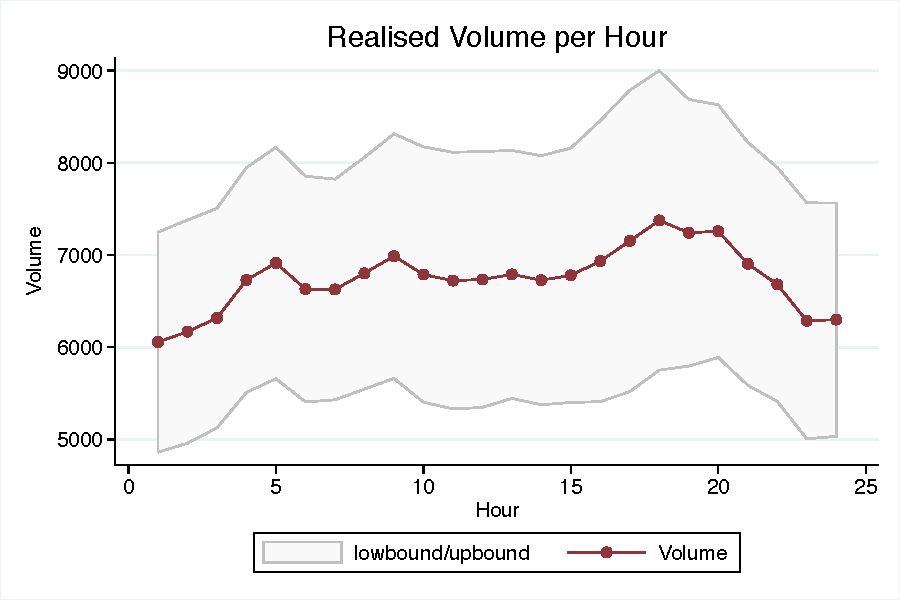
\includegraphics[height=50mm]{figch2/h1a.pdf} 
\hspace{0.05cm}
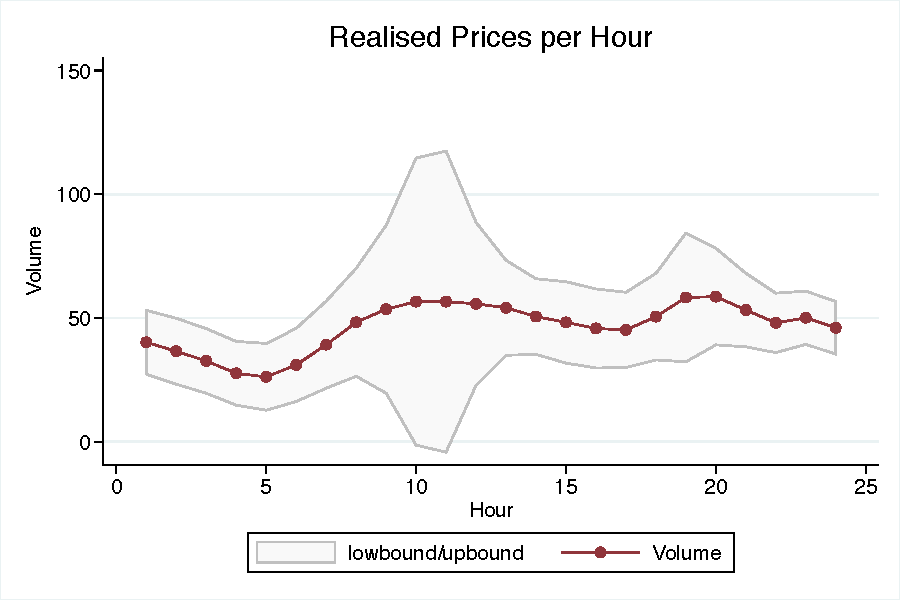
\includegraphics[height=50mm]{figch2/h1b.pdf} 
} 
\end{center}
\caption{\small Plotted average realised Volume (left) and Price (right) per Hour with 95\% confidence intervals.}
\label{EquilVolPriperHour}
\end{figure}


\begin{figure}[H]
\begin{center}
\makebox[\textwidth][c]{
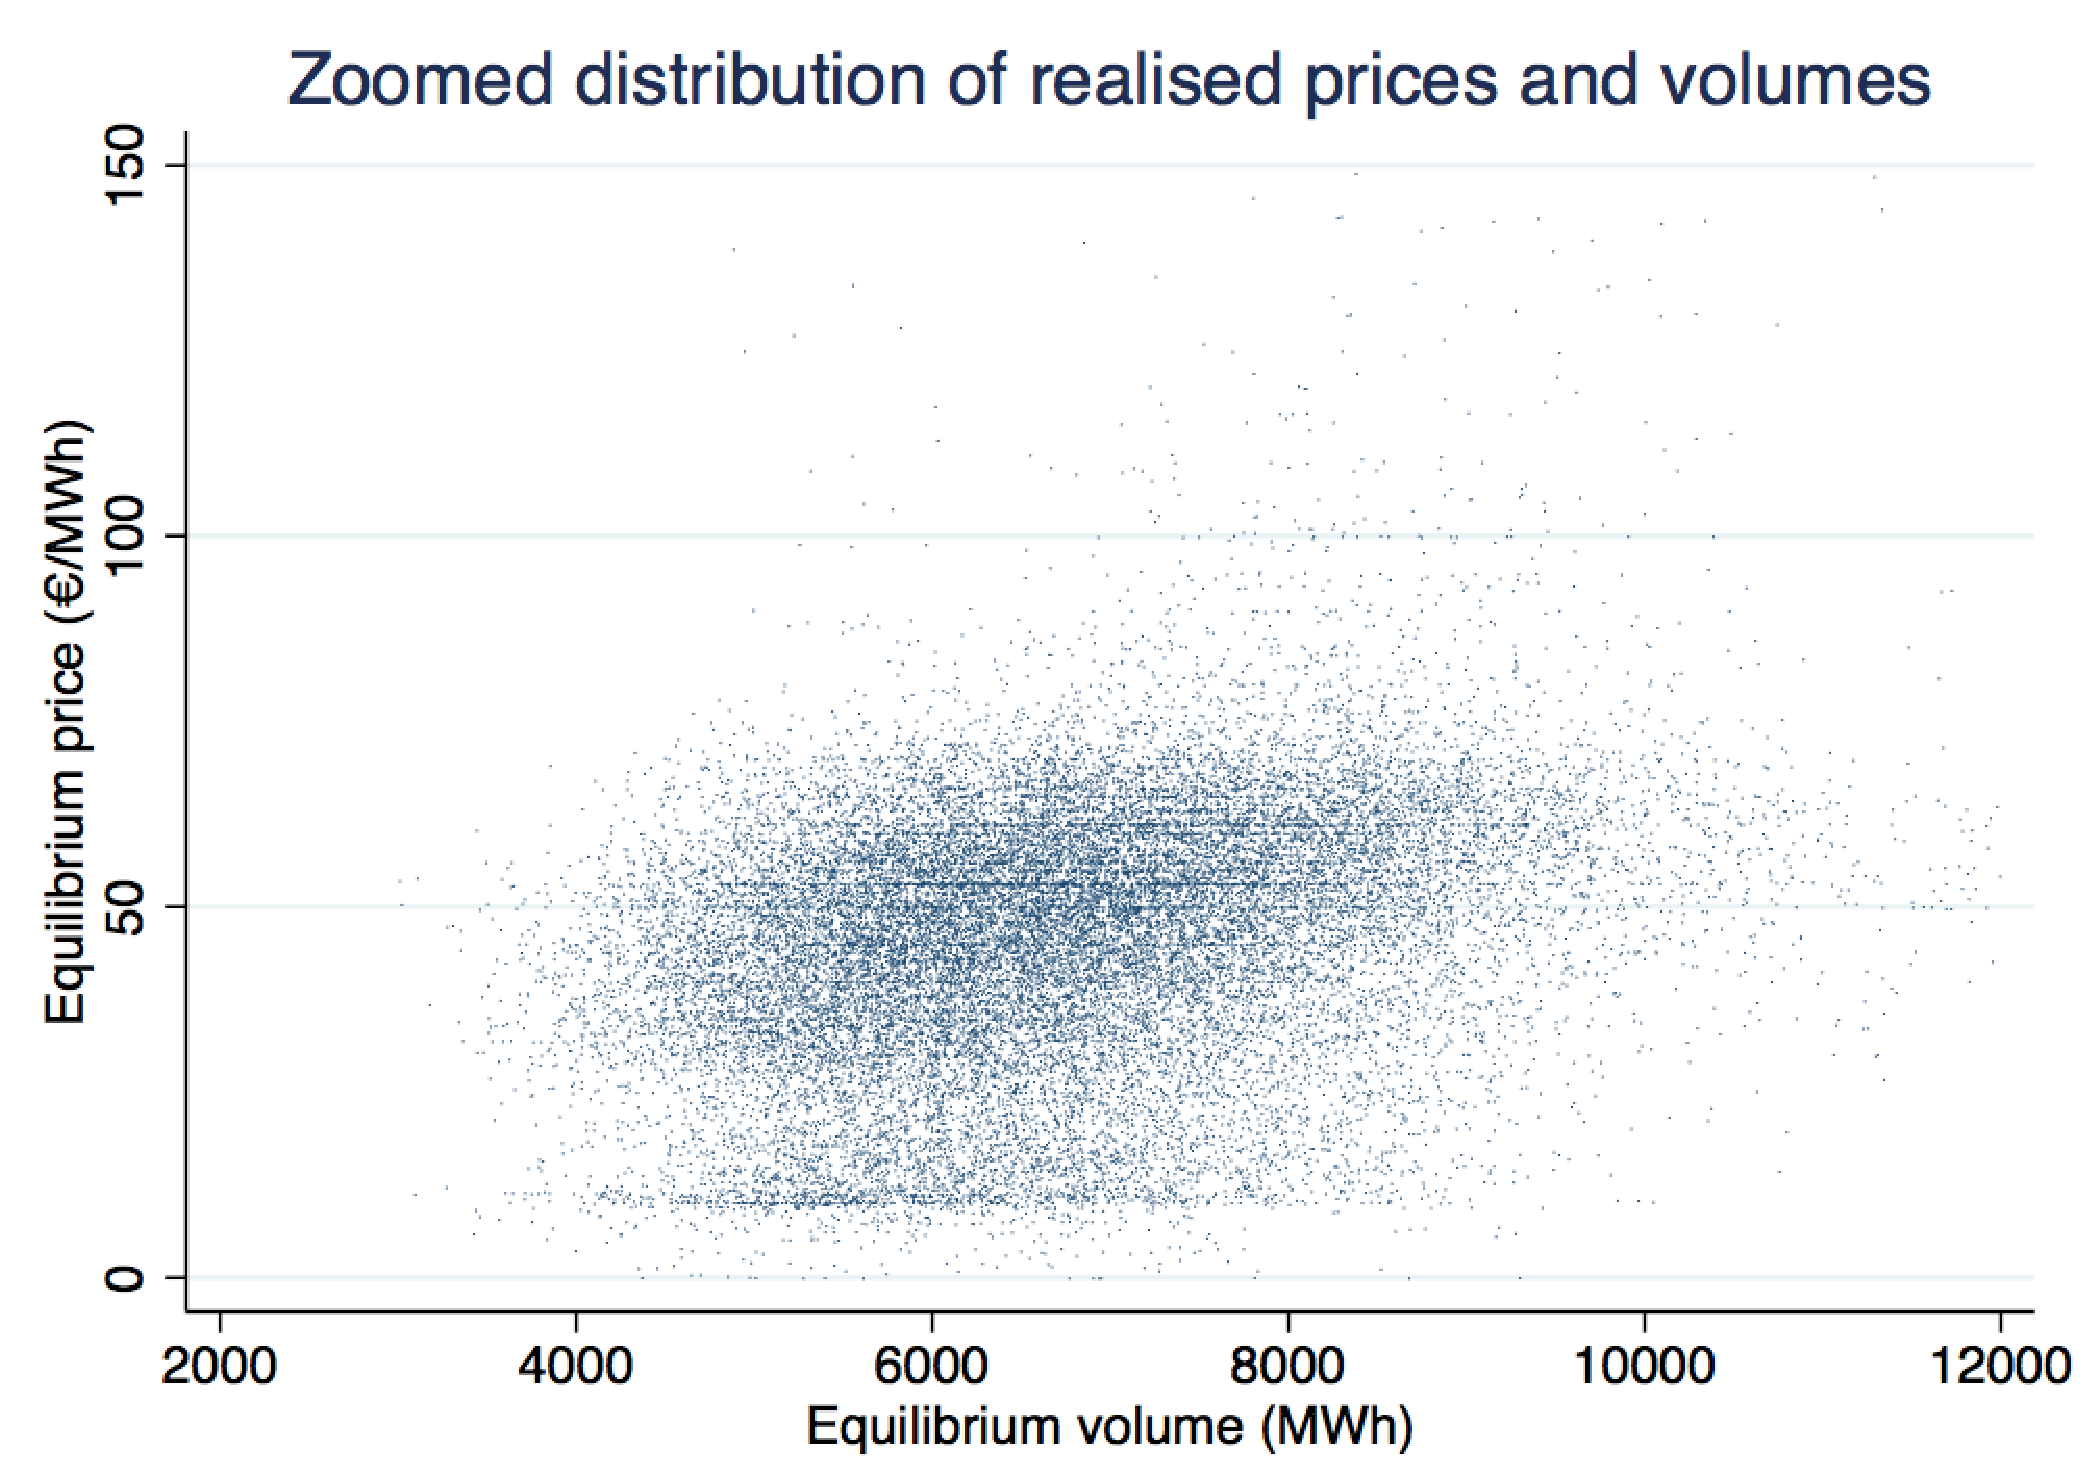
\includegraphics[trim=0cm 0cm 0cm 0cm, clip=true, height=45mm]{figch2/Shot16.pdf} 
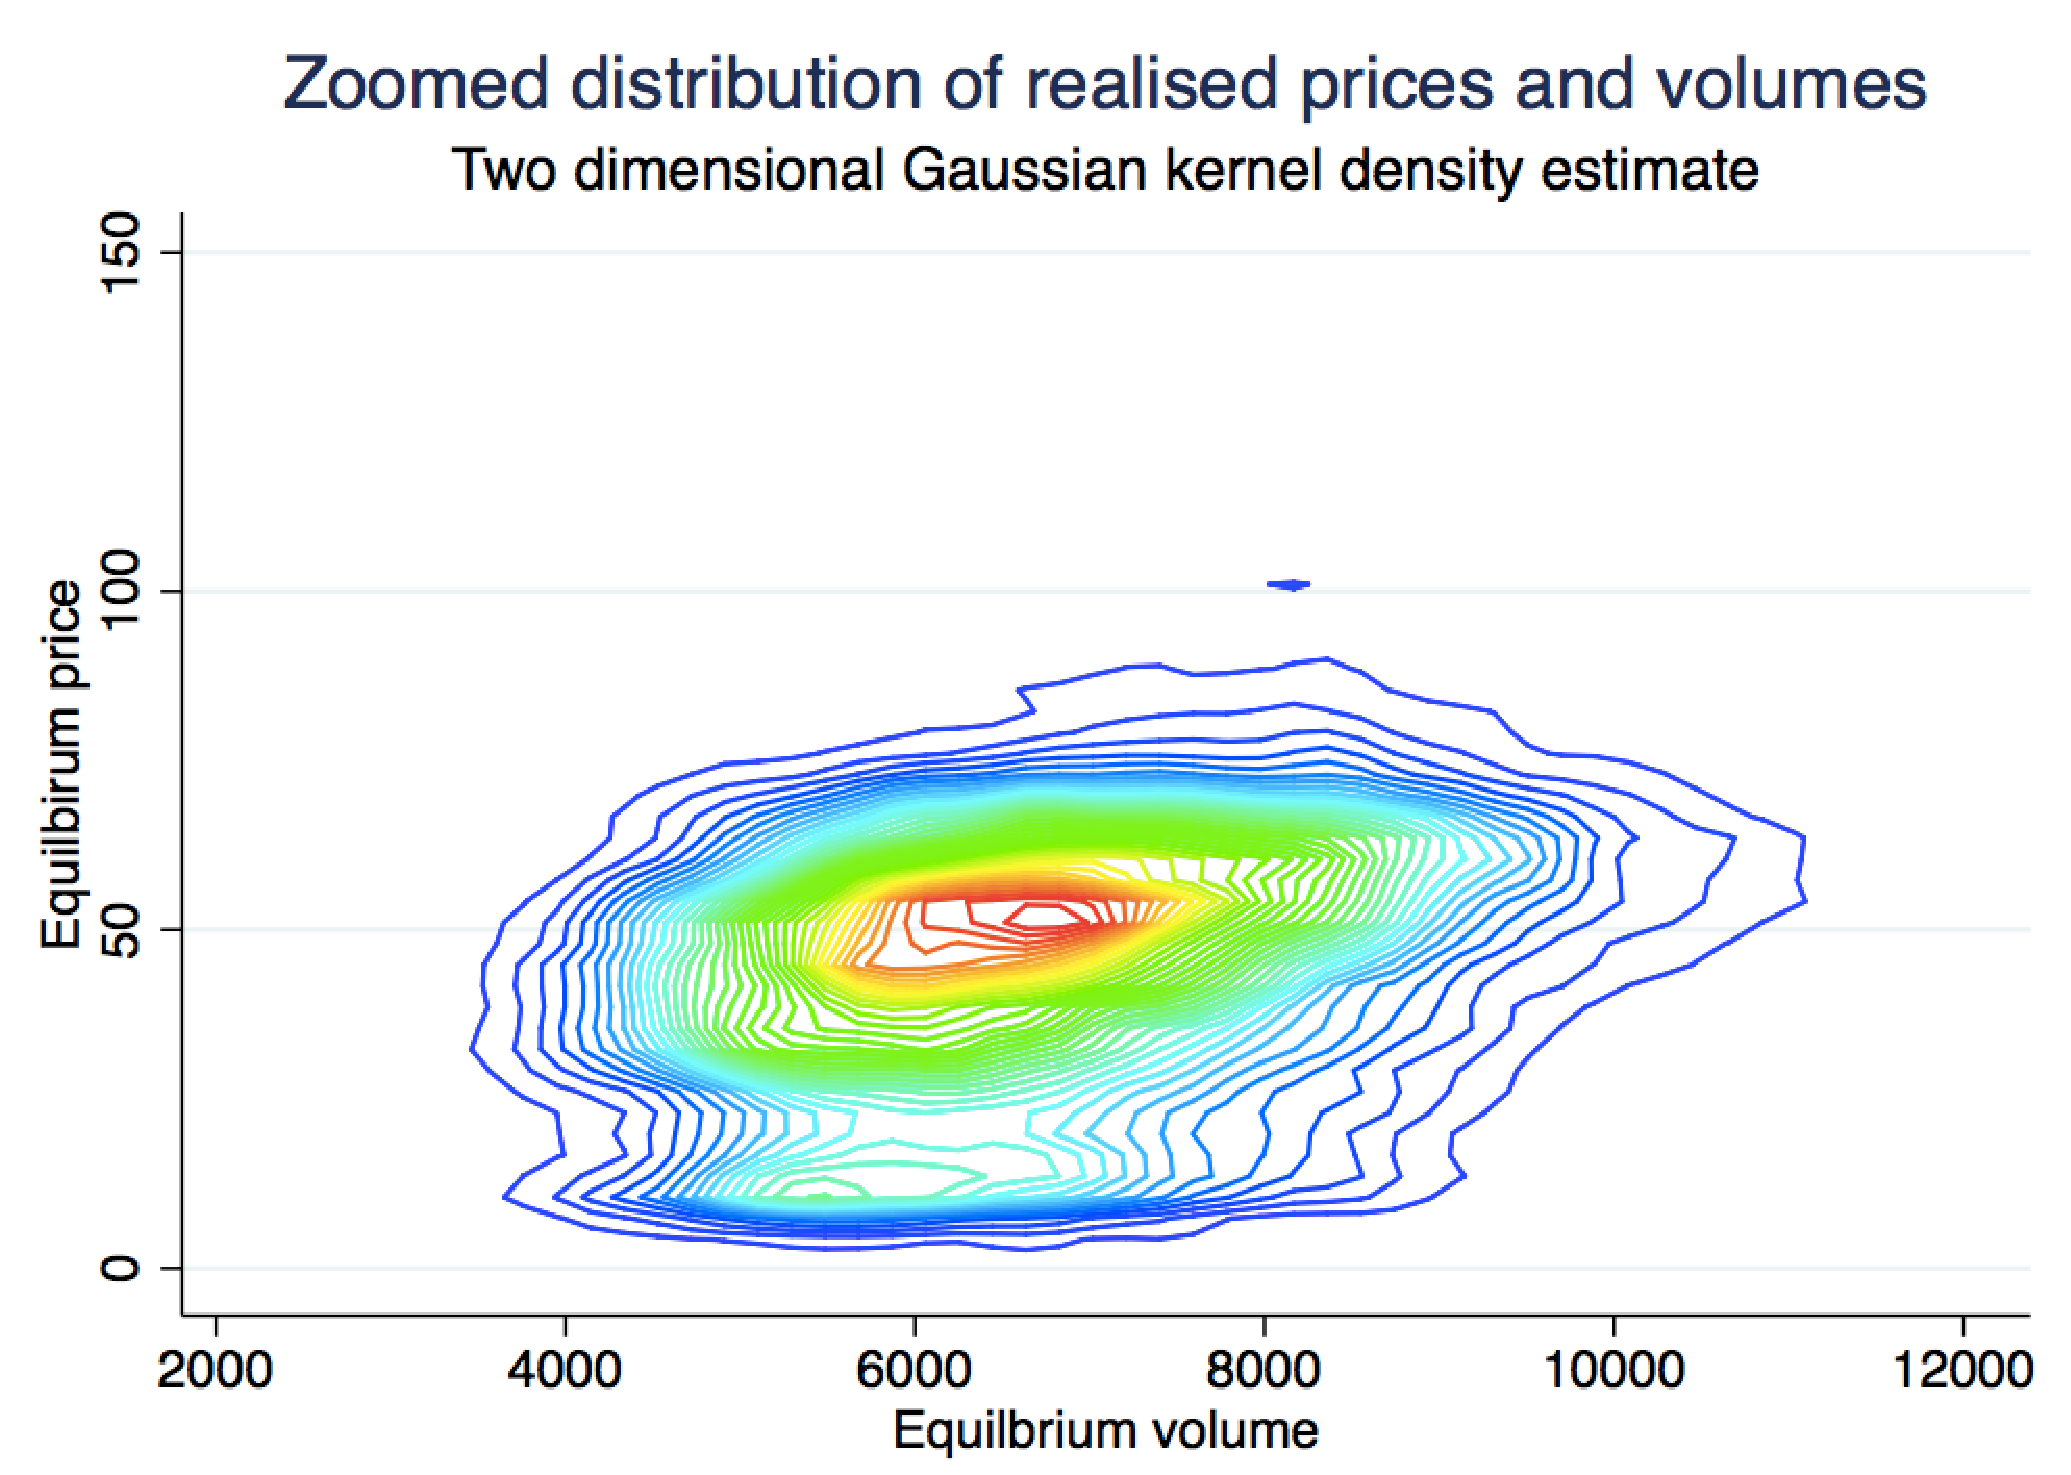
\includegraphics[trim=0cm 0cm 0cm 0cm, clip=true, height=45mm]{figch2/Shot01.pdf}
} 
\caption{Distribution of observed market equilibria}
\label{g7f}
\end{center}
{ \small Note: The warmer the colours of the heat map, the higher the frequency of realised price-quantity schedules. The colour legend is omitted for brevity, density changes between contours are of the order of $10^{-4}$.} 
\end{figure}

\label{statdes1}

\subsubsection{On player bid functions}
\begin{figure}[H]
\begin{center}
\makebox[\textwidth][c]{
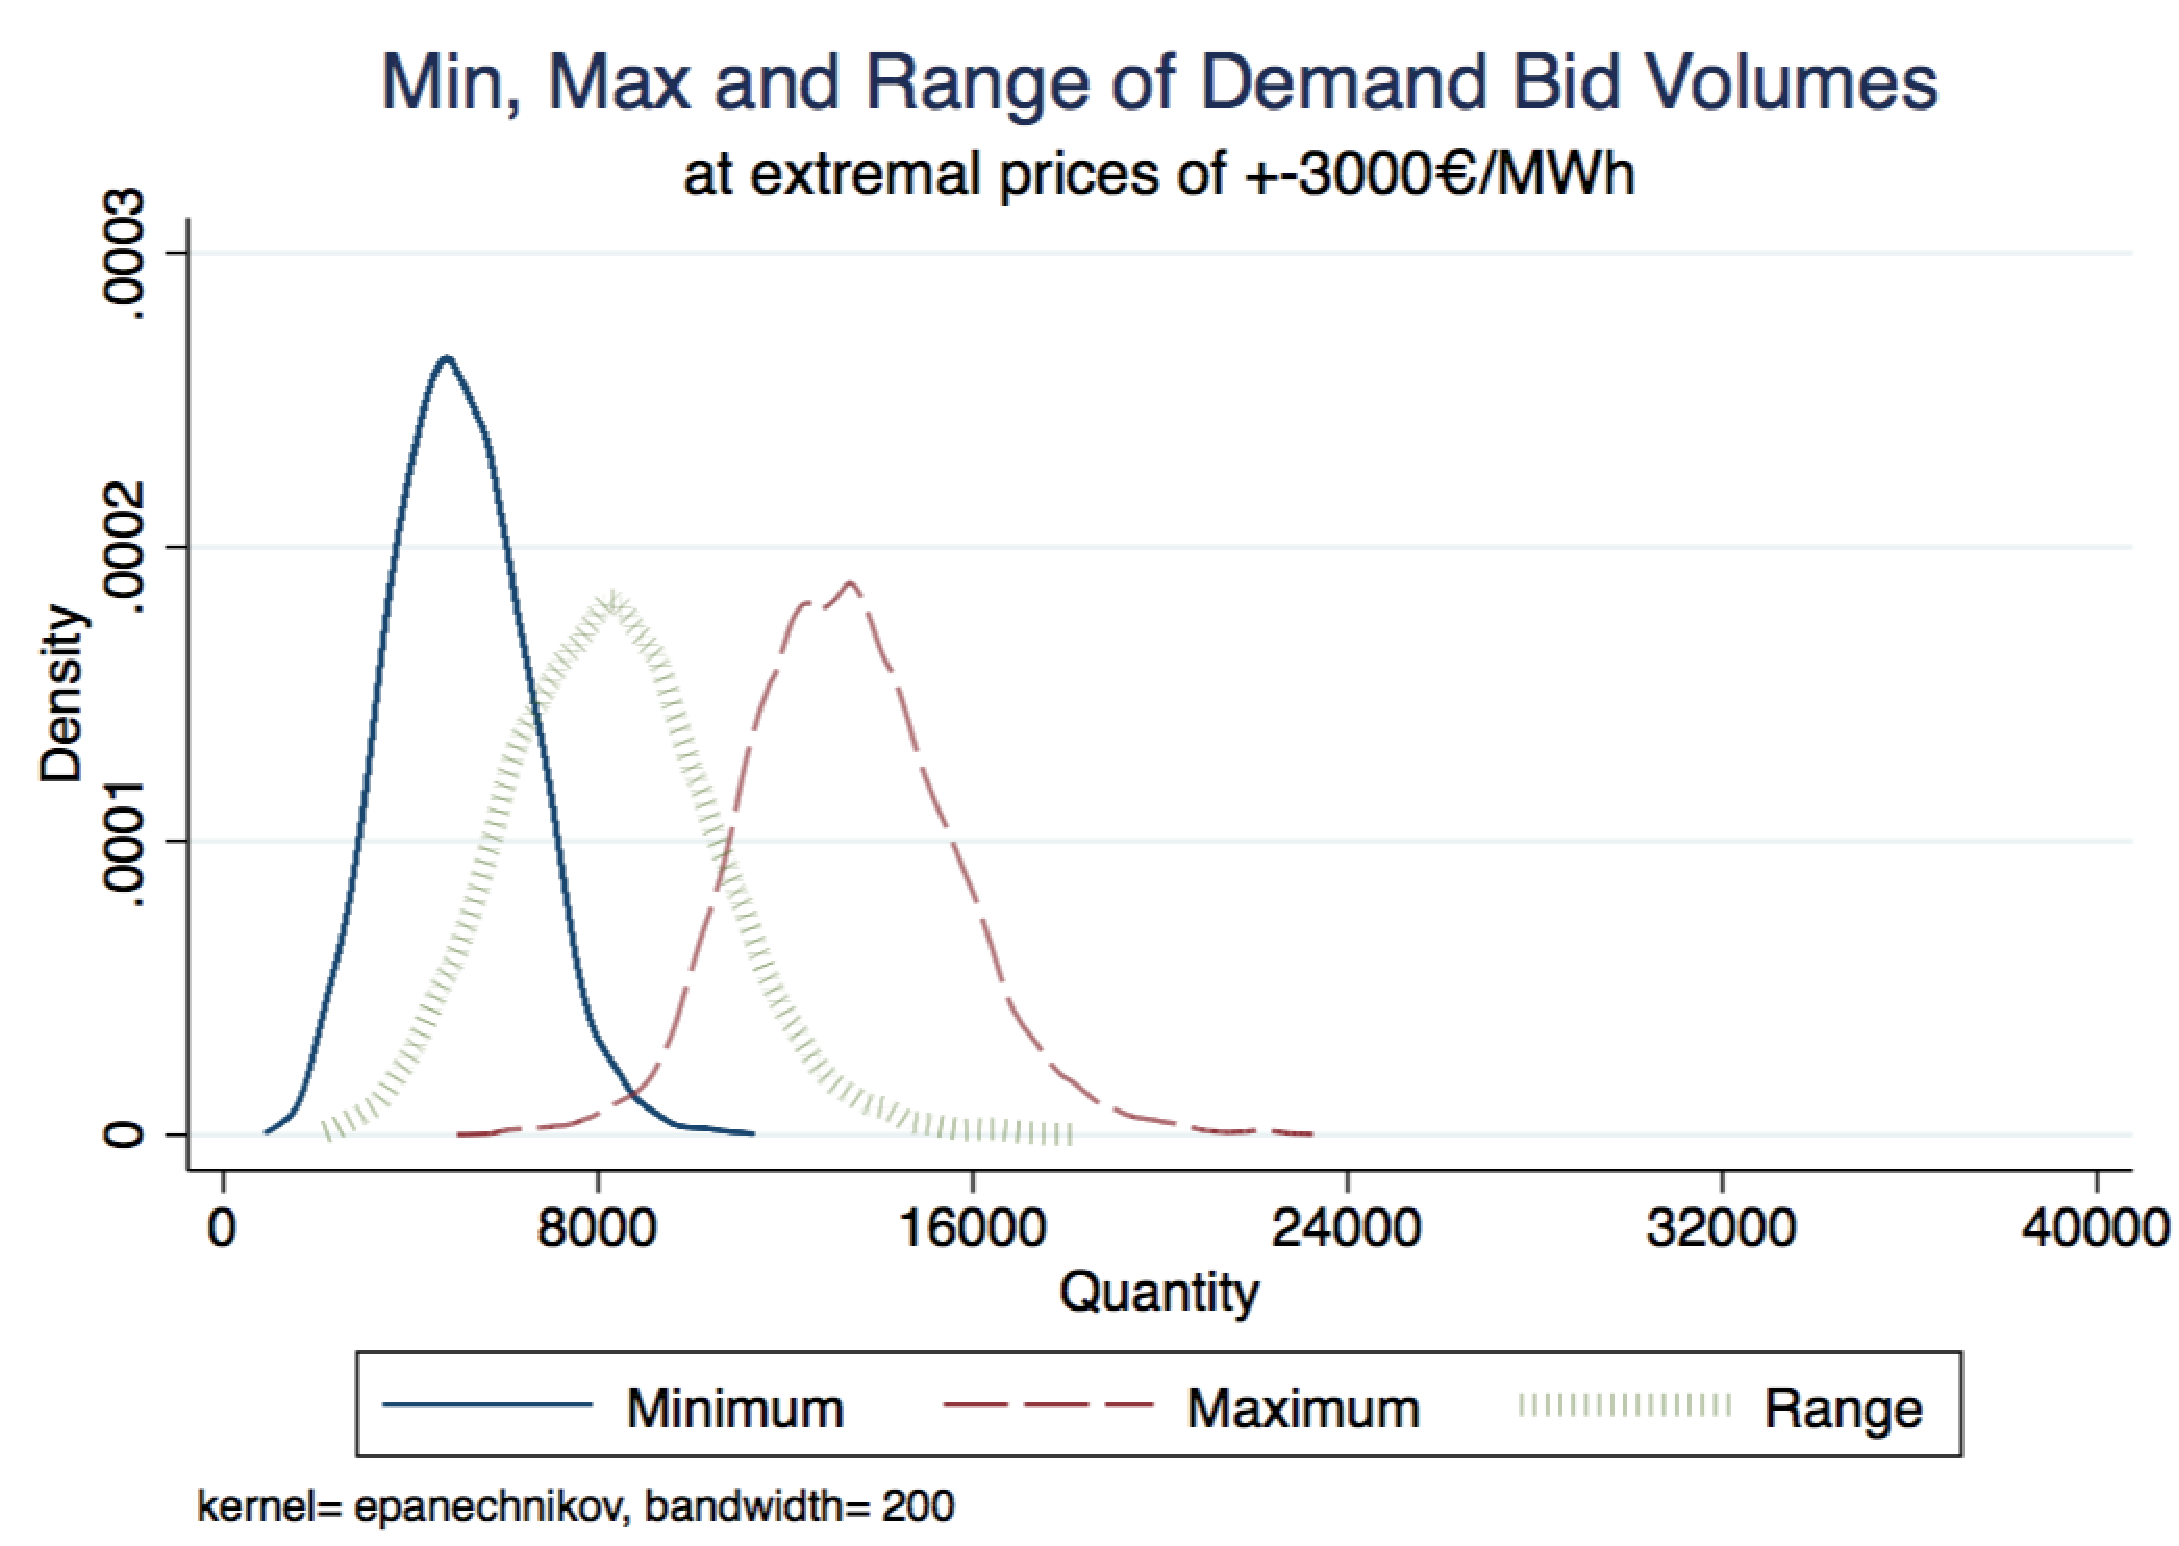
\includegraphics[height=45mm]{figch2/Shot20.pdf}  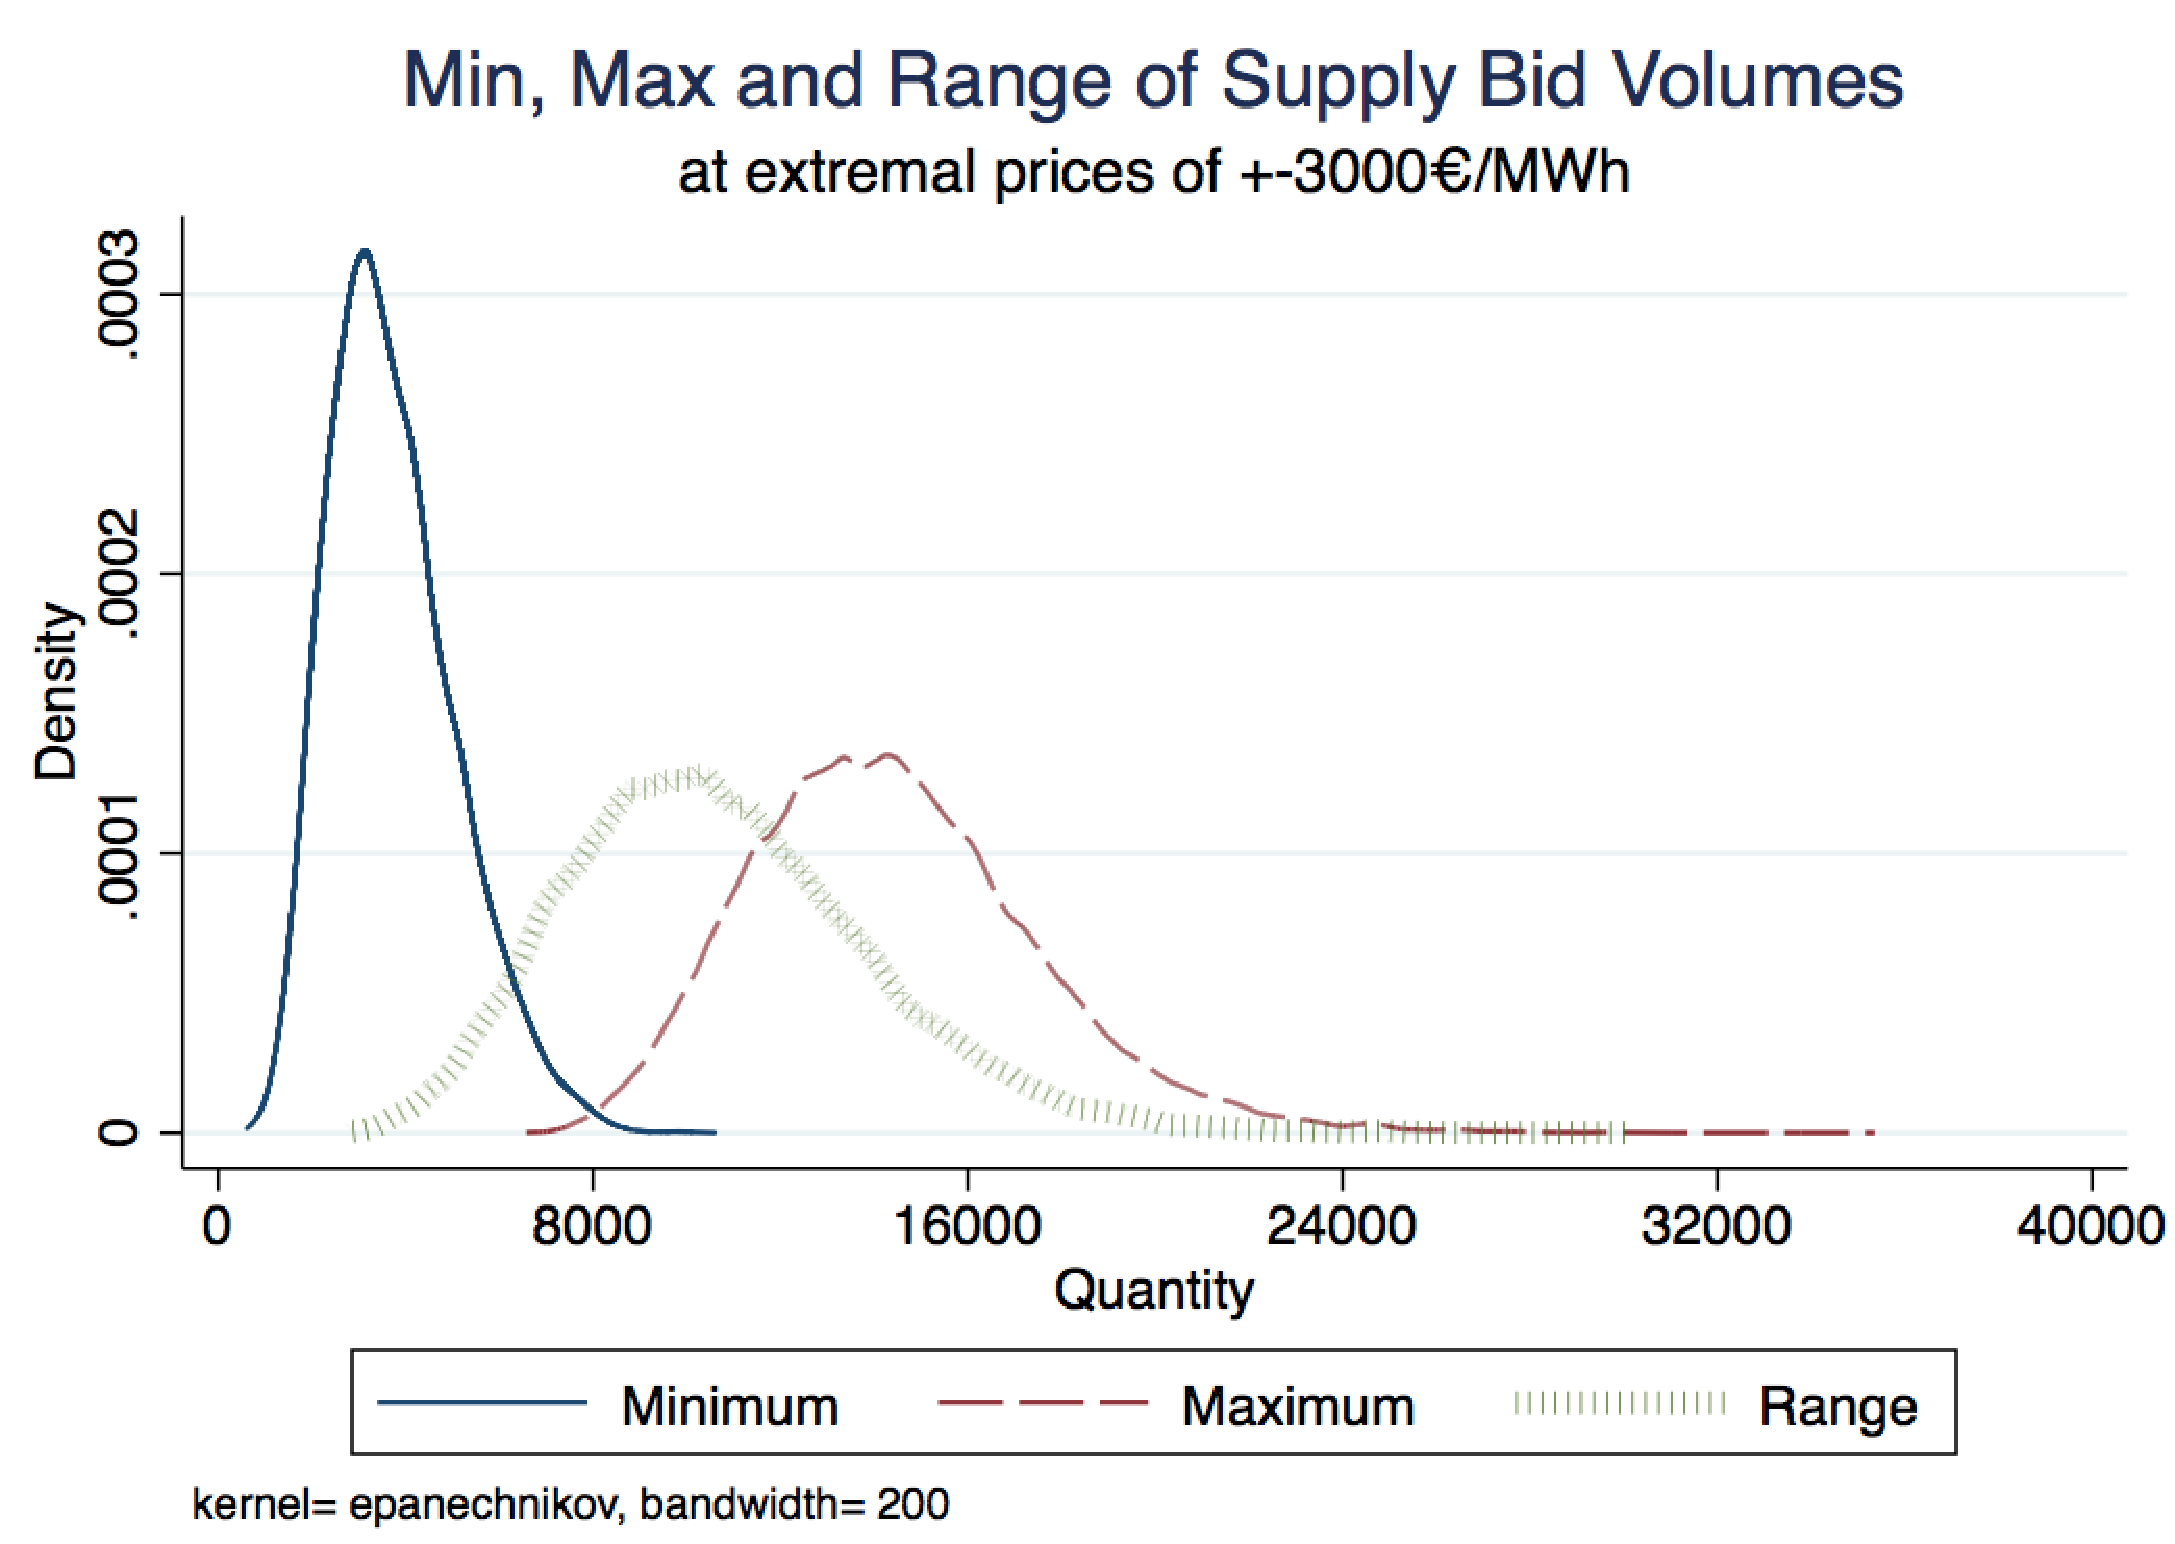
\includegraphics[height=45mm]{figch2/Shot21.pdf} 
}
\caption{Distribution of minimum and maximum production volumes (and corresponding range) bid in an hourly auction.}
\label{g9a}
\end{center}
\end{figure}
\begin{figure}[H]
\begin{center}
\makebox[\textwidth][c]{
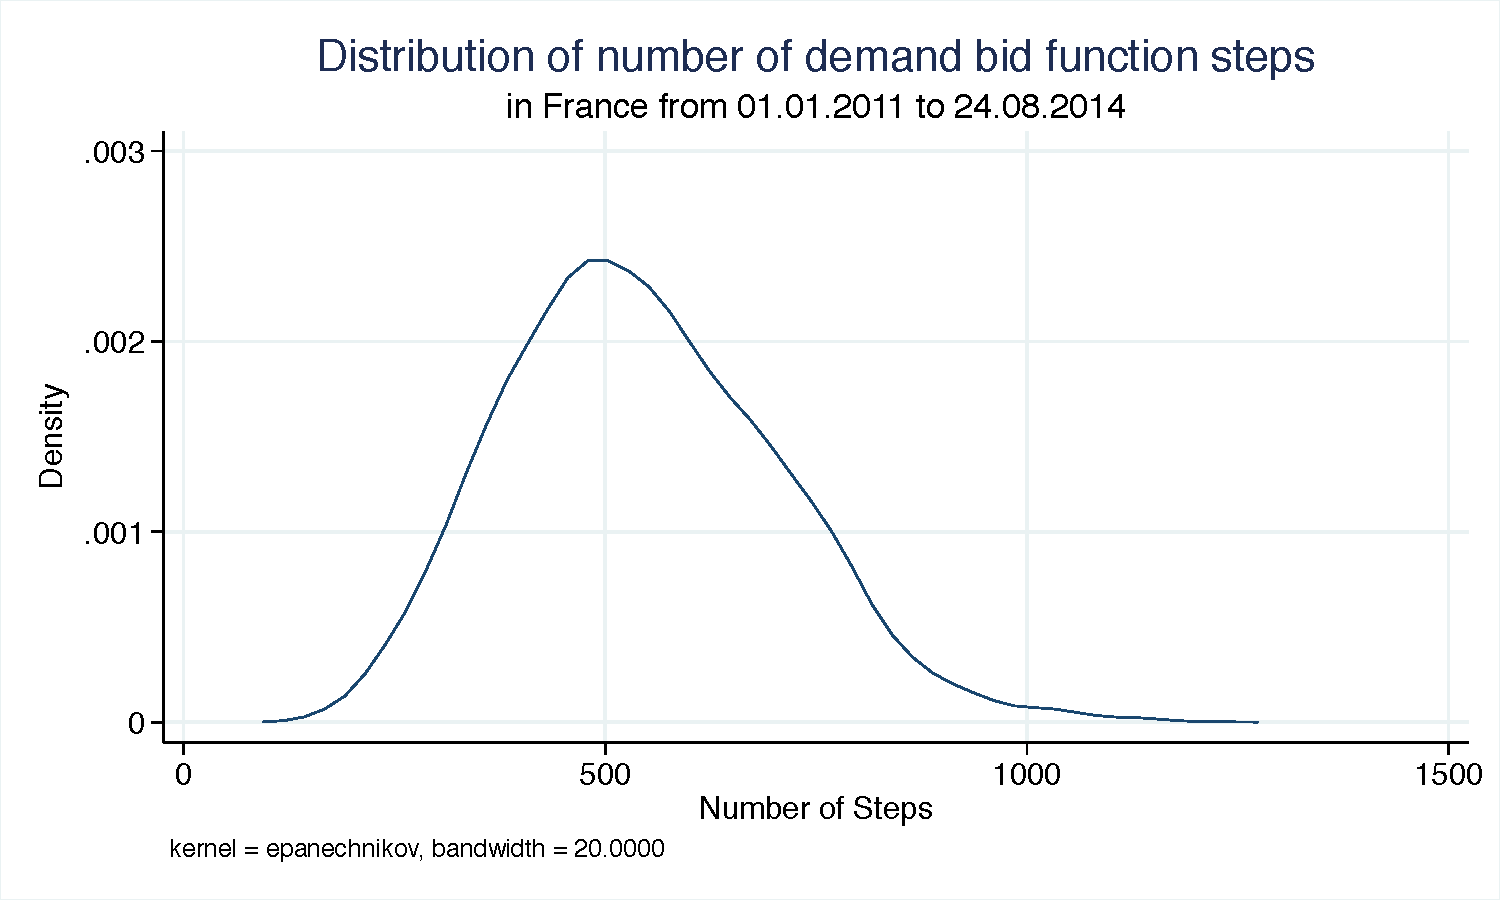
\includegraphics[trim=0cm 0cm 0cm 0cm, clip=true, height=45mm]{figch2/stepsD1.pdf} 
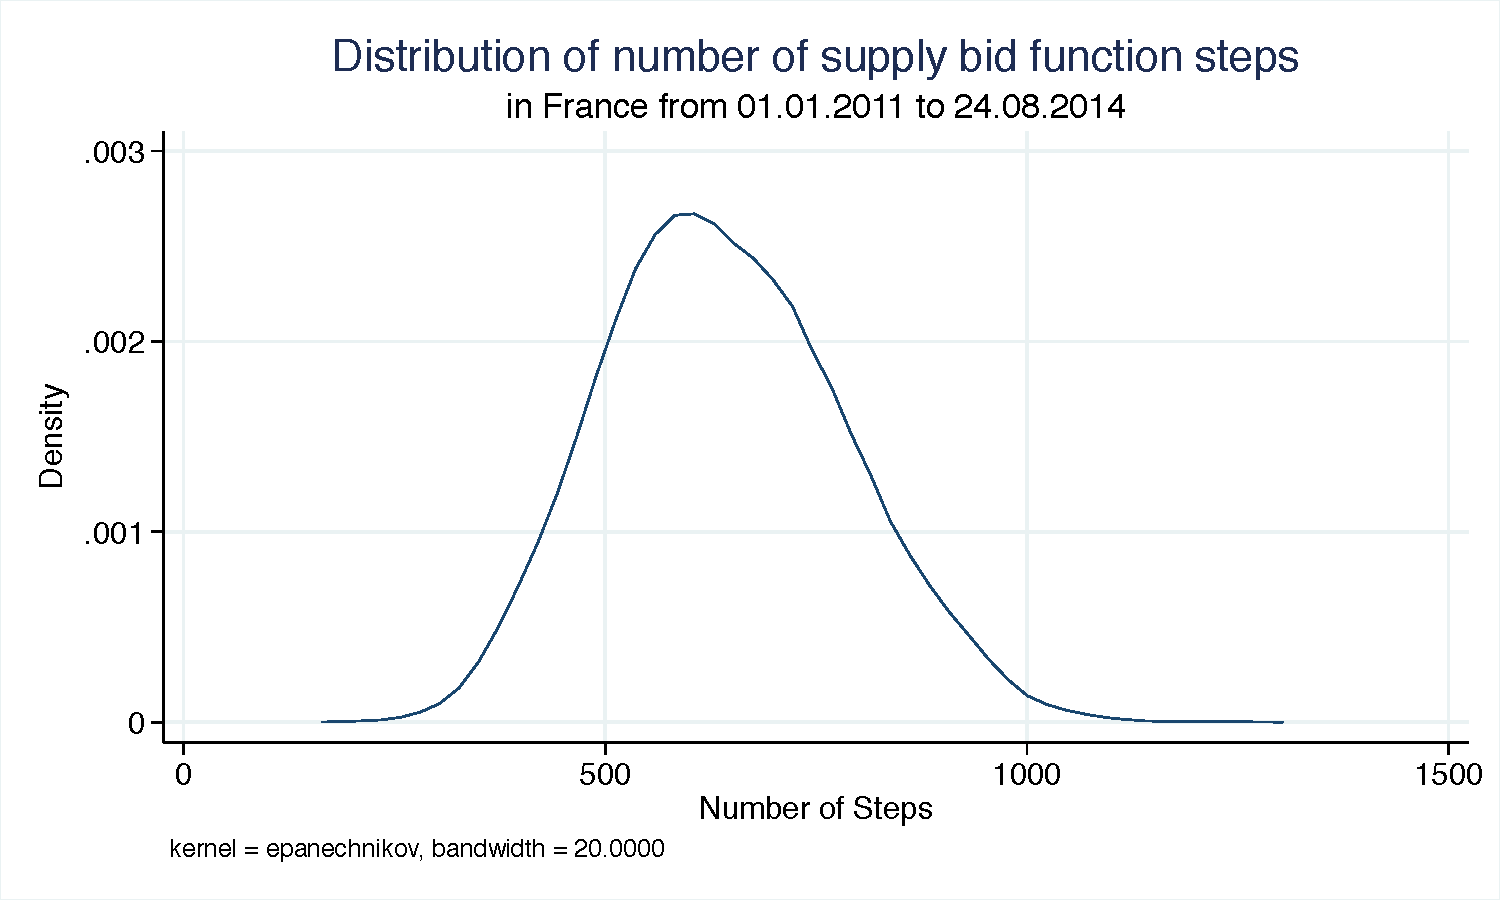
\includegraphics[trim=0cm 0cm 0cm 0cm, clip=true, height=45mm]{figch2/stepsS1.pdf} 
}
\caption{Distribution of number of bid function steps}
\label{steps}
\end{center}
\end{figure}


\subsubsection{On exogenous factors}
\label{statdesEXO}
\begin{figure}[H]
\begin{center}
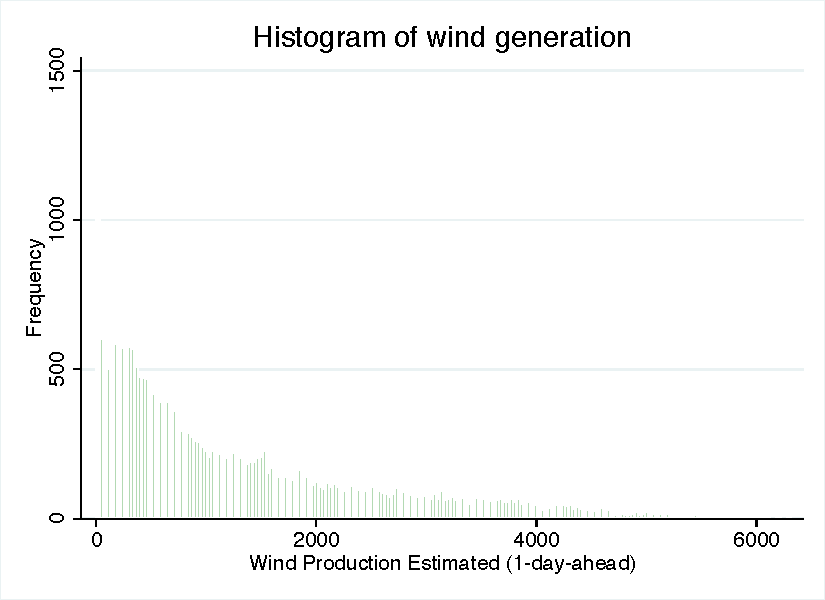
\includegraphics[trim=0cm 0cm 0cm 0cm, clip=true, height=45mm]{figch2/m1b.pdf} 
\hspace{0.05cm}
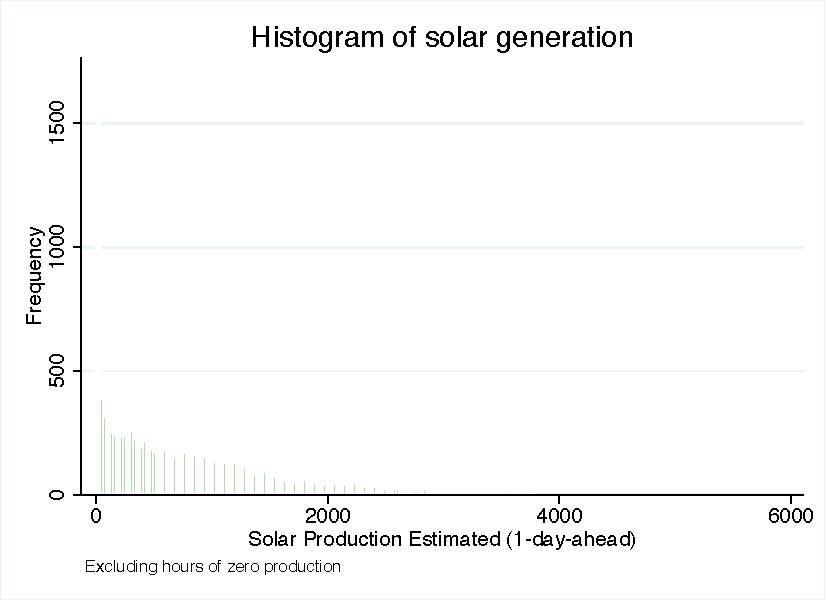
\includegraphics[trim=0cm 0cm 0cm 0cm, clip=true, height=45mm]{figch2/m2b.pdf} 
\caption{Histogram of predicted wind (left) and predicted solar (right) generation}
\label{m1b}
\end{center}
\end{figure}

\end{subappendices}















